% This template was originally by R. Jacob Vogelstein
% Updated on March 1, 2010 by Noah J. Cowan
% Updated by Brian D. Weitzner, April 29, 2014
% Edited March, 2016 by Karla Hernandez

\documentclass[12pt,oneside,final]{thesis}

\usepackage[english]{babel}
\usepackage{blindtext}

\newenvironment{bottompar}{\par\vspace*{\fill}}{\clearpage}

\usepackage{cite}
\usepackage{amsmath,amsfonts}
\DeclareMathOperator*{\argmax}{arg\,max}
\DeclareMathOperator*{\argmin}{arg\,min}

\usepackage{amsthm}
\newtheorem{theorem}{Theorem}
\newtheorem{corollary}{Corollary}
\newtheorem{lemma}{Lemma}
\newtheorem{proposition}{Proposition}
\theoremstyle{definition}
\newtheorem{definition}{Definition}
\theoremstyle{remark}
\newtheorem*{remark}{Remark}
\theoremstyle{remark}
\newtheorem*{example}{Example}

\usepackage{etoolbox}
\usepackage{framed}
\newcommand\enclosebox[2]{%
  \BeforeBeginEnvironment{#1}{\begin{#2}}%
  \AfterEndEnvironment{#1}{\end{#2}}%
}
\enclosebox{definition}{leftbar} % comment to remove left bar on definitions.
\enclosebox{remark}{leftbar} % comment to remove left bar on remarks.


\usepackage{graphicx}
\graphicspath{{./figs/}}
\usepackage{fixltx2e}
\usepackage{array}
\usepackage{wrapfig} 
\usepackage{newcent}

\usepackage[linktocpage=true]{hyperref} % Makes page numbers in table of contents clickable.

\usepackage{upgreek} % Allows you to use 
\usepackage{bm}
\usepackage{hyperref}
\usepackage{setspace}
\usepackage{booktabs}
\usepackage{multirow}
\usepackage{longtable}
\usepackage[font=singlespacing, labelfont=bf]{caption}
%\usepackage{CV}
\usepackage{rotating}
\usepackage{lscape}

% only single line spacing in tables
%\BeforeBeginEnvironment{tabular}{\begin{singlespace}}
%\AfterEndEnvironment{tabular}{\end{singlespace}}
%\BeforeBeginEnvironment{longtable}{\begin{singlespace}}
%\AfterEndEnvironment{longtable}{\end{singlespace}}

\usepackage{enumitem}
\newlist{inlinelist}{enumerate*}{1}
\setlist*[inlinelist,1]{%
  label=(\arabic*),
}

\usepackage{fancyhdr}    % Use nice looking headers along with the required footer page numbers   

%Define the header/footer style
\pagestyle{fancy}
\fancyhf{}
\setlength{\headheight}{15pt}
\lhead{\leftmark}
\cfoot{\thepage}
\renewcommand{\headrulewidth}{0pt} % Remove line on page header by setting to 0pt
\fancypagestyle{plain}{% Redefine ``plain'' style for chapter boundaries
\fancyhf{} % clear all header and footer fields
\fancyfoot[C]{\thepage} % except the center
\renewcommand{\headrulewidth}{0pt}
\renewcommand{\footrulewidth}{0pt}}


\usepackage{amsthm}

%\tolerance=10000
\newcommand{\q}[1]{``#1''}


\usepackage{glossaries}
%\renewcommand\glossaryname{Glossary of Terms}
%\renewcommand\glossarytitle{}
\makeglossary % enable the glossary


\begin{document}

\title{A computational search for mutational drivers in cancer}
\author{Collin Tokheim}
\degreemonth{Month}
\degreeyear{2018} 
\dissertation
\doctorphilosophy
\copyrightnotice


% add your chapters, best way is to have separate TeX files for each chapter
%!TEX root = root.tex

%% FRONTMATTER
\begin{frontmatter}

% generate title
\maketitle

\begin{abstract}

\Blindtext[3]

\vfill
\noindent {\bf{Primary Reader and Advisor:}} Rachel Karchin \\
{\bf{Secondary Reader:}} Someone Else
\end{abstract}

\begin{acknowledgment}

\blindtext

\end{acknowledgment}

\begin{dedication}
 
To my family

\end{dedication}

% generate table of contents
\tableofcontents

% generate list of tables
\listoftables

% generate list of figures
\listoffigures

\end{frontmatter}

%!TEX root = root.tex

\chapter{Introduction}
\label{chap:intro}
\chaptermark{Optional running chapter heading}

\section{Spacing \& Type}
\label{sec:section}

This is a section. This is a citation without brackets \citen{A}. and this is one with brackets \cite{A}. These are multiple citations: [\citen{A, B, C}]. Here's a reference to a subsection: \ref{sec:subsection}. The body of the text and abstract must be double-spaced except for footnotes or long quotations. Fonts such as Times Roman, Bookman, New Century Schoolbook, Garamond, Palatine, and Courier are acceptable and commonly found on most computers. The same type must be used throughout the body of the text. The font size must be 10 point or larger and footnotes\footnote{This is a footnote.} must be two sizes smaller than the text\footnote{This is another footnote.} but no smaller than eight points. Chapter, section, or other headings should be of a consistent font and size throughout the ETD, as should labels for illustrations, charts, and figures.  

\subsection{Creating a Subsection}
\label{sec:subsection}

\subsubsection{Creating a Subsubsection}

\paragraph{This is a heading level below subsubsection}

And this is a quote: 
%
\begin{quote}
\blindtext
\end{quote}

This is a table:
% currsize is not set in the long table environment, so we need to set it before we set it up.
\makeatletter
\let\@currsize\normalsize
\makeatother

% tabular environments are set to be single-spaced in the  thesis class,  but long tables do not use tabular
% to get around this, set the spacing to single spacing at the start of the long table environment, and set it back to double-spacing at the end of it
\ssp
\begin{longtable}{cc}
\caption[This is the title I want to appear in the List of Tables]{This is a caption.} \label{tab:pfams} \\
\hline
A & B \\
\hline
\endfirsthead
\multicolumn{2}{@{}l}{\textbf{Table \thetable} \ldots continued} \\
\hline
A & B \\
\hline
\endhead
a1 & b1 \\
a2 & b2 \\
a3 & b3 \\
a4 & b4 \\
\hline
\end{longtable}
\dsp

The package ``upgreek'' allows us to use non-italicized lower-case greek letters. See for yourself: $\upbeta$, $\bm\upbeta$, $\beta$, $\bm\beta$. Next is a numbered equation:
\begin{align}
\label{eq:name}
\|\bm{X}\|_{2,1}={\underbrace{\sum_{j=1}^nf_j(\bm{X})}_{\text{convex}}}=\sum_{j=1}^n\|\bm{X}_{.,j}\|_2
\end{align}
The reference to equation (\ref{eq:name}) is clickable. 

\section[Theorems, Corollaries, Lemmas, Proofs, Remarks, Definitions\\ and Examples]{Theorems, Corollaries, Lemmas,\\ Proofs, Remarks, Definitions,\\ and Examples}

\begin{theorem}
\label{thm:onlytheorem}
\blindtext
\end{theorem}

\begin{proof}
I'm a (very short) proof.
\end{proof}

\begin{lemma}
I'm a lemma.
\end{lemma}

\begin{corollary}
I include a reference to Thm. \ref{thm:onlytheorem}.
\end{corollary}

\begin{proposition}
I'm a proposition.
\end{proposition}

\begin{remark}
I'm a remark. 
\end{remark}

\begin{definition}
I'm a definition. I'm a definition. I'm a definition. I'm a definition. I'm a definition. I'm a definition. I'm a definition. I'm a definition. I'm a definition. I'm a definition. I'm a definition. 
\end{definition}

\begin{example}
I'm an example.
\end{example}


\section[Optional table of contents heading]{Section with\\ linebreaks in\\the
name}


\Blindtext[2]





%!TEX root = root.tex

\chapter{Statistically modeling the accumulation of somatic mutations in cancer}
\label{chap:ch2}
\chaptermark{Statistically modeling mutations}

Somatic mutations accumulate randomly in all cells of the body, starting from the beginning of embryogenesis through the entire lifetime of a person \cite{RN63}. Somatic mutations arise because of both endogenous and exogenous sources, or from a mutator phenotype acquired in a cancer cell. Endogenous sources include intrinsic DNA replication mistakes, damage caused by free radicals from metabolism, and spontaneous deamination of nucleotides \cite{RN64}. In contrast, exogenous sources originate from the environment and include ultraviolet radiation \cite{RN64} and various mutagenic chemicals like aristolochic acid \cite{RN65}.  Also, defective DNA damage repair in a cancer cell may lead to a mutator phenotype where a substantial number of unrepaired mutations become fixed, such as defective mismatch repair genes leading to microsatellite instability \cite{RN68}. Each mutational source leaves a mark on the cancer genome that reflects the mutational signatures during the lifetime of the cell's progeny leading to cancer \cite{RN64}.

\section{Variability in the background accumulation of mutations}

To investigate the potential for using elevated mutation rate per base as a means to detect cancer drivers, I sought to examine the background variability of mutation rate in human cancers. The median background mutation rate per base for each cancer type in my pan-cancer data set \cite{RN70} varied by over two orders of magnitude (\autoref{fig:mut_rate_variability}), with individual samples varying over an even larger range, which is consistent with prior observations \cite{RN13, RN51}. Because only a small fraction of the total somatic mutations in any common solid tumor affects driver genes, the remaining mutations can be considered passengers. The total number of mutations (drivers plus passengers) per base is therefore only slightly larger than the number of passenger mutations per base, and, for simplicity, I refer to this number as the background mutation rate. Mutation rates are also known to vary across the genome \cite{RN13} and are influenced by nucleotide context, gene expression, chromatin state, transcription factor occupancy, replication timing, DNA strand, and perhaps by a variety of factors that have yet to be discovered \cite{RN72, RN73, RN51, RN74}. For example, melanoma mutations in The Cancer Genom Atlas (TCGA) are predominately C to T transition mutations, which is not seen in other cancer types (\autoref{fig:mutation_context}).

\begin{figure}
  \centering
  \makeatletter
  \let\@currsize\normalsize
  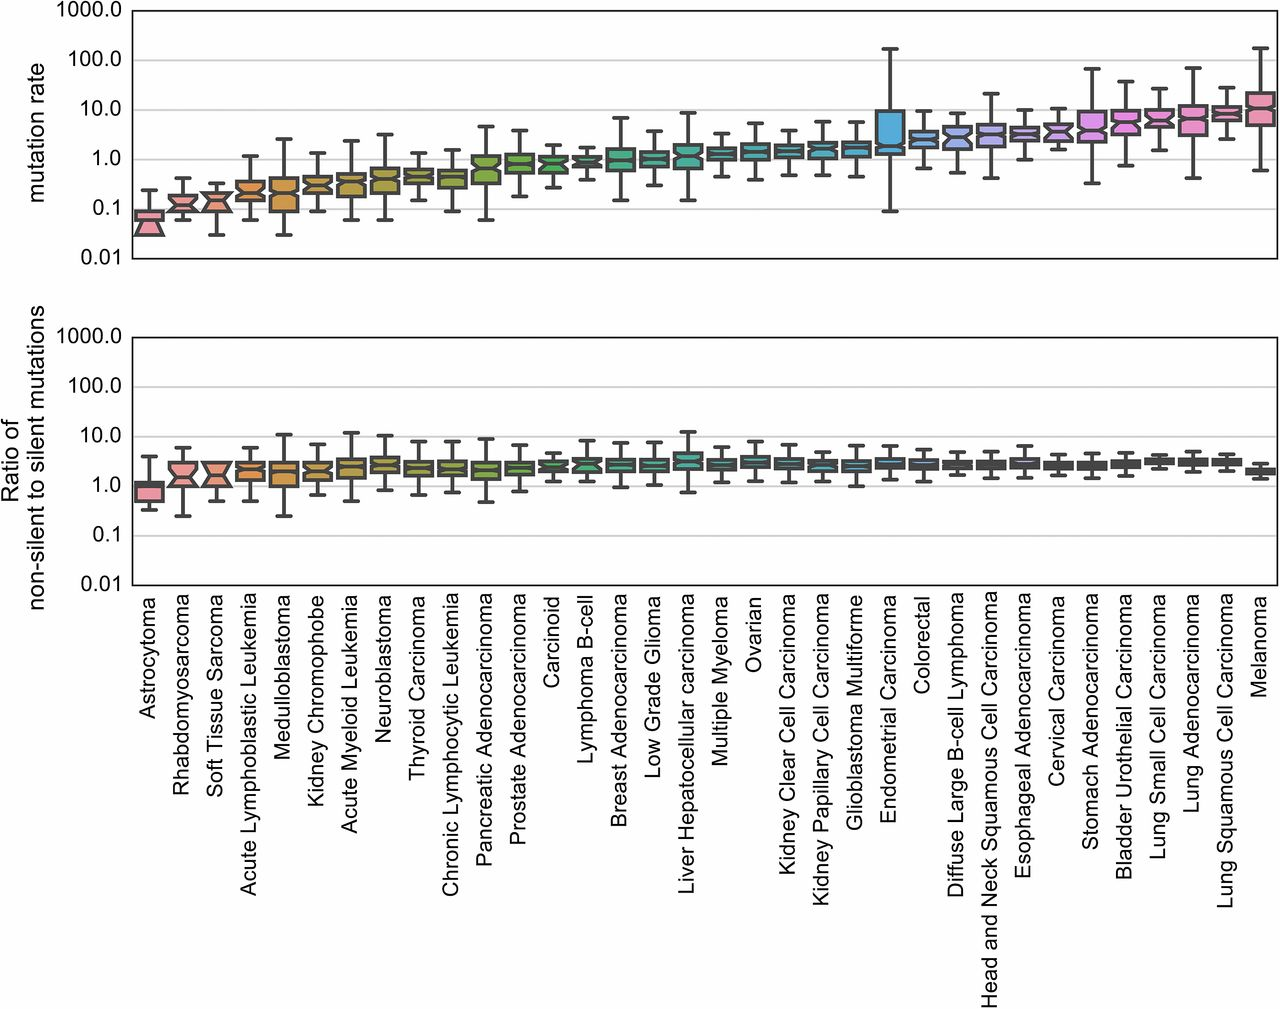
\includegraphics[width=0.9\linewidth]{figures/chapter2/mut_rate_and_ratiometric.jpg}
  \caption[Background mutation rate variability]{Background mutation rate is more variable than the ratio of nonsilent to silent mutations across 34 cancer types in data from \cite{RN14, RN71}. Boxplots are plotted on a log10 scale. The top boxplot shows the mutation rate in coding sequence for the samples in our pancancer dataset. The bottom boxplot shows the ratio of nonsilent to silent mutations in coding sequence for the same samples. A pseudocount for a silent mutation was added for each sample to avoid dividing by zero. Notches indicate bootstrap 95\% confidence interval (1,000 iterations) for the median. Outliers, defined as 1.5*IQR away from the first and third quartile, are not shown.}
  \label{fig:mut_rate_variability}
\end{figure}

\begin{figure}
  \centering
  \makeatletter
  \let\@currsize\normalsize
  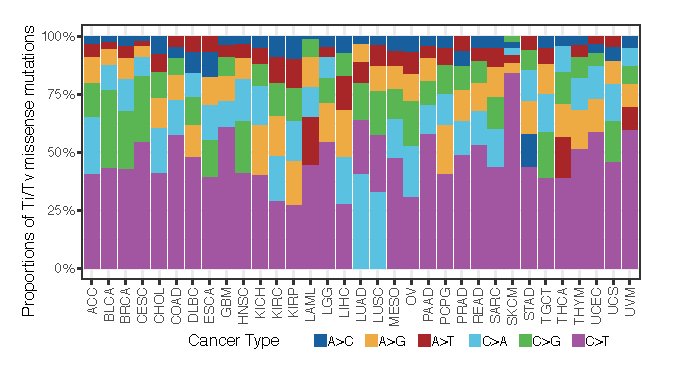
\includegraphics[width=0.9\linewidth]{figures/chapter2/mutation_context.pdf}
  \caption[Transition and transversion proportions in cancer]{Transition and transversion proportions are shown for 6 nucleotide changes from 33 cancer types available from the The Cancer Genome Atlas (https://synapse.org/MC3). The stacked proportion bar chart is sorted by increasing transition/transversion fraction.}
  \label{fig:mutation_context}
\end{figure}

However, mutation rate is not the only statistic capable of associating cancer drivers. One alternative is to use ratiometric features that normalize for the total number of mutations within a gene. For example, the ratio of non-silent to silent mutations within a gene is relative to silent mutations. Fig 1 shows the variability of the median ratio of non-silent to silent mutations for cancer types in our pancancer set. Ratiometric features had significantly less variability among cancer types than background mutation rates. The considerably lower variability suggests less factors would need to be modeled when developing a statistical model of somatic mutations.

\section{Expected consequence of variable background mutation rate}

\subsection{Increased mutational heterogeneity results in reduced statistical power or increased false positives}

I analyzed the possible impact of unexplained variability in background mutation rate on expected false-positive driver gene predictions. First, I applied a binomial model previously used for driver gene detection power analysis \cite{RN14}. The model assumes a gene-specific background mutation rate μ, which is set to a relatively high value, corresponding to genes in the 90th percentile of genes for mutation rate. I used the binomial to set a critical value for driver gene prediction, that is, the number of mutations required for a gene to be considered significantly different from the background. Next, I modeled the situation where the genes actually had mutation rates that varied around μ, using a beta-binomial model. I estimated the false positives expected under the binomial, after a highly conservative multiple-testing correction (Bonferroni), for levels of variability [beta-binomial coefficients of variation (CVs)], and for sample size ranging up to 8,000 (\autoref{fig:expected_fp}). Levels of variability defined by CVs (CV = 0.05, 0.1, and 0.2) were chosen to approximate low, medium, and high unexplained variation around the mean. As the number of samples increased, so did the number of expected false positives. At the low end of background mutation rates (0.5 mutations per megabase (MB)), the expected false positives remained low, even when 8,000 samples were evaluated, regardless of the level of variability. At an intermediate background mutation rate of 3.0 mutations per MB and with high unexplained variability, ∼1,000 false positives were expected from 8,000 samples. At a high background mutation rate (10.0 mutations per MB), both medium and high unexplained variability produced many thousand expected false positives.

\begin{figure}
  \centering
  \makeatletter
  \let\@currsize\normalsize
  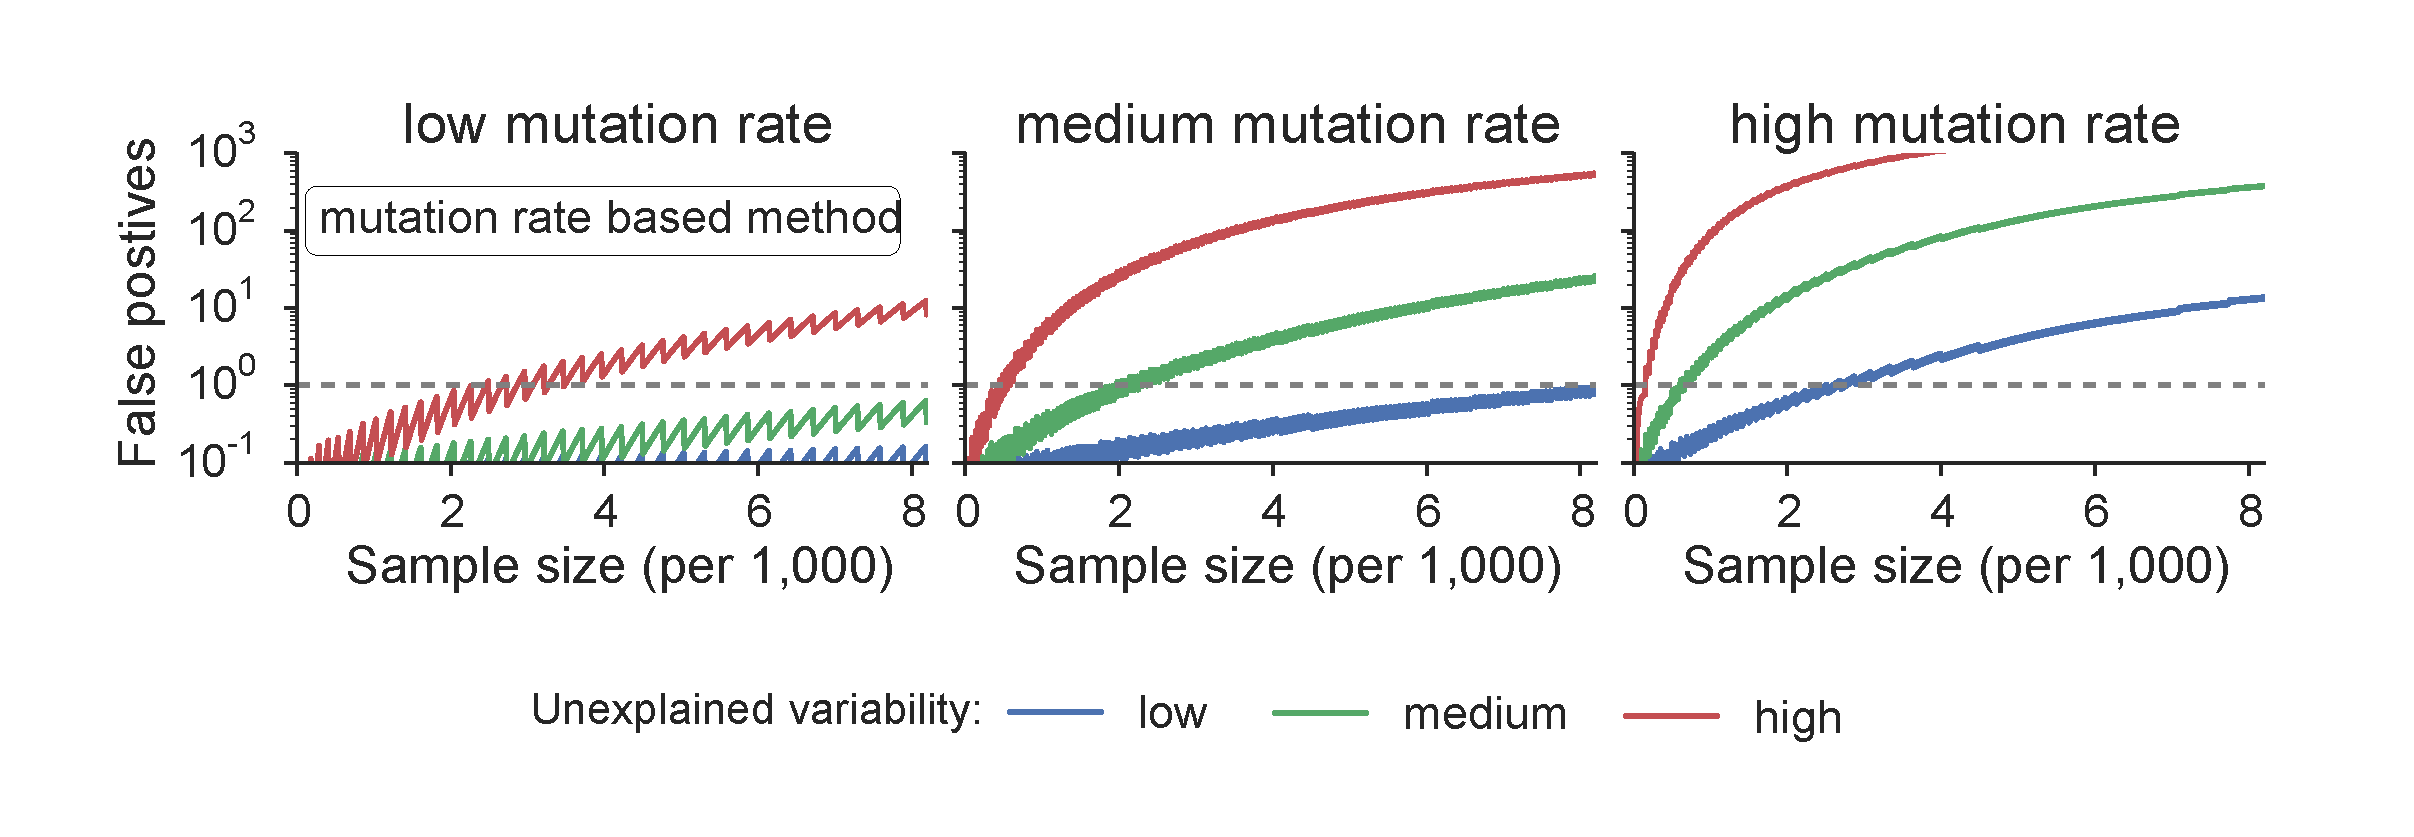
\includegraphics[width=0.9\linewidth]{figures/chapter2/expected_false_positives_mutation_rate.pdf}
  \caption[Expected false positives for driver gene detection]{Expected false positives for a mutation rate-based predictor that identifies genes with increased mutation rate over background.}
  \label{fig:expected_fp}
\end{figure}

I reasoned that unexplained variability might also have an impact on power calculations to estimate how many samples must be sequenced to find the majority of cancer driver genes. To this end, I repeated previous calculations performed with a binomial power model, in which the required sample size was estimated to be 600-5,000 per cancer type \cite{RN14}. The original model was parameterized to detect intermediate frequency driver genes, having 2-20\% mutation rates above background per sample, with background defined by genes in the 90th percentile of background mutation rates. First, I calculated the sample size required to detect 90\% of these drivers, given exome-wide backgrounds of 0.1-10 mutations per MB, and a conservative estimate of 2\% effect size (see statistical modeling of mutation rate). Next, I calculated the sample size required if the gene mutation rate varied around the original estimate, using a beta-binomial model with different CVs (CV = 0.05, 0.1, 0.2). The binomial power model was in accord with previous estimates. However, when unexplained variability was taken into account, the number of required samples increased sharply, particularly for higher background mutation rates (\autoref{fig:statistical_power}).

\begin{figure}
  \centering
  \makeatletter
  \let\@currsize\normalsize
  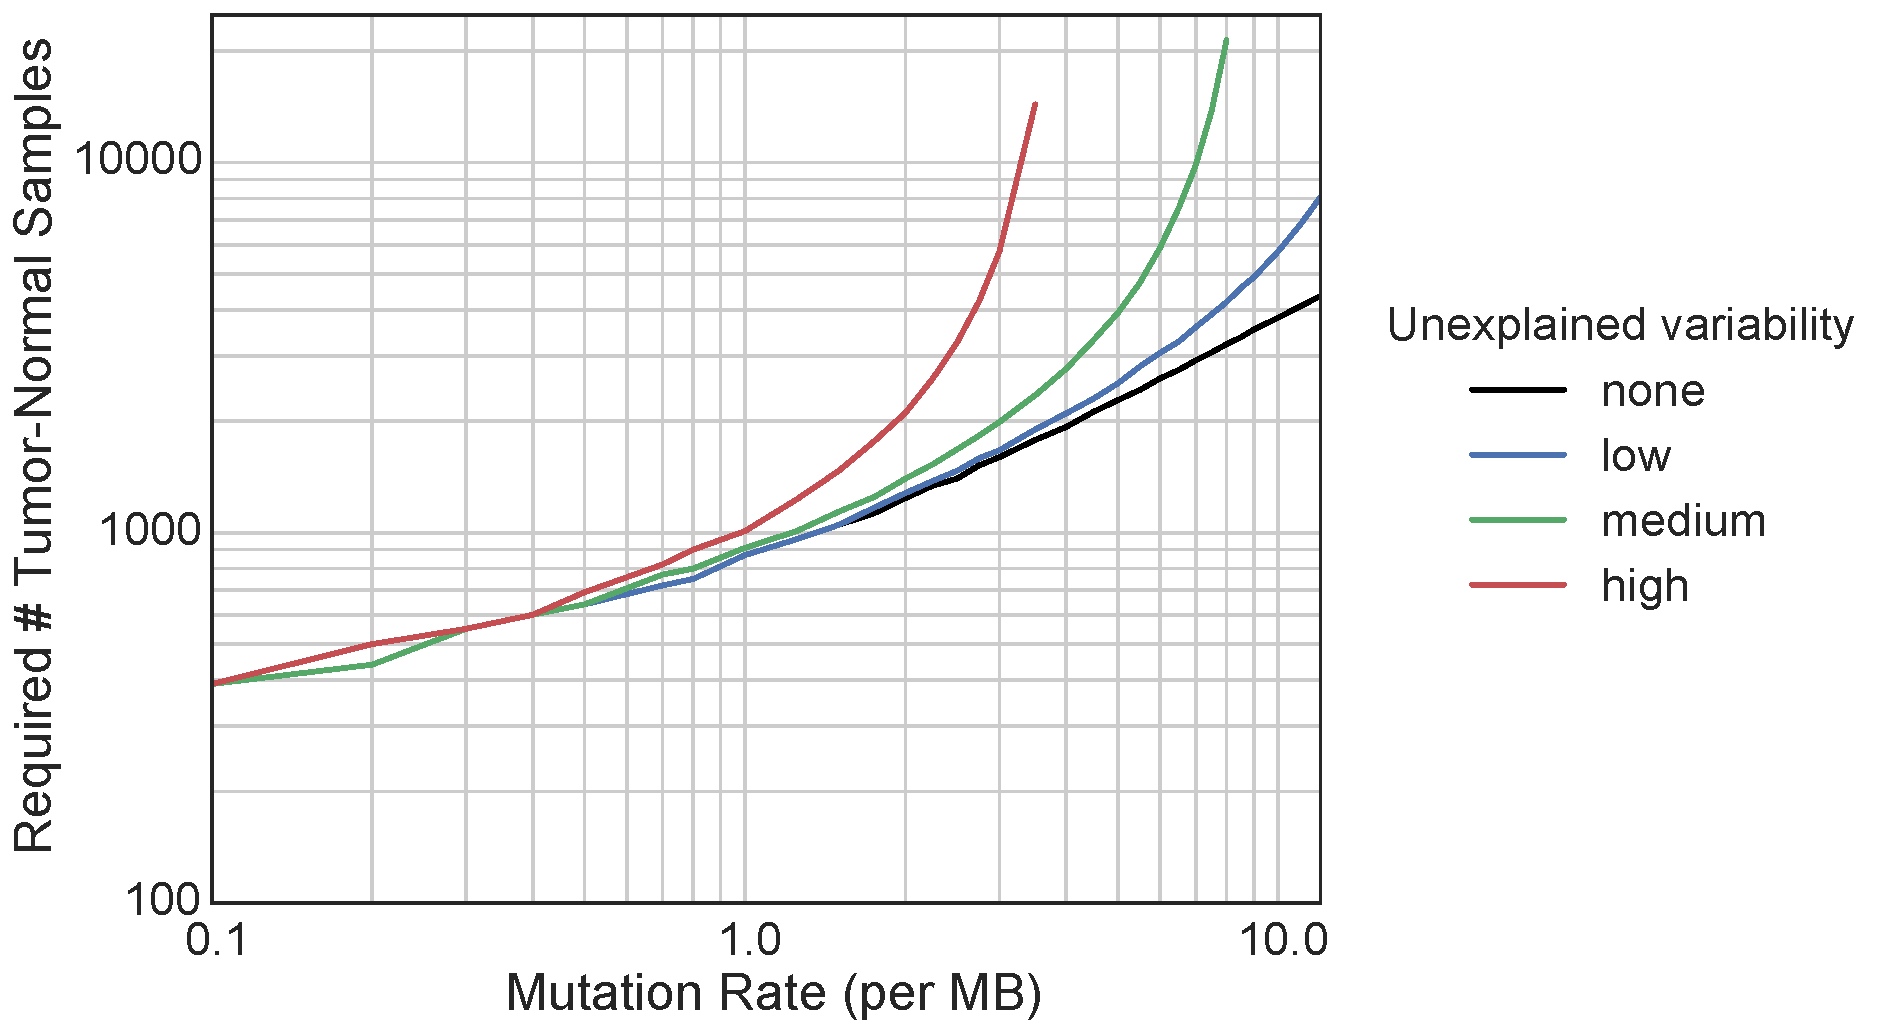
\includegraphics[width=0.9\linewidth]{figures/chapter2/statistical_power.pdf}
  \caption[Sample size required for near-comprehensive detection of driver genes]{Sample size required for near-comprehensive detection of intermediate-effect driver genes (90\% detection and 2\% effect size/increase with respect to background). Results are shown for scenarios with no unexplained variability (black), low (blue), medium (green), and high (red) unexplained variability (CVs of 0.0, 0.05, 0.1, and 0.2, respectively). The number of required samples for the mutation rate-based method becomes very large for moderate-to-high mutation rates and levels of unexplained variability.}
  \label{fig:statistical_power}
\end{figure}

\subsection{Statistical models of mutation rate}

Now I will describe the implementation of the statistical models used to evaluate the effects of unexplained variability in the mutation rate on false positives and statistical power. The first model assumes a correctly estimated background mutation rate μ for a particular gene (binomial model) and the second model assumes that gene background mutation rate varies around μ (beta-binomial model). I used a binomial model similar to previously developed for driver gene power analysis \cite{RN14}. The gene-specific mutation rate factor $F_g$ calculated by MutsigCV \cite{RN14} was set to represent a gene at the 90th percentile, given an exome-wide background mutation rate of π, so that $μ=F_gπ$ ($F_g$ = 3.9). Average gene length ($L$) was set to 1,500 bases and 3/4 mutations were assumed to be non-silent. Effective gene length for non-silent mutations was therefore adjusted as $L_{eff}=3/4L$. Gene background mutation rate was calculated using the total number of potentially mutated bases that could yield a non-silent mutation ($N_{eff}$), which is the effective gene length multiplied by number of samples ($S$). A predicted driver was defined as a gene with significantly higher non-silent mutation rate per base than that gene's background mutation rate, where non-silent mutation rate per base is the following:

\begin{equation}
\mu^{es} = 1 - ((1-\mu)^{L_{eff}}-r)^{1/L_{eff}}
\end{equation}

and $r$ is the fraction of samples with non-silent mutations in the gene above background. Exome-wide background mutation rates of ($\pi$ = 0.5e-6, 3e-6, or 10e-6) were considered.

The beta-binomial was designed to model several levels of unexplained variability around μ. To parameterize the beta-binomial with low, medium, and high variability levels, I used different coefficients of variation (CVs) for the mutation rate (0.05, 0.1, 0.2). Beta-binomial $\alpha$ and $\beta$ parameters were computed as follows:

\begin{equation}
\alpha = \mu\left(\frac{\mu(1-\mu)}{(CV*\mu)^2}-1\right)
\end{equation}
\begin{equation}
\beta = (1-\mu)\left(\frac{\mu(1-\mu)}{(CV*\mu)^2}-1\right)
\end{equation}

To compute the number of false positives expected from a binomial model when unexplained variability is present, I examined the probability that the number of mutations in a gene from a beta-binomial model ($K_{bb}$) would meet or exceed the critical value (for a genome-wide significant driver gene at $\alpha$ = 5e-6) by the binomial, $k'_b$:

\begin{equation}
E[FP] = g*P_{\mu,N_{eff}}[K_{bb}\geq k'_b]
\end{equation}

where $g$ is the total number of human genes (assumed 18,500) and both models use the same mean mutation rate $\mu$ and total number of potentially mutated bases $N_{eff}$.

A similar model is applicable to the effect of various levels of unexplained variability in mutation rate on the power to detect driver genes. I reproduced the binomial model power analysis of \cite{RN14} to estimate the number of samples required for 90\% power to detect genes in the 90th percentile of gene-specific background rate, with 2\% mutation rate above background ($r$ = 0.02). Using Eqs. S3 and S4 to parameterize the beta-binomial model, I calculated the number of samples required for 90\% power at a Bonferroni genome-wide significance level of 5e-6. Samples were iteratively added until there was greater than or equal to 90\% probability that a driver gene with mutation rate μes would be found significant. Because of the jagged power curve for discrete data \cite{RN75}, I found the minimum number of samples required to achieve 90\% power.

\section{A Monte Carlo simulation approach}
\label{sec:monte_carlo}

\subsection{Implementation}

Given the previously highlighted limitations of using the mutation rate, I decided to instead model ratiometric features and statistically condition on the total number of mutations within a gene. This strategy tries to limit the effect of nuisance factors influencing mutation rate that are not always measured or known. Briefly, for each gene, single nucleotide somatic mutations were moved with uniform probability to any matching position in the gene sequence, holding the total number of single nucleotide somatic mutations fixed (Fig. 5). A matching position was required to have the same nucleotide base context (C*pG, CpG*, TpC*, G*pA, A, C, G, T) as the observed position. This method of generating a null distribution controls for the particular gene sequence, gene length, and mutation base context. The number of somatic mutations remains the same, but the mutation consequence of a somatic mutation may change. For example, a somatic mutation that generates a missense mutation may generate a nonsense mutation in its new position. Since mutations that result in insertions and deletions will not change their mutation consequence type by being randomly moved to another position in the same gene, they were moved to a random position in a different gene. This gene was selected based on a multinomial model, with probability proportional to the coding DNA sequence length of the originating gene.

The simulated mutations allow calculating the statistical significance of an arbitrary test statistic computed from the mutation data. Let's say there is a function $T$ of some set of mutation(s) $M$. I can then compute an estimated p-value based on the simulated mutations $M^0$ as follows,

\begin{equation}
\hat{P(M)} = \frac{\#\{T(M^0_i) : T(M^0_i) \geq T(M), i \in 1..S\}}{\#\{T(M^0_i) : i \in 1..S\}}
\end{equation}

where $\hat{P(M)}$ is the estimated p-value and $S$ is the total number of simulations. 

\subsection{Comparison to simulations in CHASM}

There are several notable differences between my implemented Monte Carlo simulation procedure and that previously employed by the method Cancer-specific High-throughput Annotation of Somatic Mutations (CHASM) \cite{RN29}. First, mutations are simulated in a cohort-level manner, rather than considering each unique mutation in isolation. This allows computation of test statistics that may be a function of many mutations found in a single region, a single gene, or in multiple genes. Second, the original CHASM simulations assumed a background rate for mutations at certain nucleotide contexts (termed 'passenger tables'). Instead, I condition on the observed nucleotide context and randomly select another position with the same context. Third, I do not assume a homogenous mutation rate for single nucleotide mutations in genes across the genome. Fourth, my Monte Carlo simulations also apply to all coding mutations, rather than just missense mutations. Lastly, because driver genes may also contain passenger mutations, I do not blacklist simulated mutations in driver genes.

\subsection{Application to salivary gland adenoid cystic carcinoma (ACC)}

\subsubsection{ACC overview}

As part of the statistical analysis, I analyzed coding mutations from 25 whole-genome sequenced Adenoid Cystic Carcinomas (ACC) \cite{RN76}. Specifically, it was noticed that several chromatin regulator genes had more than one non-silent mutation. The question was whether these chromatin regulator genes had a high proportion of truncating mutations, suggesting that they could be tumor suppressor genes.

\subsubsection{Model of truncating point mutations}

I performed a randomization-based statistical test of increased proportion of truncating mutations ($K$) out of total non-silent mutations ($N$) for genes involved in chromatin regulation, controlling for the effect of gene sequence and mutational context. For each gene $i$, our test statistic was

\begin{equation}
T_i = \frac{\#\{t : t\in K\}}{|N|}, where K\subset N
\end{equation}

Truncating mutations were defined as any nonsense, conserved di-nucleotide splice-site mutations, or out-of-frame insertions/deletions (frameshift). Monte Carlo simulations were performed to approximate the null probability distribution of the test statistic $T_i$. Because frameshift mutations do not change consequence when moved to a different position, in the Monte Carlo sample, they were retained with probability equal to the observed proportion of frameshift mutations out of all mutations (maximum likelihood estimate), otherwise they were changed to a non-truncating mutation. After each iteration of this sampling procedure, the number of mutations in a gene is always the same, but the mutation consequence of each mutation may change. Thus, the test statistic $T_i$ for the gene will change values at each iteration, and repeated iterations yield a null distribution of test statistics to estimate the P value of the gene's observed test statistic. For the gene group analysis, my test statistic was

\begin{equation}
T_c = \frac{\sum_{i\in c}{\#\{t:t\in K_i\}}}{\sum_{i\in c}{|N_i|}}
\end{equation}

and it was computed both for the observed and simulated mutations. A one-tailed empirical P value was calculated as the fraction of Monte Carlo samples in which the observed value of the test statistic was equal to or higher than the simulated value. Increasing the number of iterations of Monte Carlo sampling increases the precision of the P value; 10,000,000 iterations were
chosen to achieve adequate precision.

\subsubsection{Results}

Several genes with well-known roles in chromatin regulation were mutated in multiple tumors: MLL2, MLL3, EP300, SMARCA2, SMARCC1, and KDM6A. The proportion of truncating mutations (nonsense codons, splice-site alterations, or out of-frame insertions and deletions) out of the total number of non-silent mutations in these genes was high (6 of 11), significantly greater than expected by chance (P = 3.8e-6). Furthermore, MLL2 and EP300, when considered individually, had a significantly higher proportion of truncating mutations than expected by chance (P = 0.008 for MLL2 and P = 0.01 for EP300). This finding is consistent with the hypothesis that several of these genes played an important role in the cancers in which they occurred.

\section{Conclusions}

The goal in this chapter was to first understand "how" somatic mutations accumulate in the absence of selection so as to, later, correctly interpret "which" mutations are cancer drivers in the presence of positive selection. A recent study indicates there is limited purifying selection of point mutations in cancer \cite{RN56}, suggesting the lack of incorporating negative selection in statistical models is not a major concern. I have shown in this chapter that background mutation rate is highly variable at multiple scales and therefore is difficult to statistically model. This can either lead to increased false positives or reduced statistical power when attempting to identify cancer driver genes. However, many of the known covariates modulate mutation rate at the scale of megabases within the genome \cite{RN74}, but nearly all genes span $<$1MB. I therefore developed Monte Carlo simulations to test any arbitrary test statistic by conditioning on the total number of mutations within a gene while accounting for nucleotide sequence context. The flexibility of the Monte Carlo simulations will be critical in later chapters when evaluating the significance of results from machine learning methods. 
%!TEX root = root.tex

\chapter{20/20+: a machine learning method to predict cancer driver genes}
\label{chap:ch3}
\chaptermark{20/20+}

\section{Introduction}

The first exomic analyses attempted to identify candidate driver genes as those having more mutations than expected from some presumed background somatic mutation rate, corrected for base context, gene size, and other variables \cite{RN78, RN4}. Subsequent work has considerably refined the variables involved in determining whether a gene is more mutated in cancers than expected by chance. This has led to a variety of "significantly mutated gene" methods that adjust for covariates such as replication timing and gene expression as well as including more sophisticated metrics of mutational base contexts \cite{RN13, RN43}. Although methods have been extended to utilize gene expression \cite{RN80, RN84, RN81, RN83, RN79, RN82}, I will focus solely on driver gene analysis based on somatic point mutations.

An alternative method to finding cancer drivers employs a ratiometric approach. Rather than attempting to determine whether the observed mutation rate of a gene in cancers is higher than expected by chance, these methods simply assess the composition of mutations normalized by the total mutations in a gene. The ratiometric 20/20 rule \cite{RN25} evaluates the proportion of inactivating mutation and recurrent missense mutations in a gene of interest. Other ratiometric approaches use mutation functional impact bias \cite{RN86, RN53}, mutational clustering patterns \cite{RN87, RN54, RN71}, or patterns of mutation composition \cite{RN71}. Here, I describe a machine-learning-based, ratiometric method (20/20+) that formalizes and extends the original 20/20 rule and enables automated integration of multiple features of positive selection.

\section{Original 20/20 rule}

The original 20/20 rule was a manually designed set of decision rules to identify cancer driver genes as either an oncogene or tumor suppressor gene (\autoref{fig:2020rule}) \cite{RN25}. The name derives from the rule that oncogenes should have at least 20\% of mutations being recurrent (observed more than once) and tumor suppressor genes should have at least 20\% inactivating mutations (i.e., frame shift indels, nonsense mutations, etc.). In addition, there are count thresholds that are specifically tuned for analyzing a specific version of the COSMIC database \cite{RN95}. When I applied this rule to a later version of COSMIC, it had inadequate specificity (data not shown). Moreover, scaling the count thresholds relative to database size also produced similar results, suggesting additional manual curation of results would be necessary. Consistent with this observation, the 20/20 rule had good performance at distinguishing oncogenes versus tumor suppressor genes within already pre-defined driver genes \cite{RN88}.

\begin{figure}
  \centering
  \makeatletter
  \let\@currsize\normalsize
  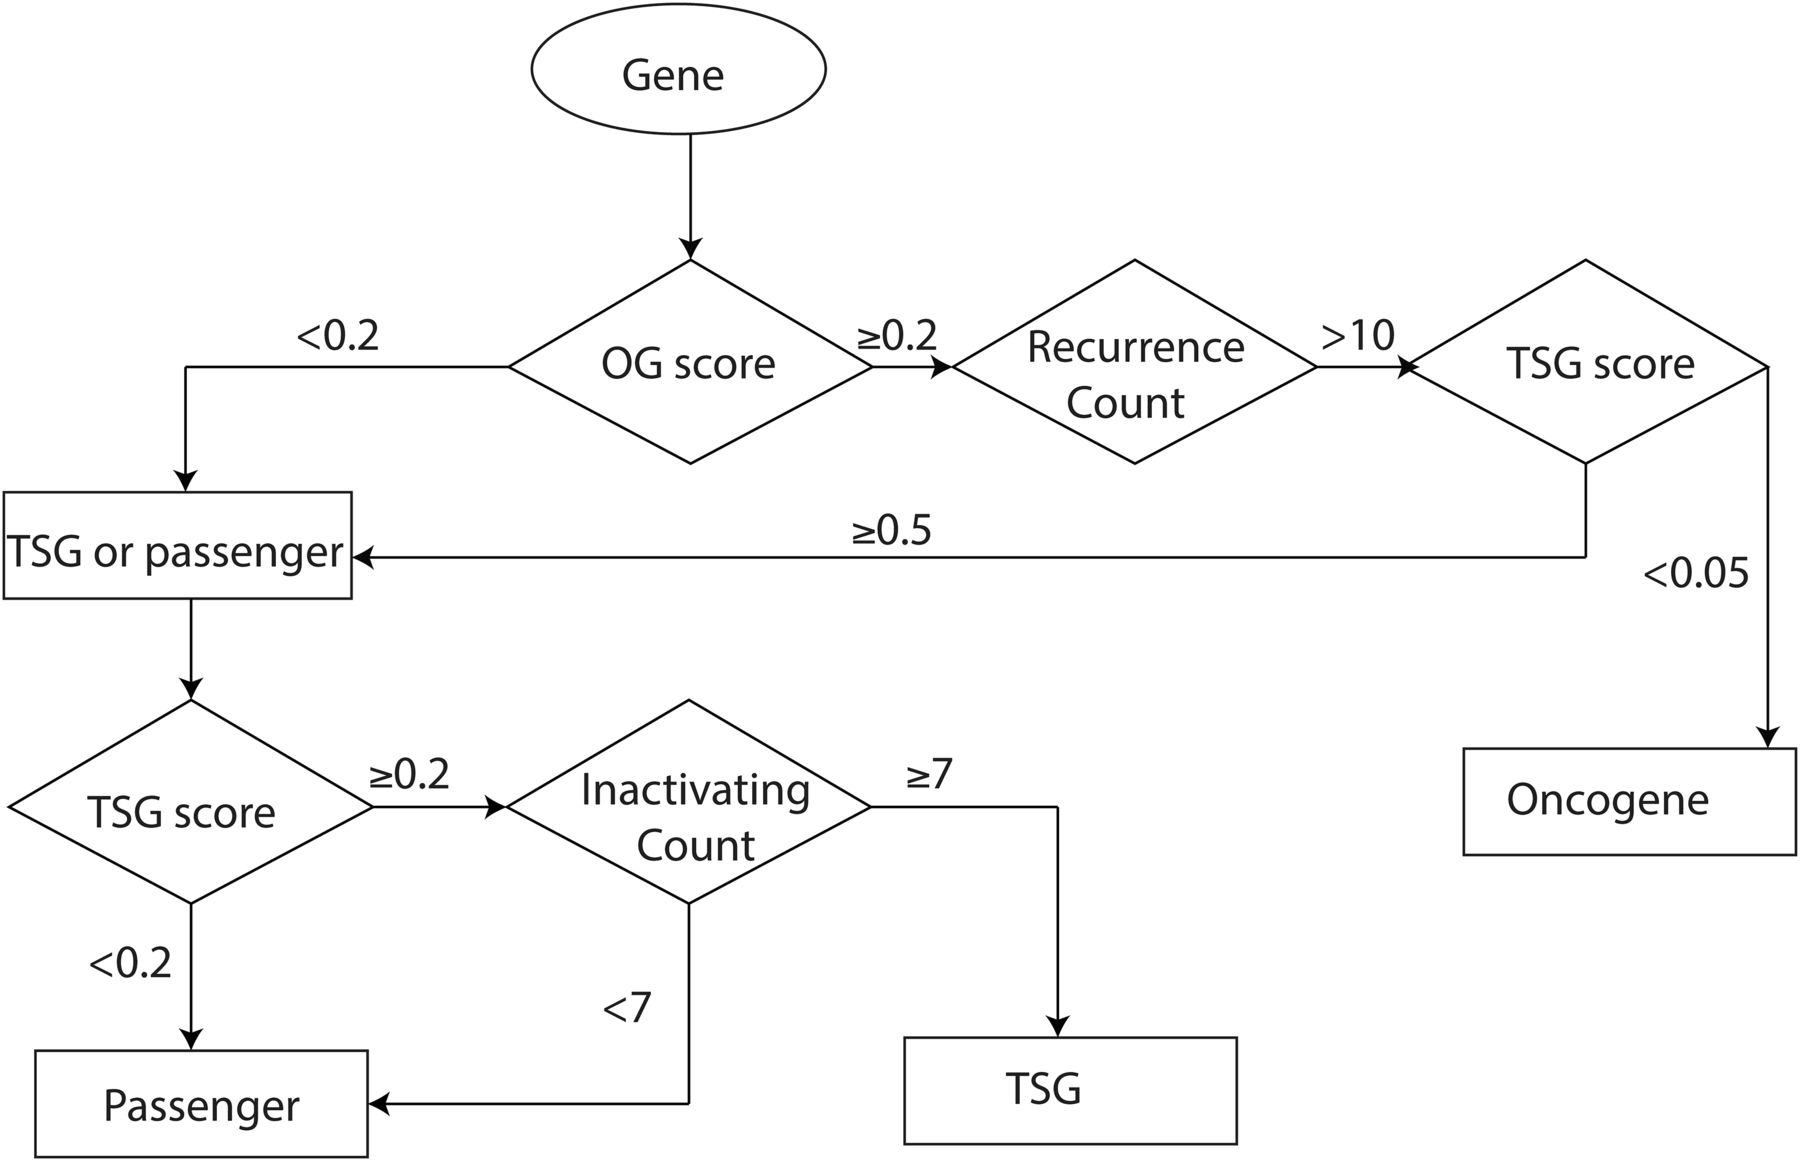
\includegraphics[width=0.9\linewidth]{figures/chapter3/2020_rule.jpg}
  \caption[Decision tree underlying 20/20 rule.]{Decision tree underlying 20/20 rule. Each gene is input into the tree and oncogene (OG) and tumor suppressor gene (TSG) score computed. Thresholds of each score and the numerator of the OG score (recurrence count) and TSG score (inactivating count) are used to determine whether a gene is an OG, TSG, or passenger.}
  \label{fig:2020rule}
\end{figure}

\section{Machine learning prediction of cancer driver genes}

Using machine learning, 20/20+ trains a random forest to leverage many features simultaneously to predict cancer driver genes. Random forests outperformed logistic regression, boosting, and support vector machines (data not shown). I will first go over the mathematical background of random forests and then describe the implementation in 20/20+.

\subsection{Mathematical overview of random forests}

\subsubsection{Decision tree}

Since my focus will be on classification, a decision tree $\pi(X)$ will return 1 if the prediction is a cancer driver and 0 for a passenger. A decision tree is constructed from a set of possible questions $Q=\{Q_1,…,Q_N\}$, with a question taking the following form,

\begin{equation}
Q_.(X)=I_{X_i \leq c}
\end{equation}

where $I$ is the indicator function, $X_i$ is the i'th feature value, and $c$ is a constant. The question asked by a decision tree depends on the previous question asked. To keep track of order of questions, the index of the first question will be denoted $\rho_1$, where $\rho_1∈\{1…N\}$. The second question will therefore be a function of the answer from the first question, $\rho_2=\rho_2(a_1)$, where $a_1=Q_{\rho_1}$. More generally there is a series of questions $\beta_n=\{Q_{\rho_1}=a_1,…,Q_{\rho_{n-1}}=a_{n-1}\}$ prior to the n'th question.

Each question will split training examples depending on the answer to the question. The goal of the decision tree is to utilize questions that reduce the uncertainty in the distribution of class labels. I will regard the distribution of class labels as the probability of observing a class label given the answer to a question n as follows,

\begin{equation}
p_k=Pr⁡(Y=1|Q_{ρ_n}=k,\beta_n)
\end{equation}

where $k$ is the answer to the question and $p_k$ is the proportion of labeled drivers. For the decision tree algorithm, the best question defined by the gini impurity is used at each step:

\begin{equation}
\rho_n=\argmin_{1 \leq b \leq N}{2\sum_{k=0}^{1}{Pr[Q_b=k]p_k(1-p_k)}}
\end{equation}

There are various practical criteria to decide when to stop asking further questions in a decision tree, but I will not cover this here. Assuming a decision tree is constructed, the predicted class is chosen by the most likely class following the terminal question.

\begin{equation}
\pi(X) = \argmax_l{Pr(Y=l|\beta_*)}
\end{equation}

where $l\in \{0,1\}$ is the class label and $\beta_*$ contains the history of answers for all questions. 

\subsubsection{Random Forest}

A random forest is an ensemble of many randomized decision trees \cite{RN41, RN40}, where each tree is trained on a random selection of training set examples and candidate features, via a recursive splitting process \cite{RN89}. This involves constructing each tree $\pi_j$ from a bootstrapped sample of the training data $D_j=\{(X(i),Y(i)),…\}_{i=1..m}$. Then instead of allowing all questions for each split, a random subset of questions is used $Q^s\subset Q$, were the number of features $s$ is usually taken to be proportional to the square root of the total features p,  $|s|=\sqrt{p}$. Lastly, once $J$ decision trees are constructed, random forest predictions result in a score between 0 and 1 that reflects the proportion of trees agreeing with the class label of cancer driver:

\begin{equation}
f(X) = \frac{1}{J}\sum_{j=1}^J{\pi_j(X)}
\end{equation}

\subsection{Random Forest implementation}

Although the above mathematical description of a random forest was in terms of two classes (drivers and passengers) for simplicity, random forest classification also extends to multi-class classification. 20/20+ uses a three-class classifier which predicts a gene as either an oncogene, tumor suppressor genes, or passenger gene. I used the set of oncogenes and tumor suppressor genes identified by the original 20/20 rule as a training set \cite{RN25}. Considering cancer driver genes (oncogenes or tumor suppressor genes) constitute only a small proportion of all genes, I labeled all other genes as passenger for the purpose of training. 

\subsubsection{Features}

I designed a set of 24 predictive features described in \autoref{table:feature_tab} and whose feature importance is shown in \autoref{fig:2020features}, as assessed by the mean decrease in gini impurity. Many of the features are components of the 20/20 rule OG and TSG scores, and I included several ratiometric features not in the original 20/20 rule, for example, ratio of missense to silent mutations, as well as features that represented mutation functional impact and gene importance. Normalized missense entropy, a measure of positional clustering, was calculated as follows:

\begin{equation}
E_k = \frac{\sum_i{p_i\log_2{p_i}}}{\log_2{k}}
\end{equation}

where $k$ is the total number of missense mutations in a gene and $p_i$ = (count of missense mutations in the I'th codon)/k. Three of the 24 features represented p-values and were calculated using the monte carlo simulation described in \autoref{sec:monte_carlo}.

\begin{figure}
  \centering
  \makeatletter
  \let\@currsize\normalsize
  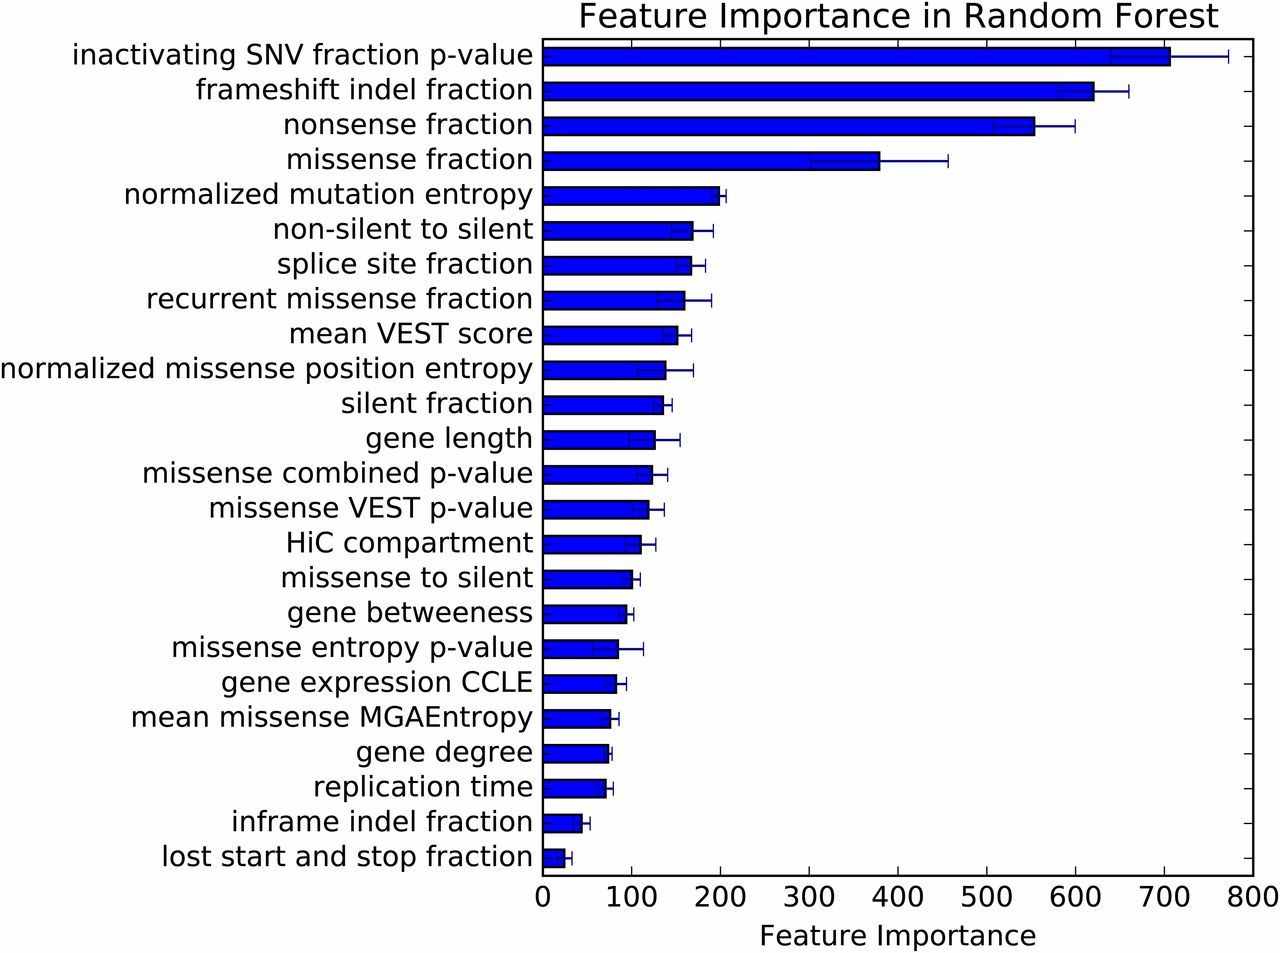
\includegraphics[width=0.9\linewidth]{figures/chapter3/feature_importance.jpg}
  \caption[Random Forest feature importance ranking for the 24 predictive features.]{Random Forest feature importance ranking for the 24 predictive features. The mean decrease in Gini index is plotted for each feature. Error bars indicate SD when feature importance calculation was repeated on 10 different cross-validation partitions. CCLE, Cancer Cell Line Encyclopedia \cite{RN13}; HiC, 3D chromatin interaction capture \cite{RN13}; MGAEntropy, Shannon entropy in column of a vertebrate genome 46-way alignment corresponding to location of the mutation \cite{RN90}; SNV, single-nucleotide variant; VEST, Variant Effect Scoring Tool \cite{RN30}.}
  \label{fig:2020features}
\end{figure}

\subsubsection{Handling class imbalance}

With only 54 OGs and 71 TSGs labeled by the original 20/20 rule, the number of passenger genes far exceeds the number of labeled driver genes, creating a problematic class imbalance \cite{RN93}. I use a subsampling approach, previously recommended for random forests \cite{RN92}, in which for my case the passenger genes are sampled at a 1:1 ratio to OGs plus TSGs. To compensate for the remaining OG and TSG imbalance, the Random Forest is trained with class weights inversely proportional to the sampled frequency of the class. Predictions were made with a random forest of 200 trees. The number of trees only had minor impact on the overall performance. I used 10-fold gene hold-out cross-validation to avoid overfitting. The procedure of 10-fold cross-validation was repeated five times (1,000 trees in total), and the resulting scores from each gene were aggregated to limit minor fluctuations in scores due to randomization in the cross-validation folds.

\subsubsection{Random forest prediction}

Each gene was scored as the fraction of trees that voted for oncogene, tumor suppressor gene, or passenger gene. A driver score for each was calculated as the sum of the oncogene and tumor suppressor gene scores. A driver score was included in case the gene was likely a cancer driver, but the precise type of cancer driver gene was hard to determine.

\section{Statistical significance}

The statistical significance of each gene score was computed with an extension of the Monte Carlo simulation algorithm described in \autoref{sec:monte_carlo}. For each gene, the Monte Carlo simulation was repeated 10 times, and for each simulation all 24 features were computed. In this process, protein interaction network features (degree and betweenness) were, additionally, permuted as a pair. The features of gene length, replication timing, HiC value, and average Cancer Cell Line Encyclopedia (CCLE) gene expression were not altered. Next, each "simulated" gene was scored with the Random Forest previously trained on the real data. The resulting OG, TSG, and driver scores for all simulated genes were used as an empirical null distribution. To compute a P value for a gene score, I used the fraction of simulated genes with a score equal to or greater than the score. P values were adjusted by the Benjamini-Hochberg method \cite{RN94} for multiple hypotheses. I compute a Benjamini-Hochberg q-value as follows,

\begin{equation}
q(i) = \min{\left(\min_{i..n}{\frac{p(i)}{i/n}}, 1 \right)}
\end{equation}

where $p(i)$ is the i'th smallest p-value, $q(i)$ is the corresponding q-value, n is the total number of p-values, and the cumulative minimum from index n to i. Consistent with other driver gene prediction methods, I considered a gene to be significant ($q \leq 0.1$) if any of the OG, TSG, or driver scores were significant. The strategy of converting p-values to q-values is for convenience and does not change the significant p-values by the procedure originally outlined by Benjamini and Hochberg \cite{RN94}.

\section{Conclusions}

In this chapter, I developed a new method, 20/20+, which addresses two major issues with the original 20/20 rule: use of a limited number of features and a lack of a statistically principled threshold to limit false positives. 20/20+ uses the random forest algorithm to make predictions using a non-linear combination of features. Importantly, 20/20+ uses ratiometric features to normalize artefactual differences between cancer types and regions of the genome. Because Random Forests do not intrinsically include hypothesis testing techniques, I used simulated mutations to assess the statistical significance of scores. P-values were estimated from a simulated null distribution, controlling for sequence composition, and corrected for multiple testing with the Benjamini-Hochberg method \cite{RN94}. The application and benchmarking of 20/20+ will be considered in Chapters 4 and 7.


%!TEX root = root.tex

\chapter{Benchmarking cancer driver gene predictions}
\label{chap:ch4}
\chaptermark{Cancer driver gene benchmark}

Rigorous and unbiased evaluation is necessary to inform users about the comparative utility of prediction methods. In many investigative domains, there is a generally accepted gold standard against which predictions can be benchmarked \cite{RN102, RN103}. However, only a limited number of genes have been fully vetted as cancer drivers. In previous work, driver prediction has been benchmarked by significant overlap with the Cancer Gene Census (CGC) \cite{RN91}, which is a manually curated list of likely but not necessarily validated driver genes \cite{RN54, RN53} or by agreement with a consensus gene list of drivers predicted by multiple methods \cite{RN96}. To our knowledge, a systematic framework for the evaluation of somatic mutations that can be generally applied has not been previously developed. Eight methods were evaluated: MutsigCV \cite{RN13}, ActiveDriver \cite{RN98}, MuSiC \cite{RN43}, OncodriveClust \cite{RN54}, OncodriveFM \cite{RN53}, OncodriveFML \cite{RN86}, Tumor Suppressor and Oncogenes (TUSON) \cite{RN71}, and 20/20+ \cite{RN70}. 

In this chapter, I present a framework for such evaluations. The framework has five components, some of which have been previously applied in isolation, but not as part of a unified system. I considered overlap with CGC, agreement between methods, comparison of observed vs. theoretical P values, number of significant genes predicted, and prediction consistency on independent partitions of the dataset. To implement this framework, I first collected 729,205 published somatic mutations from 34 cancer types \cite{RN14, RN71} \autoref{fig:benchmark_data}. These mutations were composed of single base substitutions and in-frame and out-of-frame insertions and deletions (indels) of less than 10 bp. I then compared various methods on the full pancancer set.

\begin{figure}
  \centering
  \makeatletter
  \let\@currsize\normalsize
  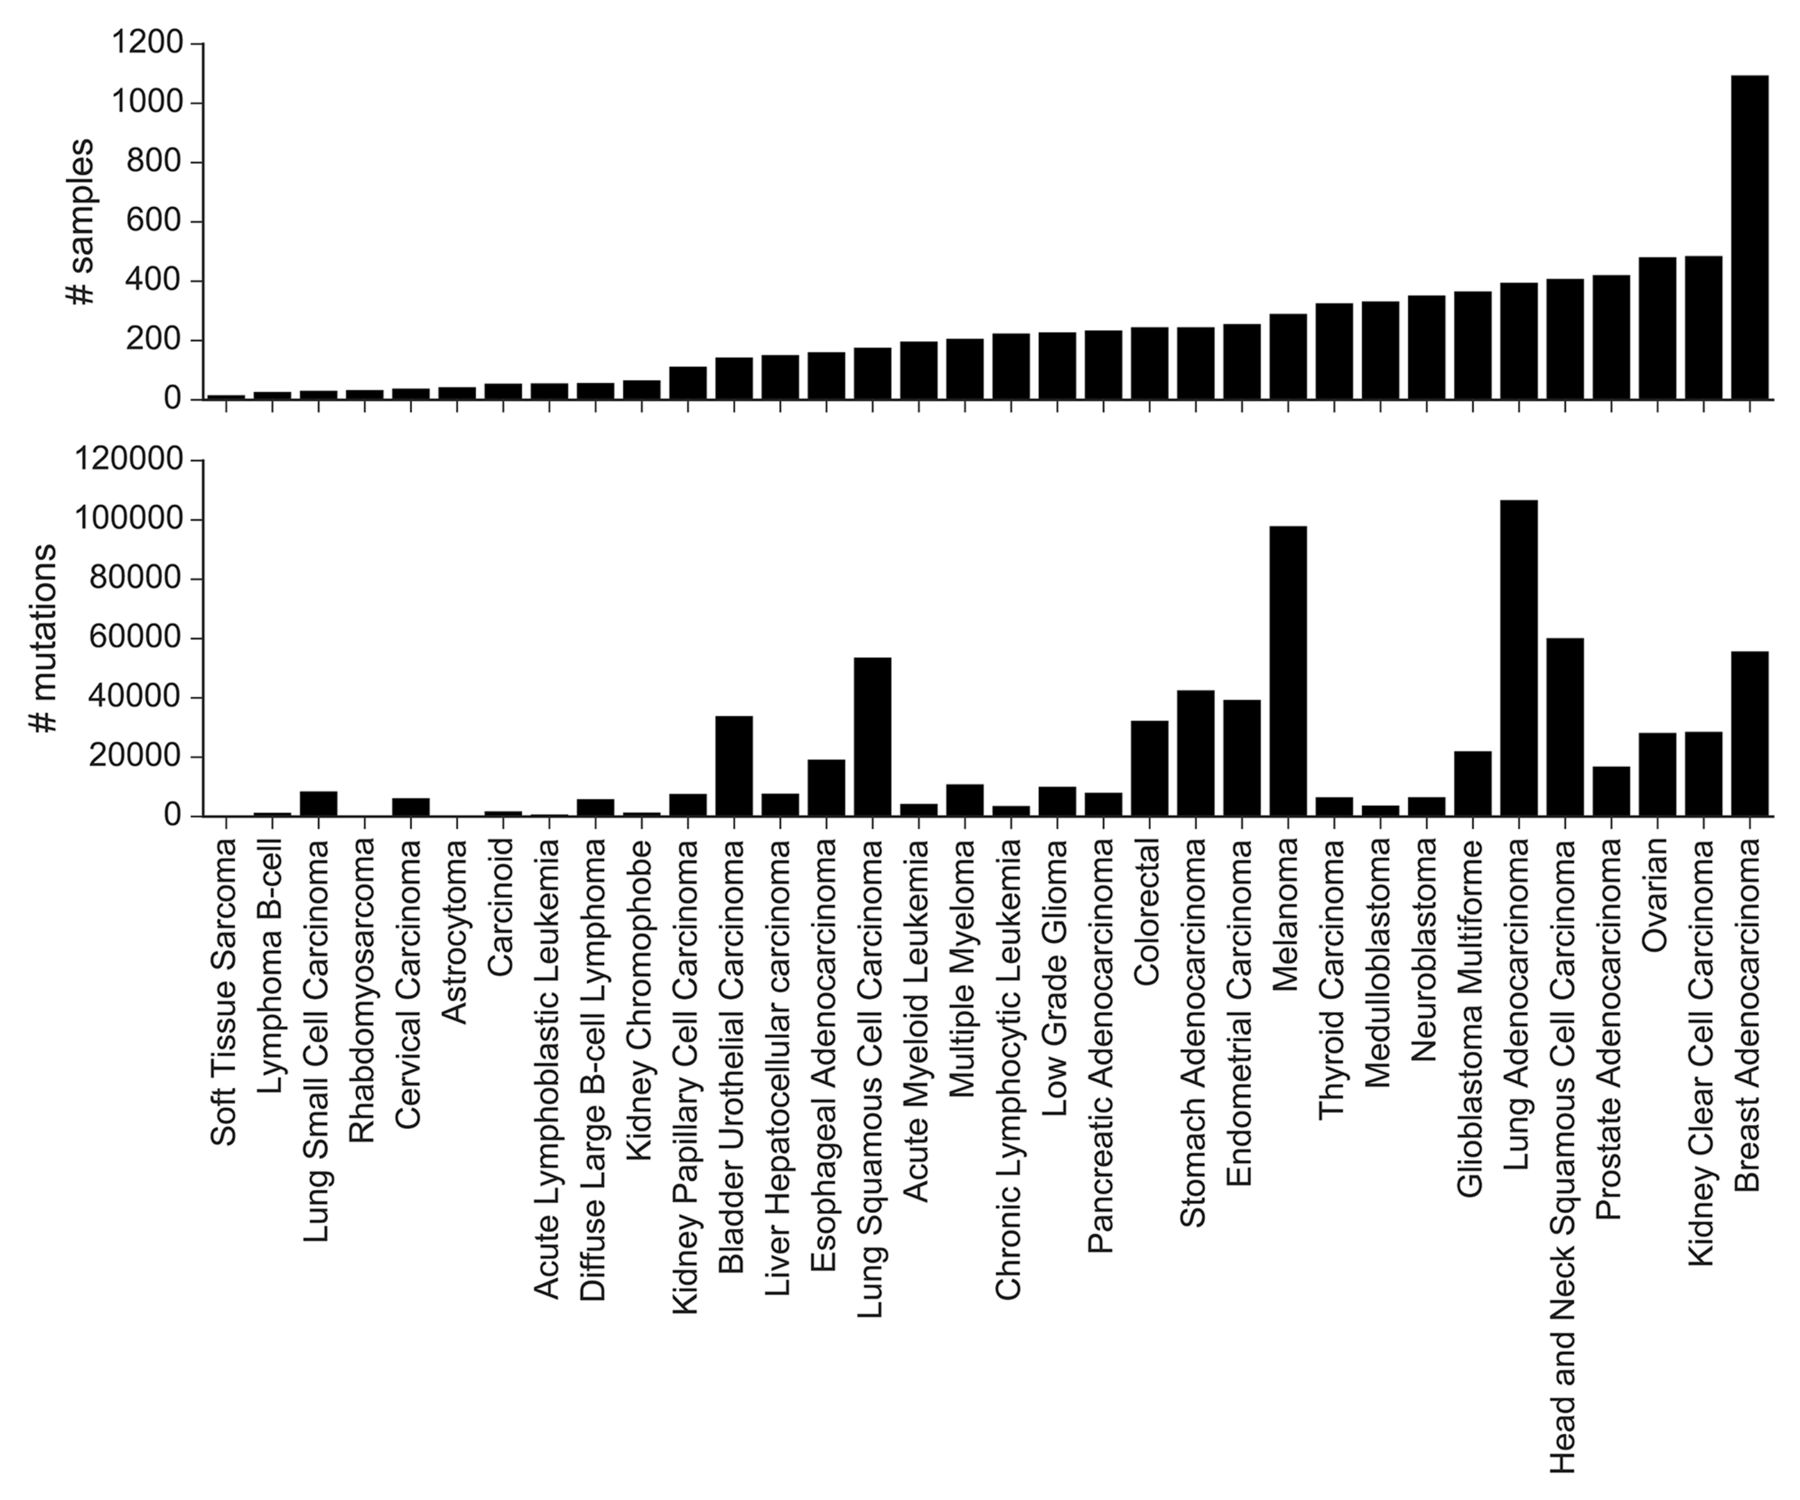
\includegraphics[width=0.9\linewidth]{figures/chapter4/study_size.jpg}
  \caption{Summary of evaluation dataset. The evaluation dataset consisted of mutations spanning 34 cancer types. All included mutations were small somatic variants. Cancer types are ordered from Left to Right by number of samples, ranging from 15 for soft-tissue sarcoma to 1,093 for breast adenocarcinoma, with an average of 232 samples per cancer type. These cancer types span a wide range of solid and several liquid cancers, including multiple tissues and cell types of origin, different background mutation rates, and different numbers of available samples. For each cancer type, total mutations and number of available samples are shown.}
  \label{fig:benchmark_data}
\end{figure}

\section{Overlap of the Driver Genes Predicted by Each Method}

First, I assessed overlap of the predicted driver genes with the CGC. I considered only those CGC genes typed as somatic, missense, frameshift, nonsense or splice site, excluding translocations, large amplifications/deletions, and other mutation consequence types not addressed in our study, yielding a total of 188 CGC genes. Although the driver genes predicted by all methods were enriched for CGC genes, the predicted drivers by any individual method did not contain a majority of CGC genes (\autoref{fig:benchmark_result}A). Three methods (20/20+, MutsigCV, and TUSON) had substantially higher fractions of predicted drivers in the CGC than the other methods. When I considered a subset of 99 CGC genes supported by functional studies \cite{RN99}, the results were very similar. The ranking of methods by fraction predicted was essentially the same as with the full CGC, with the three methods listed above having substantially higher fractions than the rest.

Genes predicted by more than one method may be more likely to be drivers \cite{RN96}. For each method, I calculated the fraction of predicted drivers that were unique or predicted by at least one, two, or three other methods (\autoref{fig:benchmark_method_overlap}). As shown in \autoref{fig:benchmark_method_overlap}, there was little consensus in prediction of driver genes among the methods. The majority (59-80\%) of genes identified by MuSiC, ActiveDriver, OncodriveClust, OncodriveFML, or OncodriveFM were not observed by any of the other seven methods. The fractions of genes identified by TUSON, 20/20+, and MutsigCV that were not identified as driver genes in at least one of the other seven methods was 14\%, 19\%, and 33\%, respectively. Although it is likely that some of the uniquely predicted drivers are bona fide, I could not find convincing literature support for the top-ranked unique predictions of MuSiC, ActiveDriver, and the Oncodrive methods. 

\begin{figure}
  \centering
  \makeatletter
  \let\@currsize\normalsize
  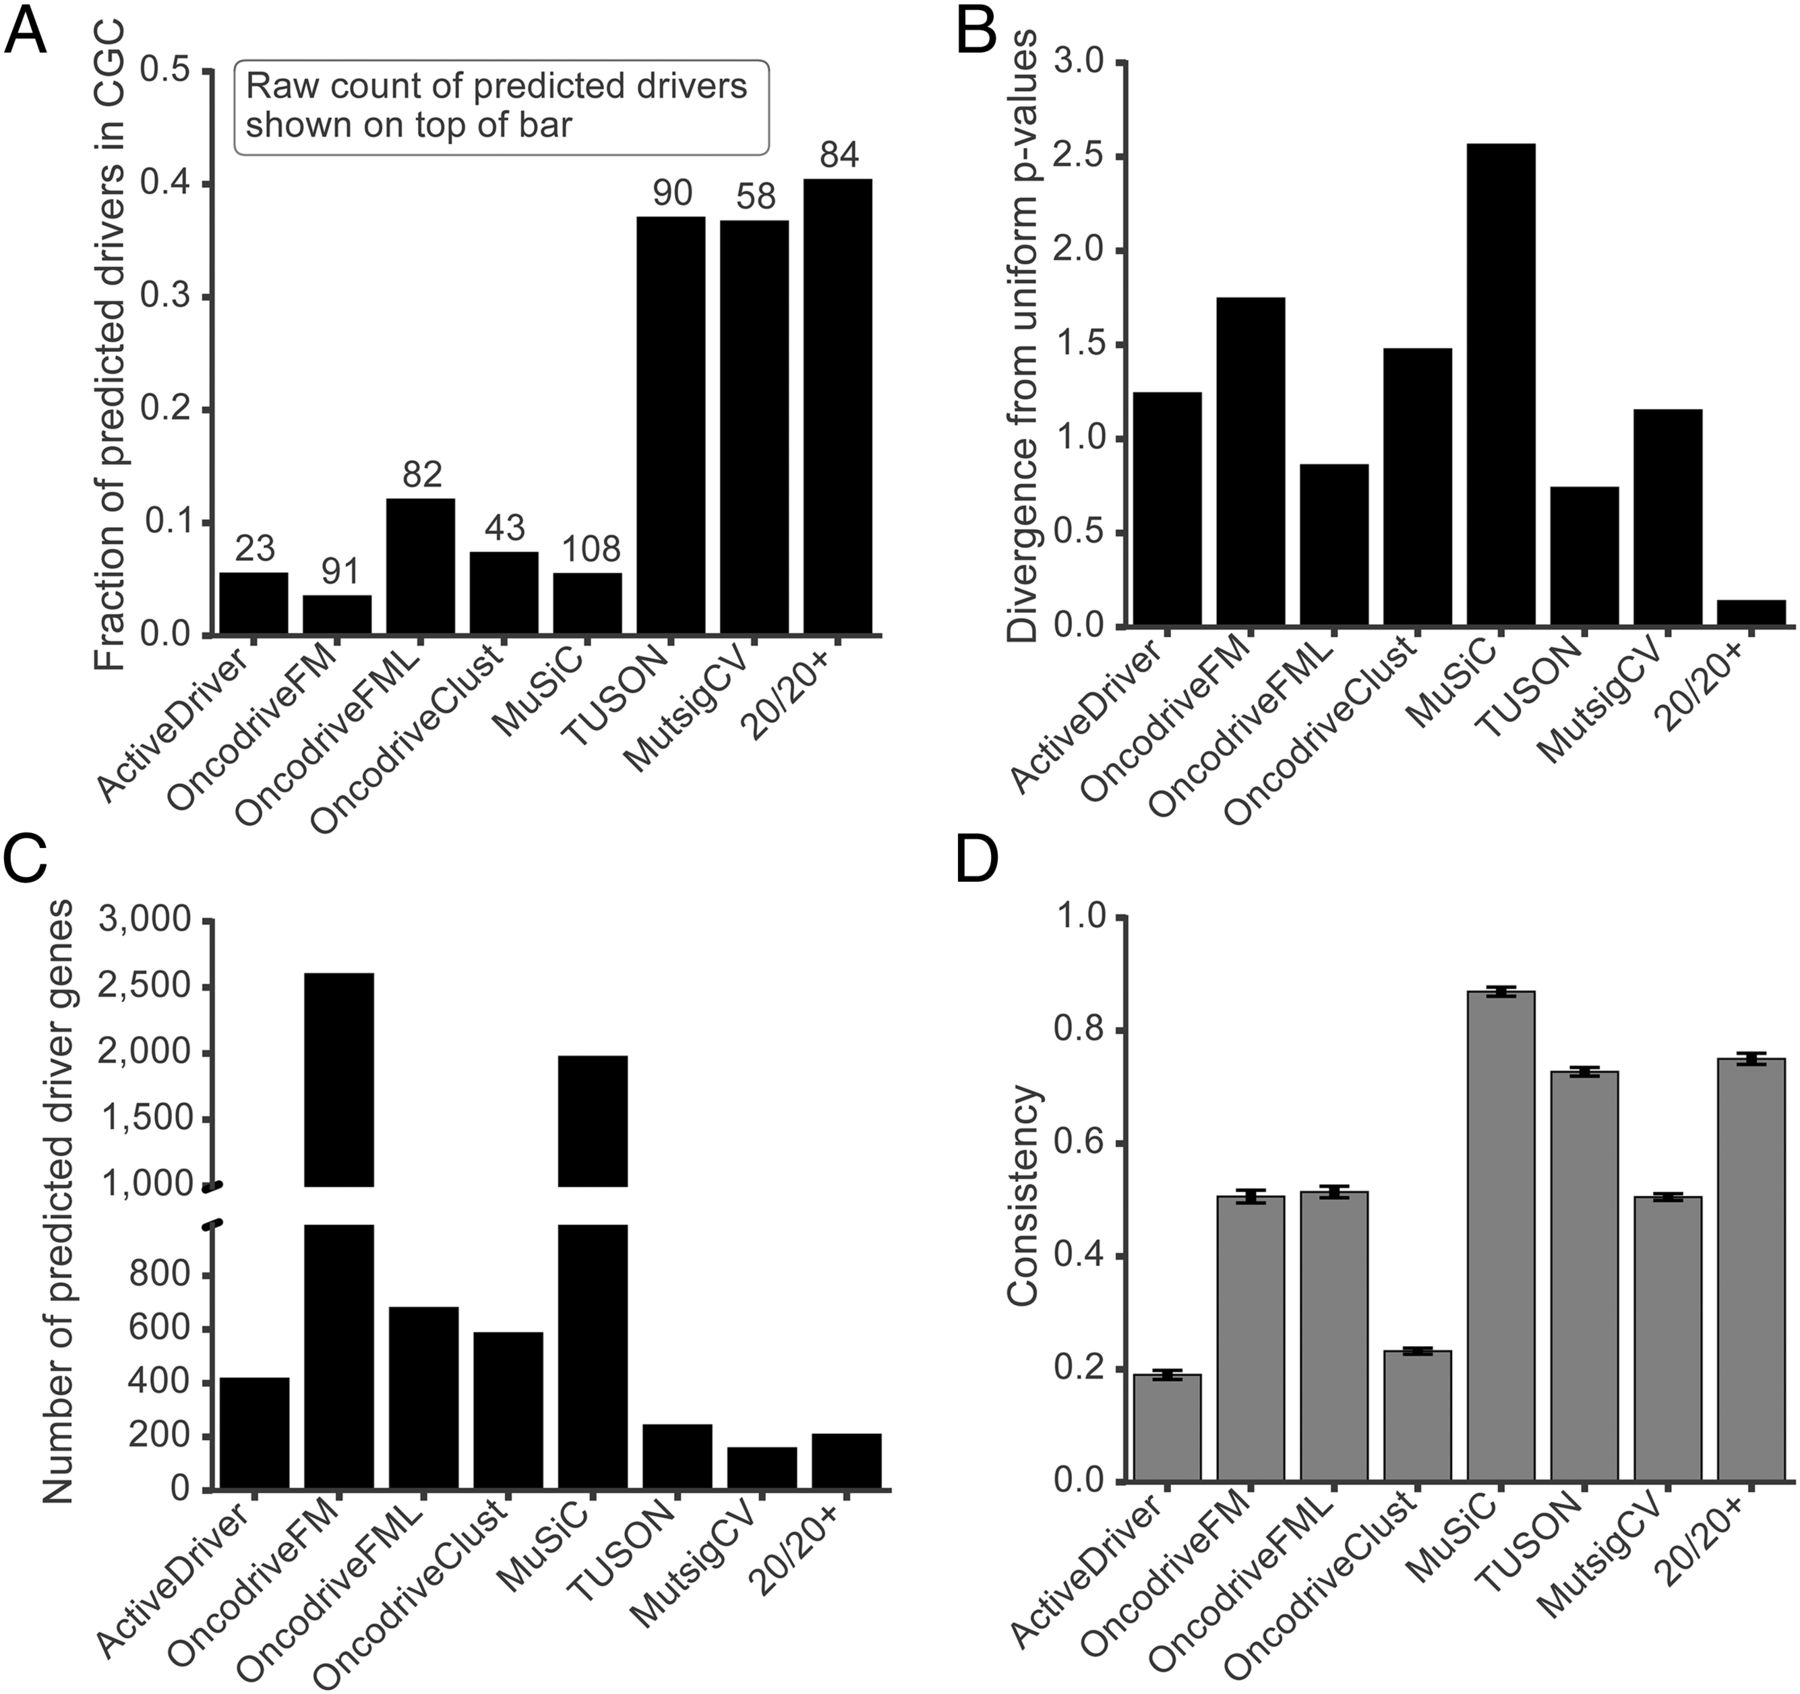
\includegraphics[width=0.9\linewidth]{figures/chapter4/evaluation.jpg}
  \caption{Outputs of eight driver prediction methods run through the evaluation protocol. (A) Fraction of predicted driver genes (q ≤ 0.1) that are found in the Cancer Gene Census (CGC) (downloaded April 1, 2016). Raw count of predicted driver genes indicated on Top of each bar. (B) Divergence from uniform P values, measured as mean log fold change (MLFC) between a method's observed and desired theoretical P values. (C) Number of predicted driver genes. Driver gene is defined as having Benjamini-Hochberg adjusted P value, $q \leq 0.1$. (D) Consistency of each method measured by TopDrop consistency (TDC) at depth of 100 in the method's ranked list of genes. Error bars indicate +/-1 SEM across 10 repeated splits of the data.}
  \label{fig:benchmark_result}
\end{figure}

\begin{figure}
  \centering
  \makeatletter
  \let\@currsize\normalsize
  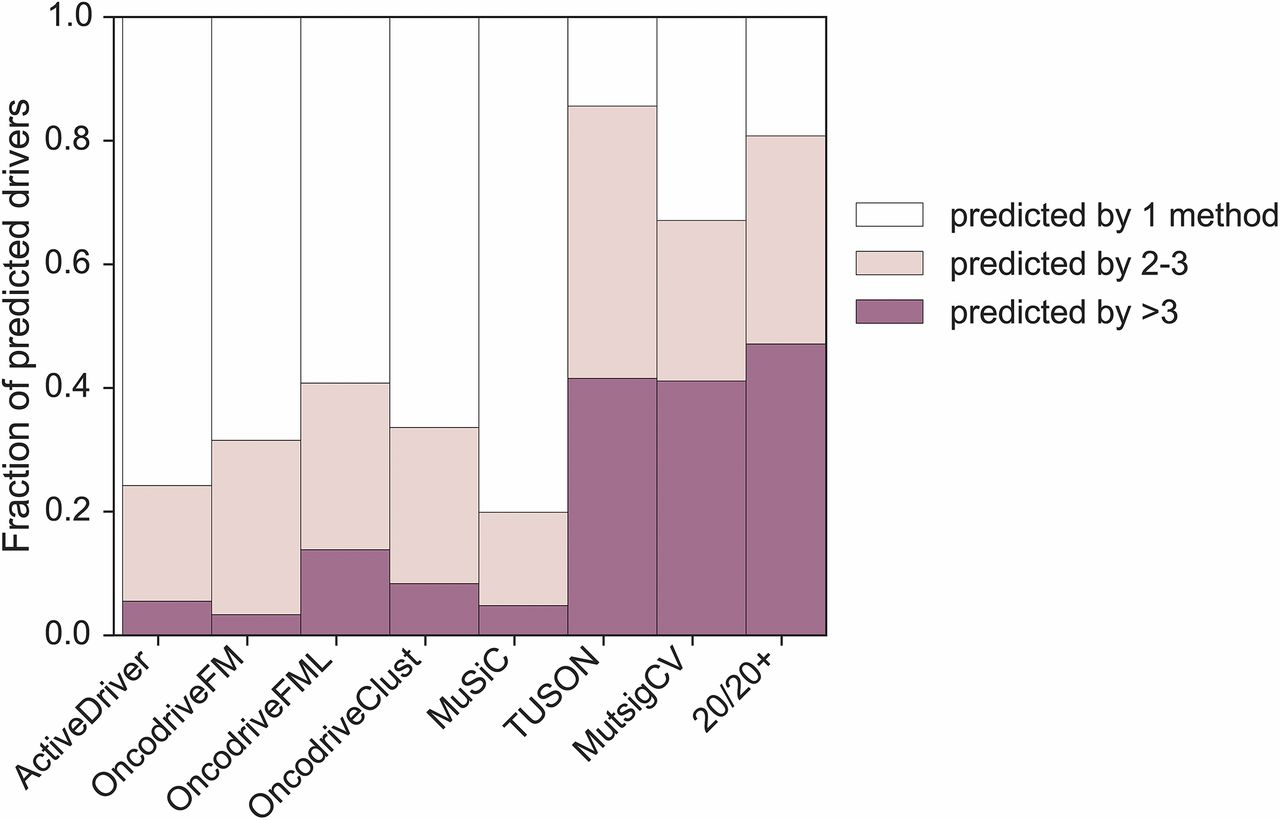
\includegraphics[width=0.9\linewidth]{figures/chapter4/method_overlap.jpg}
  \caption{Fraction of predicted driver genes for each method by consensus among methods. Fraction of predicted drivers unique to each method, predicted by two to three methods or predicted by more than three methods are shown. A predicted driver gene is defined by Benjamini-Hochberg adjusted P value ($q \leq 0.1$)}
  \label{fig:benchmark_method_overlap}
\end{figure}

\section{Observed vs. Expected P Values}

Given the lack of agreement among these various methods, I compared P values reported by each method to those expected theoretically. Such comparisons are often used in statistics and can indicate invalid assumptions or inappropriate heuristics. Theoretically, the P value distribution should be approximately uniform after likely driver genes are removed \cite{RN188}. Therefore, I removed all genes predicted to be drivers by at least three methods after Benjamini-Hochberg multiple-testing correction ($q \leq 0.1$) and any remaining genes in the CGC. I assumed that the number of bona fide driver genes not removed by this procedure would be small enough to have minimal impact on the P value distribution. To quantify the differences between the observed P values and those expected from a uniform distribution, I developed a measure named mean absolute log2 fold change (MLFC) (see \autoref{sec:mlfc_justification}). MLFC values near zero represent the smallest discrepancies and the closest agreement between observed and theoretical P values.

One method (20/20+) had an MLFC that was fivefold lower than the seven others (\autoref{fig:benchmark_result}B). I also compared observed and theoretical P values with quantile-quantile plots, which provide a detailed view of P value behavior (\autoref{fig:qq_plot}A). 20/20+ P values had by far the best agreement with theoretical expectation across the entire range of supported values. In the critical range typically used to assess statistical significance ($P \leq 0.05$), OncodriveClust, OncodriveFM, OncodriveFML, ActiveDriver, and MuSiC substantially underestimated P values, whereas MutsigCV substantially overestimated them (\autoref{fig:qq_plot}B). For methods that combine multiple P values for each gene, failure to model correlation between P values may be responsible for this underestimation. The null P value distributions at the other end of the distribution (0.2-1.0) should also be uniform and in this case independent of the actual number of true driver genes.

\begin{figure}
  \centering
  \makeatletter
  \let\@currsize\normalsize
  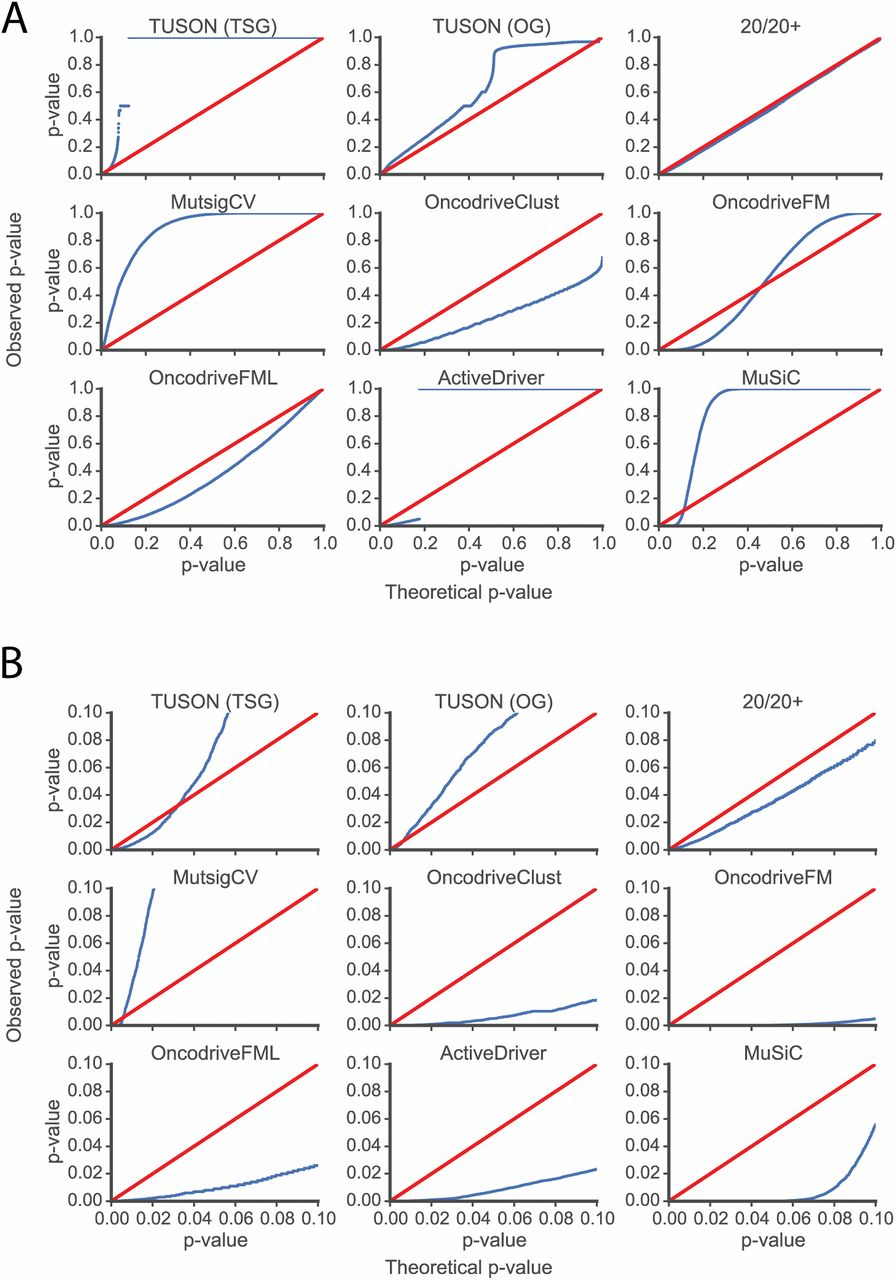
\includegraphics[width=0.9\linewidth]{figures/chapter4/qq_plots.jpg}
  \caption{Quantile-quantile plots comparing observed and theoretical P values for the tested methods. (A) Full P value range from 0 to 1. (B) Blowup of P values from 0 to 0.1. Observed P values for the methods (blue) are compared with those expected from a uniform distribution (red). Genes predicted as drivers by at least three methods were removed along with genes in the CGC. TUSON OG and TSG P values are shown separately.}
  \label{fig:qq_plot}
\end{figure}

\subsection{MLFC and mathematical justification}
\label{sec:mlfc_justification}

The MLFC is a metric of discrepancy between an observed P value distribution reported by a method and a theoretical uniform null distribution. I define MLFC as follows,

\begin{equation}
MLFC=1/n\sum_{i=1}^{n}{\left|\log_2{\frac{P(i)}{i/n}}\right|}
\end{equation}

where P(i) = i'th smallest P value, n is the total number of genes after excluding likely driver genes, and i/n is the corresponding expected P value from a uniform distribution. Values of MLFC near zero indicate smaller discrepancies, and therefore better statistical modeling of the passenger gene null distribution. The absolute value was included to prevent p-value distributions which show evidence of over-dispersion from effectively canceling out over-estimation of p-values with under-estimation in other p-values (see OncodriveFM, \autoref{fig:qq_plot}A).

All methods evaluated in the benchmark here used the Benjamini-Hochberg (BH) method \cite{RN94} to control the false discovery rate. The BH procedure rejects hypotheses by selecting the largest index g such that,

\begin{equation}
\frac{P(i)}{i/n} \leq q^*
\end{equation}
where $q^*$ is the desired false discovery rate control, and then rejecting all hypotheses $H(i)$ from index $i=1,..,g$. The critical part of the MLFC equation is the ratio of observed p-value to expected, which is intentionally the same statistic used in the Benjamini-Hochberg method. There are alternative approaches for testing whether a probability distribution differ from theoretical expectations, such as the Kolmogorov-Smirnov (KS) test \cite{RN100}. The KS test evaluates the significance of the maximum absolute differences between cumulative distribution functions. However, given the large number of hypothesis tests, even small absolute differences in the cumulative distribution at small p-values may result in many false positives. Moreover, I reasoned that in contrast to MLFC, the KS statistic does not directly relate to the BH procedure and disproportionately focuses on discrepancies at large p-values, which are of less practical interest.

\section{Number of Predicted Driver Genes}

The number of predicted driver genes ($q \leq 0.1$) ranged from 158 (MutsigCV) to 2,600 (OncodriveFM) (\autoref{fig:benchmark_result}C). There were two obvious categories of methods with respect to predicted driver genes: MutSigCV, 20/20+, and TUSON predicted 158-243 genes, whereas the remaining had over 400 driver genes.

\section{Driver Gene Prediction Consistency}

Statistical methods suffer from both systematic and random prediction errors. When no gold standard is available, it is difficult to estimate systematic error, but possible to estimate random error by measuring the variability of predictions. I tested the eight methods on 10 repetitions of a random two-way split of the all samples in our dataset, while maintaining the proportion of samples in each cancer type. An ideal method would produce the same list of driver genes, ranked by P value, for each half of the split. For a fair comparison, I considered that methods predicting many drivers would be less likely to have consistent rankings than those predicting only a few. Thus, I developed a measure named TopDrop consistency (TDC) (see \autoref{sec:tdc_limitations}) that examines the overlap between genes ranked at a defined depth (e.g., the top 100 genes) for each half of the random split. Examining TDC at a depth of 100 genes showed MuSiC, 20/20+, and TUSON to be the three with the highest consistency (\autoref{fig:benchmark_result}D). Most methods decreased in consistency when the gene depth was varied between 20 and 300, but the ordering of the TDC scores among the eight methods remained relatively stable.

\subsection{TopDrop consistency and limitations}
\label{sec:tdc_limitations}

Consistency assesses stability in gene ranking. Each method was applied to 10 repeated random splits, consisting of two disjoint halves of the full data. For pancancer assessment, the proportion of samples from each cancer type was maintained in each half. Disjoint halves were scored separately by each method, and genes were ranked from low to high P values. For a fair comparison between methods, I considered a specific depth of top-ranked genes, rather than a fixed q value threshold. This is because consistency becomes harder to achieve as the number of top-ranked genes gets larger. For example, a method that predicts 100 significant genes at $q \leq 0.1$ has an advantage in consistency over a method that predicts 1,000 significant genes at that threshold. I define $TopDrop consistency=|I_d |/d$, where $d$ is the designated depth of interest for the ranked gene list and $I_d$ is the TopDrop intersection, $I_d=A^{(1:d)} \cap B^{(1:2d)}$, defined as the intersection between predictions from the two random halves "A" and "B" such that the top d genes in "A" do not fall past twice the designated depth (2d) in "B."

I expect that all methods will lose statistical power and have greater random sampling error when they are predicting on a dataset that has been split in half. Therefore, I chose to allow genes to fall twice as far down the list in the "B" half of the split, to better distinguish random effects and methods with intrinsically low consistency.

A substantial limitation is TopDrop only evaluates consistency with independent identically distributed samples from the same data set. A better alternative would be to evaluate cross-study consistency \cite{RN157}, as there may be multiple reasons why findings in one study would not generalize to another. However, from a practical perspective, I can only use data currently available to evaluate performance.

\section{Overall Performance}

In \autoref{tab:overall_performance}, I summarize the performance of each method according to the criteria described above on the pancancer mutation data. The overall protocol is shown as a flowchart in \autoref{fig:flow_chart}. I assume that a preferable method would predict a higher fraction of driver genes that overlap with the CGC, that overlap with at least one other method, that have the least deviation from expected null P values, and that have the highest consistency. Each method is accordingly ranked by these four criteria and the average rank is shown. The top ranked methods are 20/20+, TUSON, OncodriveFML, and MutsigCV.

\begin{landscape}
\begin{tabular}{p{3cm} p{3cm} p{2cm} p{2cm} p{2cm} p{2cm} p{2cm}}
\toprule
  Method & No. significant genes &  CGC rank &  Consensus rank &  Pvalue rank &  Consistency rank &  Average rank \\
\midrule
  2020+ &  208 &  1 &  2 &  1 &  2 &  1.50 \\
  TUSON &  243 &  2 &  1 &  2 &  3 &  2.00 \\
  OncodriveFML &  679 &  4 &  4 &  3 &  4 &  3.75 \\
  MutsigCV &  158 &  3 &  3 &  4 &  6 &  4.00 \\
  OncodriveClust &  586 &  5 &  5 &  6 &  7 &  5.75 \\
  MuSiC &  1,975 &  7 &  8 &  8 &  1 &  6.00 \\
  ActiveDriver &  417 &  6 &  7 &  5 &  8 &  6.50 \\
  OncodriveFM &  2,600 &  8 &  6 &  7 &  5 &  6.50 \\ 
\bottomrule
\end{tabular}
\end{landscape}

\begin{figure}
  \centering
  \makeatletter
  \let\@currsize\normalsize
  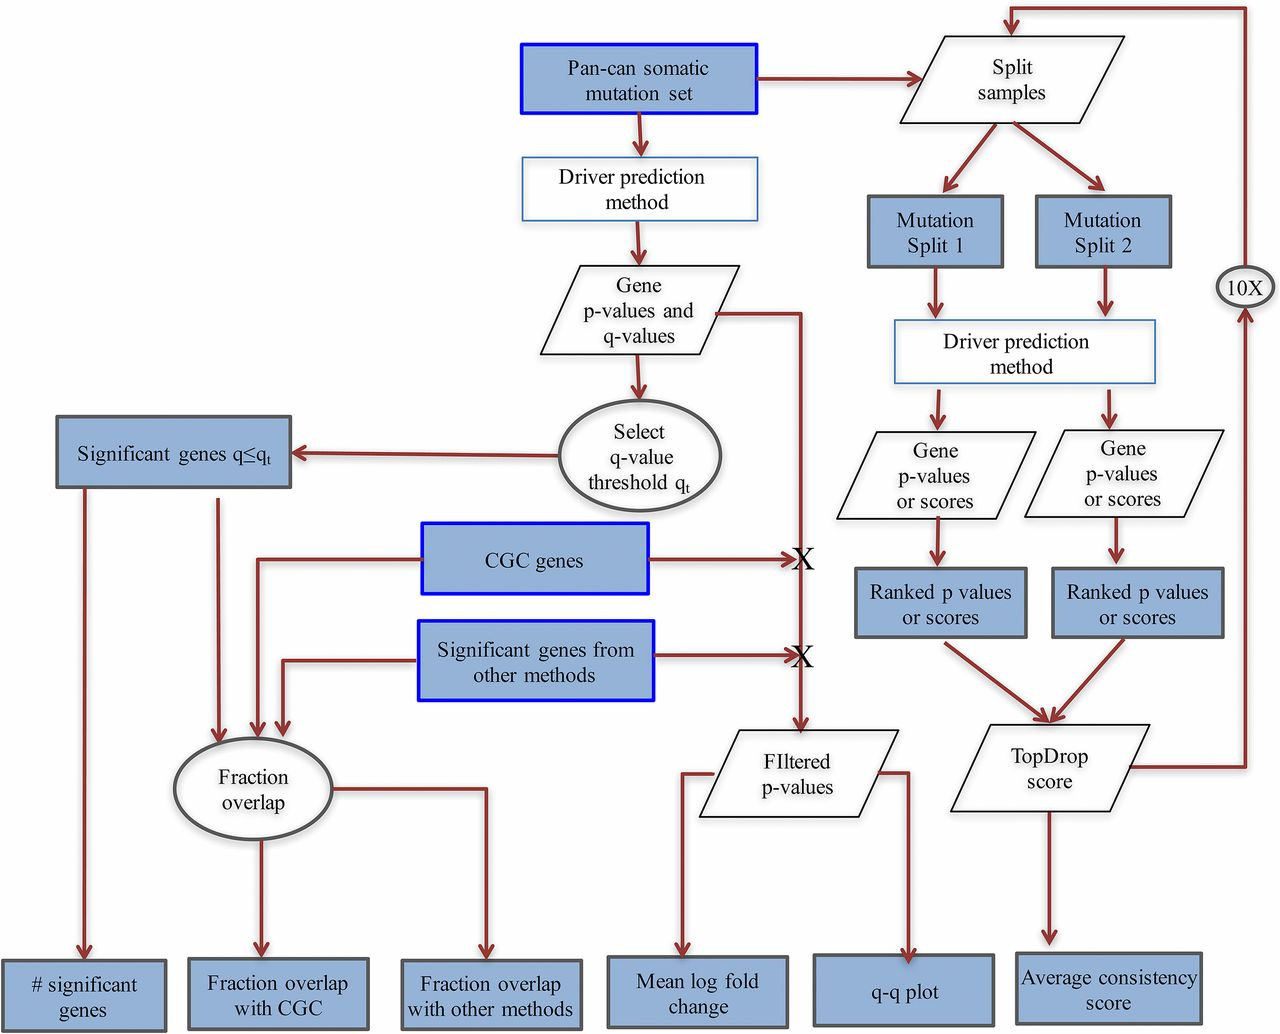
\includegraphics[width=0.9\linewidth]{figures/chapter4/flow_chart.jpg}
  \caption{Flowchart of evaluation protocol. Overview of how a driver gene prediction method of interest can be evaluated. The input to the method is the pancan somatic mutation set provided in this work \cite{RN70}. The initial output from the method to be evaluated is a list of predicted driver genes with associated P values and q values. A list of significant driver genes is produced by selecting a q value threshold. To compute fraction overlap of genes predicted as significant with Cancer Gene Census (CGC) and with the eight methods evaluated here, a freeze of CGC and predictions from the eight methods are provided. These gene lists are also used to subtract out putative driver genes and yield a list of filtered P values. Method consistency is estimated by 10 iterations of splitting the pancan somatic mutation set, outputting gene P values and scores for both halves, and applying the TopDrop metric. Jupyter notebooks for computing MLFC and qq plots from the filtered P value list, and the average TDC score are available at github.}
  \label{fig:flow_chart}
\end{figure}

\section{Conclusion}

A major goal of the huge public investment in large-scale cancer sequencing has been to find driver genes. Robust computational prediction of drivers from small numbers of somatic variants is critical to this mission, and it is essential that the best methods for this purpose be identified. Although many such methods have been proposed (see review \cite{RN49}), it has been difficult to evaluate them because there is no gold standard to use as a benchmark. Here, I developed an evaluation framework for driver gene prediction methods that does not require a gold standard. The framework includes a large set of small somatic mutations from a wide range of cancer types and five evaluation metrics. It can be used to systematically evaluate new prediction methods and compare them to existing methods. The results would be more informative to users of these methods than current ad hoc approaches.

To apply the framework to a new method (\autoref{fig:flow_chart}), a ranked list of predicted driver genes can be generated from the pancancer mutation dataset, including a P value and a Benjamini-Hochberg corrected q value for each gene. The choice of a threshold $q \leq 0.1$ to define driver genes worked well in our evaluations but can be adjusted if so desired. The same threshold should be used for fair comparison of different methods. If a driver prediction tool does not produce P values, a raw score threshold that represents the desired false-discovery rate could be selected.

The MLFC also has substantial implications for the accuracy of driver gene prediction methods. The relatively high MLFC of several methods brings into question the validity of the assumptions or analytic methods used in their construction. I believe that the most likely problem is with the assumptions rather than the analytic methods, which all appear to be well thought-out. In addition, the most likely problem with the assumptions is that there is unexplained variability in the background mutation rates (see \autoref{chap:ch2}). This variability may be tumor type specific or even patient or tumor specific. If P values are underestimated in the range of low p-values, too many genes will be called as drivers. In fact, the methods that underestimate P values predict the largest number of drivers and have the highest fraction of uniquely predicted drivers.



%!TEX root = root.tex

\chapter{HotMAPS: Exome-scale discovery of mutation hotspots in 3D protein structure}
\label{chap:ch5}
\chaptermark{HotMAPS}

\section{Introduction}

Missense mutations are perhaps the most difficult mutation type to interpret in human cancers. Truncating loss-of-function mutations and structural rearrangements generate major changes in the protein product of a gene, but a single missense mutation yields only a small change in protein chemistry. The impact of missense mutation on protein function, cellular behavior, cancer etiology, and progression may be negligible or profound, for reasons that are not yet well understood. 

Recurrence of missense mutations in cancers at the same amino acid residue position is well known to be a characteristic feature of both oncogenes (OG) and tumor suppressor genes (TSG; \cite{RN107}). The observation that somatic mutations also frequently occur in positions proximal in protein sequence to the most highly recurrent positions has suggested that positional clustering of somatic missense mutations might be used to identify drivers \cite{RN109}. These clusters, known as \q{hotspots,} are regions where somatic missense mutations occur closer together in protein sequence than would be expected by chance. Hotspot regions can be rationalized as areas in a protein under positive selection in the cancer environment; missense mutations occurring in these regions are selected for because they alter protein function in a manner advantageous to the cancer cell. Numerous methods have been developed to identify hotspots based on the linear protein sequence \cite{RN16, RN46, RN110, RN87, RN54, RN55}.

Only using the linear sequence of a protein, however, may fail to capture hotspots that appear in the 3-dimensional (3D) structure of a protein \cite{RN105}. Protein structure has long been known to relate to the function of a protein \cite{RN112, RN113}, and clustering of mutations within a structure may indicate mutations that are cancer drivers. An algorithm that leverages 3D protein structure information, but still performs clustering in 1D through a dimensionality reduction step, has shown utility in detecting oncogenes \cite{RN15}. A recent study of an aggregated collection of TCGA cancer mutations from 21 tumor types presented an algorithm to identify cancer genes based on 3D clustering of somatic missense mutations, yielding ten such genes \cite{RN105}. 

Here, I present HotMAPS (Hotspot Missense mutation Areas in Protein Structure), a new, sensitive algorithm for high-throughput analysis of cancer 3D hotspot regions of missense mutation. HotMAPS finds clusters of amino acid residues with significantly increased local mutation density in 3D protein space, compared with an empirical null distribution. The statistical model is designed to handle higher-order protein complexes and can capture regions that span protein-protein interfaces. I apply HotMAPS to missense mutations from 23 tumor types sequenced by TCGA. By careful use of both experimentally derived protein biologic assemblies in the Protein Data Bank (PDB) and theoretical protein structure models, I substantially increase the number of amino acids that can be mapped into 3D protein space and the number of detectable hotspot regions compared to a prior approach \cite{RN105}.

\section{HotMAPS algorithm}

Standard clustering algorithms are not well suited for detecting rare clustering patterns in a large number of problems. I considered many standard clustering algorithms for clustering mutations in protein structure \cite{RN117, RN114, RN115, RN116}, but each has substantial weaknesses. Methods like K-means and spectral clustering require the number of clusters to be specified as a parameter, but the number of clusters is not necessarily the same for every protein structure. In practice, the \q{elbow-method} is used where the number of clusters is chosen manually by examining where there is a noticeable flattening in performance as the number of clusters is increased \cite{RN118}. However, when applying clustering to ~65,000 protein structures, manual procedures are infeasible. Even if the clustering algorithm doesn't need the number of clusters as a parameter, such as affinity propagation \cite{RN114} or DBSCAN \cite{RN117}, they generally assume the minimum number of clusters is one. Since driver mutations are rare relative to all mutations, most protein structures should have no clusters due to the clustering of driver mutations.

There are also application specific concerns for clustering mutations in protein structure. A clustering algorithm would preferably adjust for the topology of a protein structure as this affects where mutations could possibly be located. Additionally, since protein structure may contain multiple identical protein subunits, a clustering algorithm needs to compensate for the non-independence of mutations. Lastly, the algorithm should ideally statistically adjust for potential false discovery of clusters due to the large number of clustering problems (~65,000 protein structures). 

The HotMAPS algorithm was developed to address all of these noted limitations and is described below (\autoref{fig:hotmaps_algorithm}).

\begin{figure}
  \centering
  \makeatletter
  \let\@currsize\normalsize
  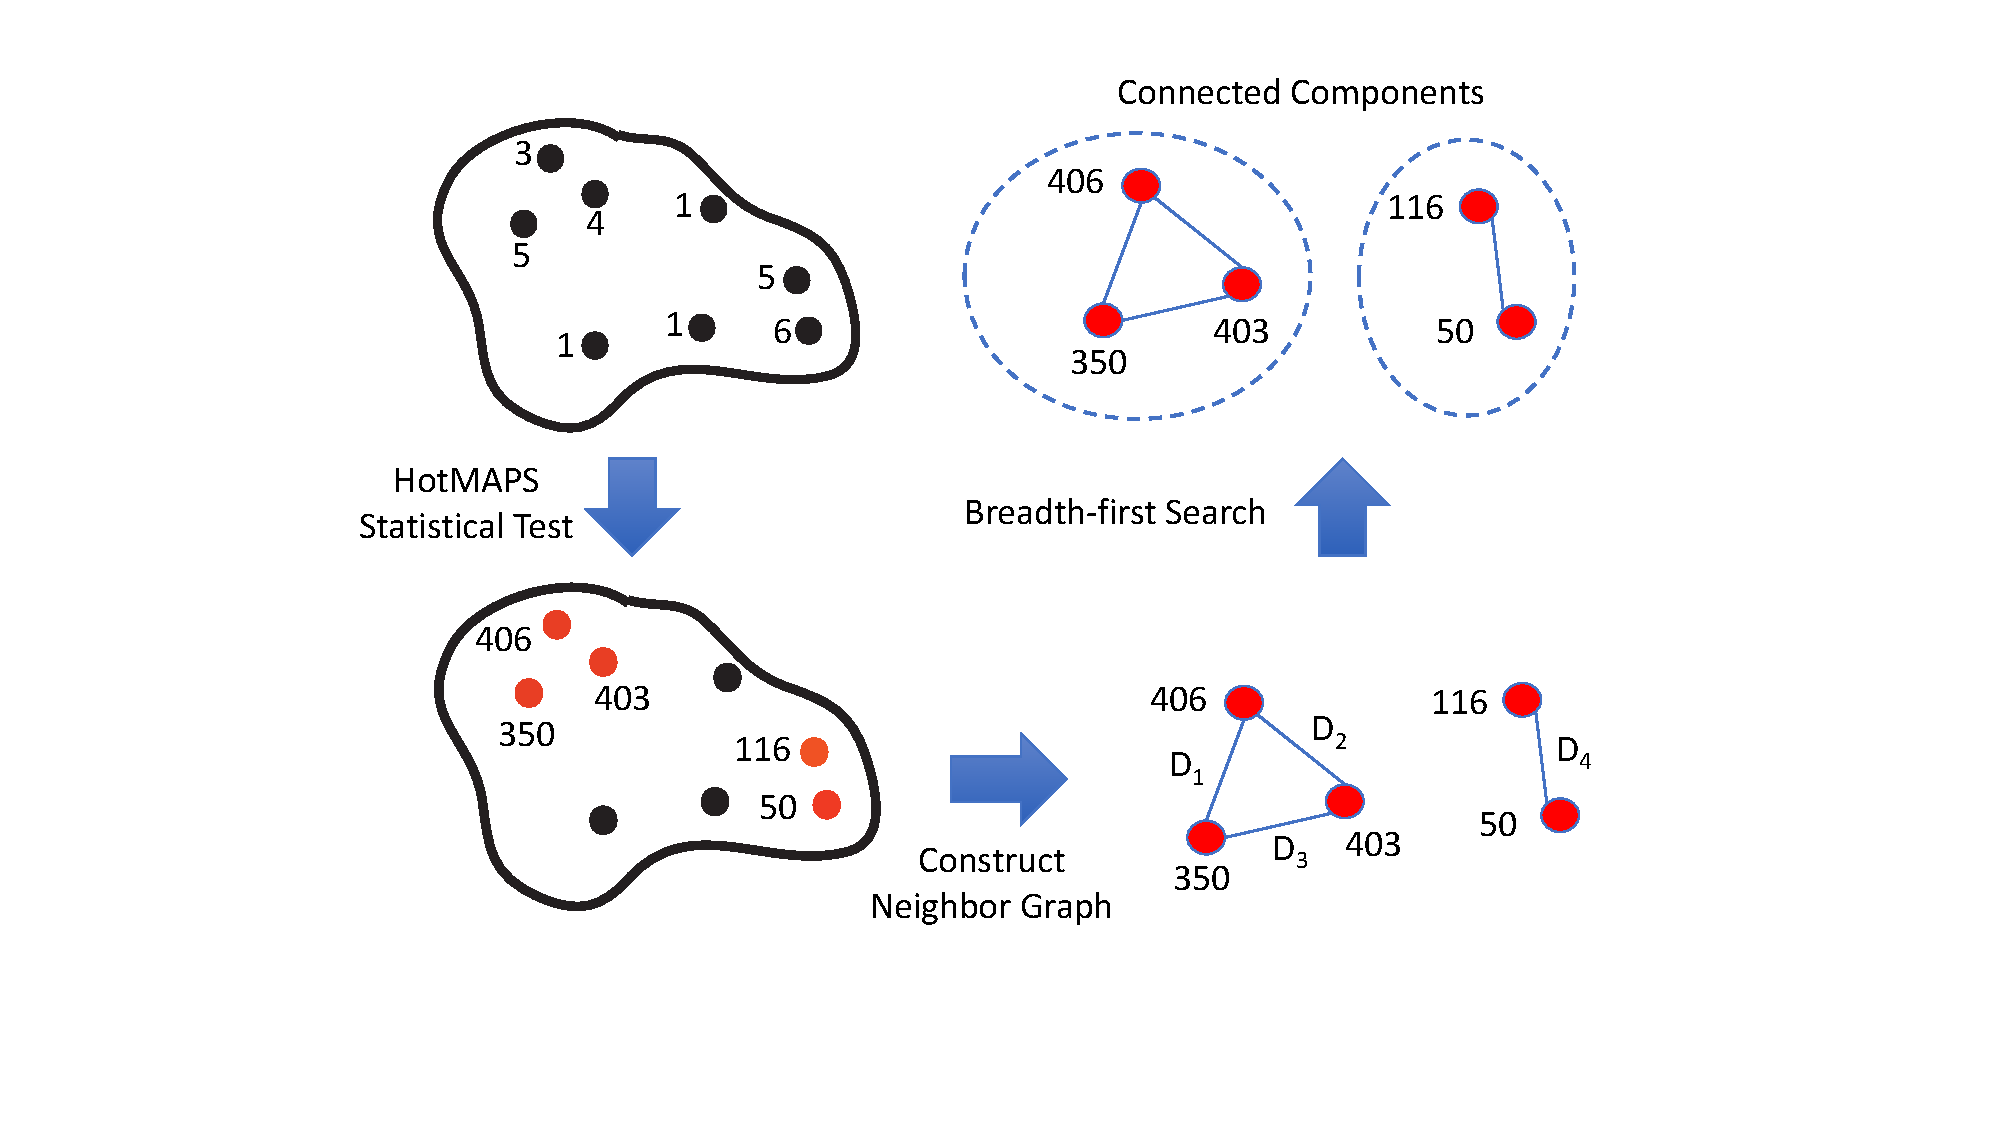
\includegraphics[width=0.9\linewidth]{figures/chapter5/hotmaps_algorithm.pdf}
  \caption[Algorithmic flowchart for Hotspot Missense mutation Areas in Protein Structure (HotMAPS) algorithm.]{HotMAPS was run on 65,372 protein structures and models.  For each structure or model, mutations were mapped from TCGA genomic coordinates to 3D protein space and for each mutated residue, its observed local mutation density was calculated. P-values were estimated based on simulations. If p-values for the same residue differed across multiple structures/models, the minimum was used and adjusted for multiple hypotheses testing with the Benjamini-Hochberg algorithm.  Hotspot regions were identified as connected components in a graph of significantly mutated residues.}
  \label{fig:hotmaps_algorithm}
\end{figure}

\subsection{Mutation density}

HotMAPS depends on calculating a mutation density for each amino acid residue. Let K be the set of all protein structures.  Each protein structure or model was an element $k\in K$.  For each k, the center of geometry in Euclidean space (i.e., centroid) was calculated for each residue ($r$), considering all backbone and side-chain atoms,

\begin{equation}
C_r^k = \frac{1}{|r|}\sum_{a\in r}{a}
\end{equation}

where $C_r^k$ is the center of geometry for residue $r$ in $k$, and a is a 3D position vector for each atom in residue $r$. The neighbors of residue $r$ were identified using a 10 angstrom radius cutoff from the center of geometry,

\begin{equation}
N_r^k = \{r' : dist(C_r^k, C_{r'}^k) \leq 10, r' \in R^k \}
\end{equation}

where $R^k$ is the set of residues for $k$, $N_r^k$ is the set of neighbor residues for residue $r$, and $dist$ is the Euclidean distance function. The density D of mutations at residue $r$ was calculated as the sum of mutations in the residue's neighborhood,

\begin{equation}
D_r^k = \sum_{n \in N_r^k}{M^k_n}
\end{equation}
\begin{equation}
D^k_{obs} = \{D^k_r : M^k_r>0, r \in R^k\}
\end{equation}

where $M_n^k$ is the number of missense mutations for the n'th residue neighbor, $D_r^k$ is the density of mutations for a specific residue and $k$, and $D_{obs}^k$ is the set of observed mutation densities for all mutated residues in a given $k$.

\subsection{Statistical model}

Next, I simulated a null distribution expected if mutations on the protein structure were under no selective pressure to occur in any particular region.   The null distribution is reasonably modeled by a discrete uniform distribution. Mutations occurring under the null were simulated by sampling with replacement a number of residues equal to the total observed mutations,

\begin{equation}
M_{sim}^k \sim Uniform(R^k, Size=\sum{M_r^k})
\end{equation}

where $M_{sim}^k$ is the simulated missense counts for all residues in $k$.  The procedure was modified slightly for protein complexes, containing multiple protein chains that originated from a single gene product (e.g., a homodimer). I accounted for this non-independence by running identical simulations simultaneously on multiple duplicated protein chains.  Duplicate chains were identified based on either having same PDB chain letter and/or the same chain description. The mutation density for simulated mutations was calculated in the same manner as the observed mutations. The procedure was repeated for 10,000 iterations on each structure.

Based on the empirical null distribution established from simulations, I calculated the one-tailed p-value for each residue's mutation density being equal or larger,

\begin{equation}
P^k_r = \frac{\#\{d : d \geq D^k_r, d \in D^k_{sim}\}}{\#\{d \in D^k_{sim}\}}
\end{equation}

where $D_{sim}^k$ is the set of all simulated mutation densities and $P_r^k$ is the p-value for residue $r$ in $k$. Since there may be many structures and/or models that cover the same corresponding portion of the genome, multiple p-values were collapsed by taking the minimum p-value among residues that mapped to the same genomic codon. These unique genomic-level p-values were then corrected for multiple hypotheses by the Benjamini-Hochberg method \cite{RN94} and deemed significant at a q-value of 0.01. I selected the very conservative q=0.01 empirically, to minimize the number of false discoveries in our study.  Identifying the corresponding significant residues at the structure (or model) level was backtracked by using the supremum of significant p-values at the codon level as a cutoff,

\begin{equation}
P^* = \sup{\{P_c : q_c < 0.01, \forall c\}}
\end{equation}
\begin{equation}
R^k_{signif} = \{r : P^k_r \leq P^*, \forall r\}
\end{equation}

where $P_c$ and $q_c$ are the genomic p-value and q-value, respectively, for codon $c$, $P^*$ is the p-value cutoff adjusted for multiple hypotheses, $R_{signif}^k$ is the set of significant residues for $k$.

\subsection{Constructing hotspot regions}

3D mutation hotspot regions were identified as groupings of significant residues, according to the principle of maximum parsimony.  Specifically, I found the minimum number of non-contiguous hotspot regions that explained all significant residues. I first constructed a neighbor graph amongst significant residue positions, where edges were created if two residues could be considered as neighbors, defined as within 10 angstroms (1nm), which is the order of magnitude for the length of an amino acid residue side chain. 3D mutation hotspot regions for each k were then found as the connected components of the neighbor graph using breadth-first search. Our results were not very sensitive to small perturbations of this parameter (8\AA, 9\AA, 11\AA, 12\AA). The 10\AA maximum distance identified 85\% of the hotspot residues identified at the four other threshold values.

\section{Mapping mutations to protein structure}

\subsection{Mutational data set}

Mutation annotation format (MAF) file data for 23 tumor types from The Cancer Genome Atlas (TCGA) was downloaded by the Xena data store (\url{https://genome-cancer.soe.ucsc.edu/proj/site/xena/hub/}) using their API.

\subsection{Protein structure}

PDB structures were obtained from the Worldwide Protein Data Bank (PDB) (10/17/2015). Only structures solved by x-ray crystallography and containing at least one human protein chain were used.  To avoid computation on crystal-packing artifacts that are common in PDB multi-domain protein structures and proteins in complex with other proteins or DNA/RNA structures, I used PDB biological assemblies that model how proteins exist in vivo (\url{ftp://ftp.wwpdb.org/pub/pdb/data/biounit}). Additionally, single-domain, theoretical protein structure models constructed based on homology to non-human proteins were included to increase coverage over a greater proportion of genes. Theoretical models were obtained from the ModPipe human 2013 dataset (\url{ftp://salilab.org/databases/modbase/projects/genomes/H_sapiens/2013/}), built with Modeller 9.11 \cite{RN119}.   In addition to criteria required by ModPipe (ModPipe Protein Quality Score $>$ 1.1), theoretical models were further filtered to increase the quality of structures used in our assessment, requiring that: 1) models had a minimum length of 75 residues. 2) The sequence of the target human protein and the sequence of the non-human homolog used for homology modeling were $\geq$10\% identical. 3) The \q{loop} content of the protein model was $\leq$30\%. 4) Compactness score $C$ (see \autoref{eq:compactness}) was $\leq$1\AA/residue. The compactness score was based on the protein radius of gyration ($R_g$), and was employed to reject overly extended or unfolded structures. All thresholds were selected by visual inspection of structures meeting each of the four criteria.

Theoretical protein structure compactness score filter:
\begin{equation}
\label{eq:compactness}
C = \frac{4R_g}{N}
\end{equation}
\begin{equation}
\text{where } R_g=\sqrt{\frac{\sum_i{m_i(\vec{r}_i-\vec{r}_c)^2}}{\sum_i{m_i}}} 
\end{equation}

where N is total number of residues. $m_i$ is the mass of the i'th atom, $\vec{r}_i$ is the center of the i'th atom, and $\vec{r}_c$ is the protein center of geometry.

\subsection{Mapping algorithm}

Mapping of genome coordinates was done using a modified version of the TransMap algorithm (\autoref{fig:mapping_algorithm}), previously described in \cite{RN120}. In a minority of cases mutations did not have a one-to-one mapping within a protein structure (0.6\% of mutations analyzed in this study were impacted). Any hotspot region residue positions with ambiguous mappings were dropped from the final analysis. Protein sequences in the UniProt database (SwissProt curated only) \cite{RN121} were aligned to all transcripts in RefSeq, CCDS and Ensembl databases with tBLASTn \cite{RN122}.  Transcripts were then aligned to human genome assembly GRCh37 (hg19) with BLAT \cite{RN123}.  BLAT was also used to align the UniProt protein sequences with PDB SEQRES amino acid residue sequences (\autoref{fig:mapping_algorithm}).  For theoretical models, ModPipe provided a RefSeq or Ensembl transcript identifier and translation of each transcript into protein sequence, eliminating the need for the tBLASTn step to align protein sequence to transcript. 

\begin{figure}
  \centering
  \makeatletter
  \let\@currsize\normalsize
  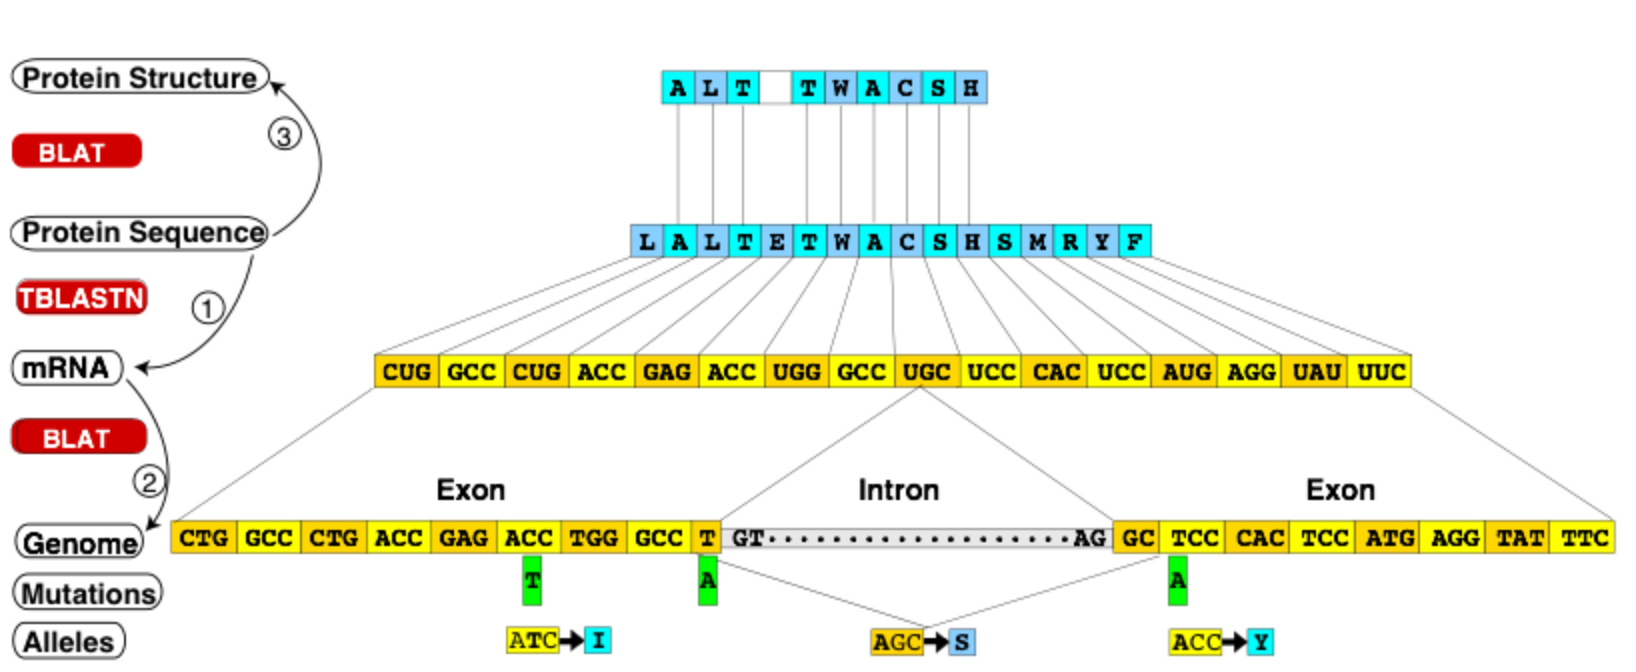
\includegraphics[width=0.9\linewidth]{figures/chapter5/mapping_algorithm.png}
  \caption[Mapping of genomic coordinates onto protein structures and models with a modified version of the TransMap algorithm.]{The mapping is done with three pairwise alignment steps, using tBLASTn and BLAT.  Projection of protein sequence coordinates to mRNA transcript coordinates (1) and finally genomic coordinates (2) is done \q{top down}. The process enables handling of split codons, such as the \q{AGC} shown.  Protein sequence coordinates are subsequently projected into the PDB coordinate system of protein structure (3).}
  \label{fig:mapping_algorithm}
\end{figure}

\section{3D mutation hotspot regions are important in cancer}

\subsection{3D hotspot regions are enriched in well-known cancer genes}

Among the set of genes with available protein structure or models (n = 15,697), the genes harboring a 3D hotspot region are enriched for OGs and TSGs (P = 6.1E−30 for OGs and P = 2.4E−13 for TSGs; one-tailed Fisher exact test). They are also enriched for genes in the CGC list (P = 1.4E−30; one-tailed Fisher exact test). The subset of these genes harboring only a 3D hotspot region not detectable in 1D is also significantly enriched (P = 4.3E−09 for OGs, P = 7.9E−12 for TSGs, P = 8.0E−11 for CGC genes; one-tailed Fisher exact test). An additional 23 genes that are proposed OGs, TSGs, and/or drug targets or hereditary cancer genes contained at least one 3D hotspot region. This enrichment of known and candidate driver genes supports my claim that many of the regions are biologically relevant and not simply artifacts. While regions were detected in only approximately 18\% of established cancer genes, I expect that many of these genes harbor drivers other than missense mutations, some are drivers in tumor types not represented in our study and many lack structural coverage.

\subsection{Mutations in 3D hotspot regions are different from other somatic mutations in cancers}

I examined whether the amino acid residue positions and the missense mutations in the 3D hotspot regions had distinctive features suggestive of a special biologic importance, when compared with the remaining mutations in our study. Four candidate distinguishing features were tested: (i) vertebrate evolutionary conservation; (ii) occurrence at a protein-protein interface, which increases the potential for a missense mutation to disrupt protein-protein interactions; (iii) in silico cancer driver scores generated with the CHASM algorithm \cite{RN29}; and (iv) in silico pathogenicity scores generated with the VEST algorithm \cite{RN30}, which are predictors of increased missense mutation impact (\autoref{fig:hotspot_properties}). In comparison with mutated residues not in 3D hotspot regions, vertebrate evolutionary conservation was higher and protein-protein interface occurrence was higher in the 3D hotspot regions (conservation P = 2.9E−29, Mann-Whitney U test; protein interface P = 5.2E−13, one-tailed Fisher exact test). In silico driver scores and pathogenicity scores were higher for missense mutations in 3D hotspot regions (driver score P = 3.0E−47, pathogenicity score P = 3.0E−16; Mann-Whitney U-test) than for the remaining mutations (\autoref{fig:hotspot_properties}).

\begin{figure}
  \centering
  \makeatletter
  \let\@currsize\normalsize
  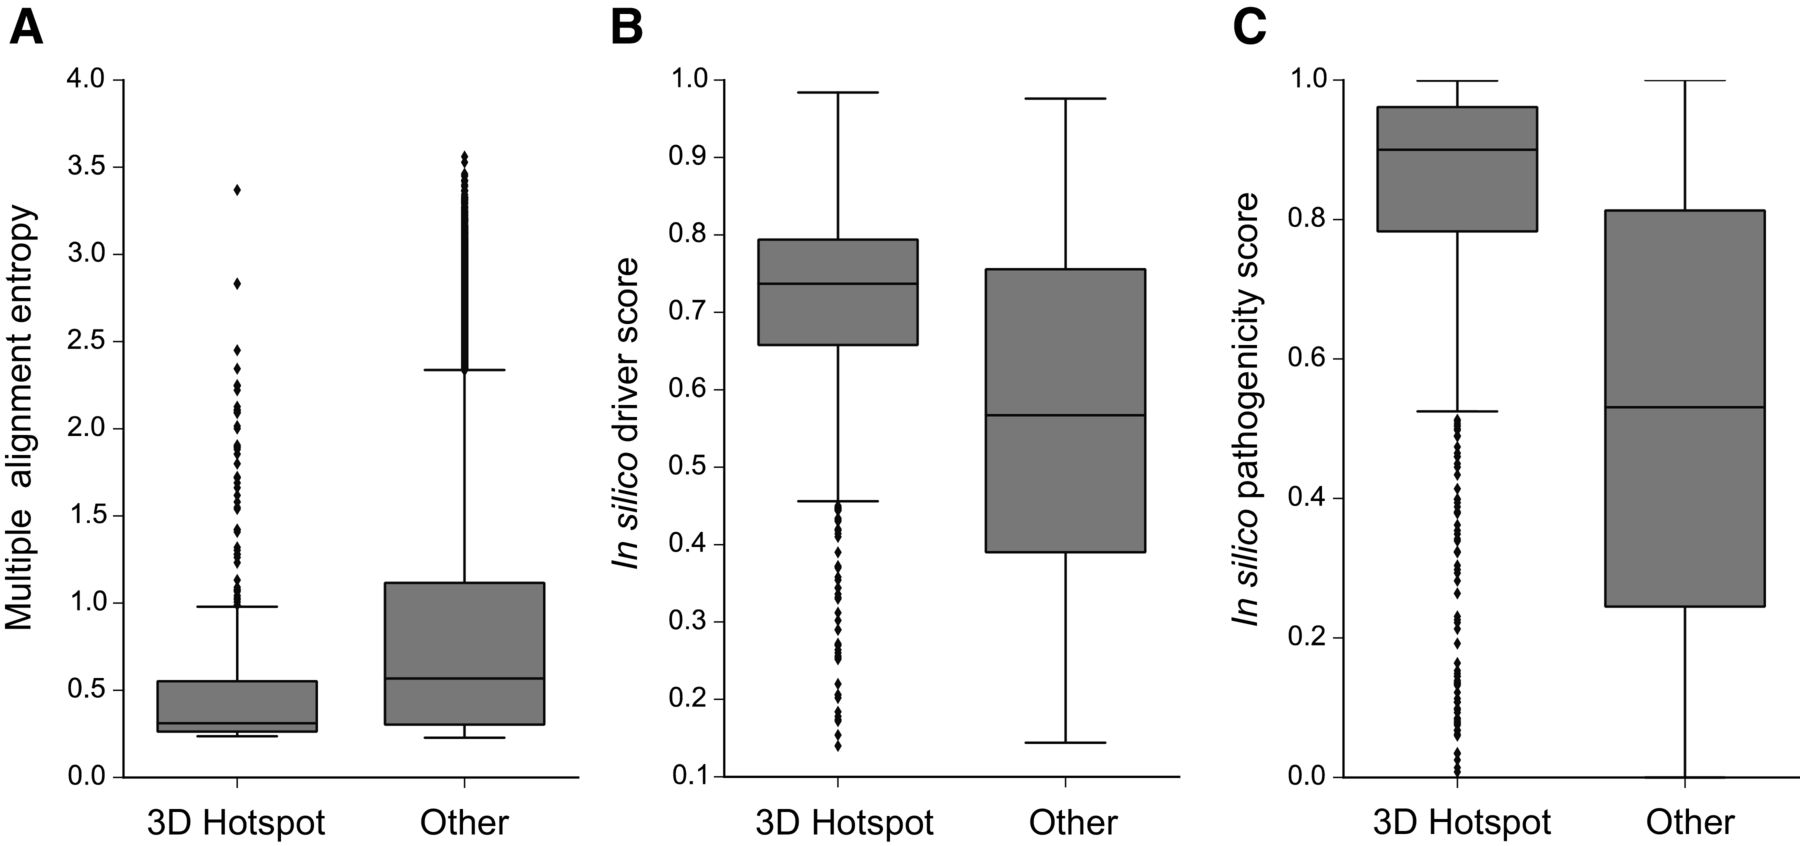
\includegraphics[width=0.9\linewidth]{figures/chapter5/hotspot_properties.jpg}
  \caption[3D hotspot regions are different from other mutated protein residues.]{Three distinguishing features of HotMAPS regions. A, HotMAPS-mutated residues are more conserved in vertebrate evolution than mutated residues not in hotspot regions, as shown by lower multiple alignment entropy (P = 1.2E−29; Mann-Whitney U test). Multiple alignment entropy is calculated as the Shannon entropy of protein-translated 46-way vertebrate genome alignments from UCSC Genome Browser, which is lowest for the most conserved residues. B and C, HotMAPS missense mutations have higher in silico cancer driver scores from the CHASM algorithm (P = 5.3E−47; Mann-Whitney U test) than those mutations not in hotspot regions (B) and higher in silico pathogenicity scores from the VEST algorithm (P = 7.0E−162; Mann-Whitney U test; C). Finally, HotMAPS-mutated residues occur more frequently at protein-protein interfaces (P = 1.3E−11; one-tailed Fisher exact test).}
  \label{fig:hotspot_properties}
\end{figure}

\subsection{3D hotspot regions are different in oncogenes and tumor suppressor genes}

The catalog contains 37 regions stratified by tumor type in bonafide tumor suppressor genes and 77 in bonafide oncogenes (114 regions in 30 genes), using as a benchmark the classifications of Vogelstein and colleagues (landscapes benchmark; \cite{RN25}). I used these data to explore possible differences between tumor suppressor gene and oncogene regions at amino acid resolution. I found that in tumor suppressor genes, 3D hotspot regions were larger than in oncogenes (region size P = 9.6E−06; Mann-Whitney U test). They were also more mutationally diverse (mutational diversity P = 2.1E−07; Mann-Whitney U test). In addition, oncogene 3D hotspot regions were more conserved in vertebrate evolution and more solvent accessible in protein structure, meaning that they tend to occur at the protein surface (evolution P = 4.7E−07, solvent accessible P = 1.5E−06; Mann-Whitney U test). Hotspot regions in tumor suppressor genes harbored increased net change in hydrophobicity (P = 3.3E−07; Mann-Whitney U test) and net change in volume (P = 2.2E−07; Mann-Whitney U test), suggesting that their impact on protein function could be due to decreased stability. The in silico missense mutation cancer driver scores were higher for oncogene regions (P = 0.003; Mann-Whitney U test). I also tested differences between in silico pathogenicity scores and occurrence at protein-protein interfaces between OG and TSG regions, but these were not significant (pathogenicity scores P = 0.37, protein interface P = 0.34; Mann-Whitney U test).

The fact that these differences between oncogene and tumor suppressor gene regions were statistically significant suggested that they might have predictive value. Principal components analysis (PCA) of the six significant features indicated some separation (\autoref{fig:hotmaps_pca}A). Next, I trained a Naive Bayes machine learning classifier to discriminate between oncogene and tumor suppressor gene hotspot regions, using region size, mutational diversity, vertebrate conservation, residue solvent accessibility, mutation net hydrophobicity change, and residue volume change as features. A rigorous gene-level holdout protocol was used to avoid overfitting. A Naive Bayes score closer to 1.0 indicates that the hotspot region is likely in an OG while a score closer to 0.0 indicates that it is in a TSG. Area under receiver operating characteristic (ROC) curve or AUC, a standard measure of classifier performance, was 0.84 out of 1.0, a result that supports my claim that 3D hotspot regions in oncogenes and tumor suppressor genes have distinctive characteristics (\autoref{fig:hotmaps_pca}B). AUC of a classifier with random performance is 0.5. Performance did not improve when the other features were included in the classifier. The ROC performance and PCA plot support my claim that characteristic differences between oncogenes and tumor suppressor genes hotspots can be quantified. 

\begin{figure}
  \centering
  \makeatletter
  \let\@currsize\normalsize
  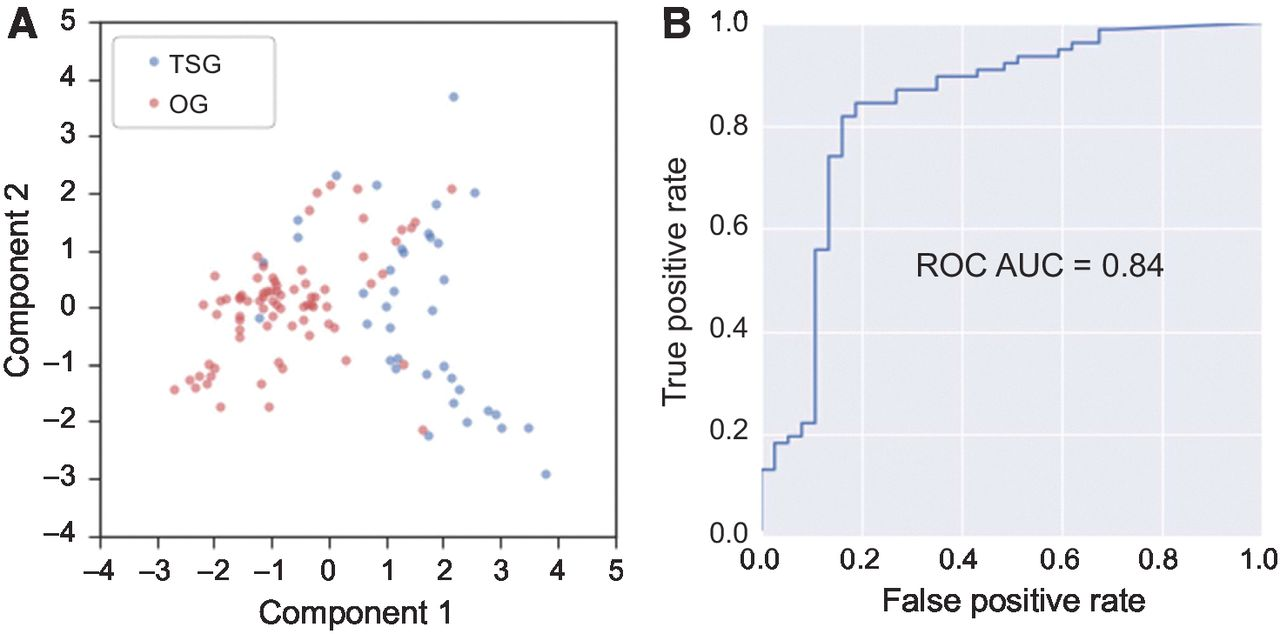
\includegraphics[width=0.9\linewidth]{figures/chapter5/pca.jpg}
  \caption[HotMAPS regions have different characteristic features in OGs and TSGs.]{A, PCA plot shows a clustering pattern in hotspot regions identified in oncogenes (OG=red) and tumor suppressor genes (TSG=blue). Each point is a region represented by six numeric features, projected into two dimensions. The features are region size, mutational diversity, vertebrate evolutionary conservation, residue relative solvent accessibility, mutation net change in hydrophobicity, and mutation net change in residue volume. B, OG and TSG HotMAPS regions can be discriminated with machine learning, based on six features. A Gaussian Naive Bayes classifier trained with the landscapes benchmark provides a reasonable separation between the two classes with AUC = 0.84 out of 1.0. Performance of a random classifier is AUC = 0.5. ROC, receiver operating characteristic; AUC, area under the ROC curve.}
  \label{fig:hotmaps_pca}
\end{figure}

\subsection{What is gained by 3D hotspot region detection versus 1D?}

The larger size and mutational diversity of hotspot regions in tumor suppressor genes (TSGs) versus oncogenes (OGs) suggest that they could be more difficult to detect and perhaps they have been underreported by 1D approaches. OG hotspot regions consisting of recurrent missense mutations at one or two residues can be seen by eye with lollipop plots and are straightforward to detect computationally based on 1D primary sequence. I hypothesized that detection of many TSG hotspot regions might require a 3D algorithm. To maximize the interpretability of this analysis, regions that occurred in multiple tumor types were merged so that each region was represented only once in each gene.

For a well-controlled comparison of 3D and 1D hotspot region detection, I applied a 1D version of our method to the protein chain sequences of the same set of PDB protein bioassemblies and theoretical protein structure models to detect nonuniform clustering patterns on primary protein sequence. Seventy-two percent of hotspot regions identified in 3D were identifiable in 1D.

Next, I compared the number of hotspot regions identified in OGs and TSGs. I considered regions identified in 3D only, in both 3D and 1D, and in 1D only. Using the bona fide OGs and TSGs (Table 1), there were significantly more OG regions that TSG regions identified by the 1D algorithm (P = 0.03; one-sided Fisher exact test). The 1D-only version of the algorithm detected 5 OG and 2 TSG regions; 1D further detected an additional 25 OG and 7 TSG regions that were also identified by the 3D algorithm. The 3D algorithm identified an additional 4 OG and 6 TSG regions. To increase our power, I repeated this test again using the bona fide OGs and TSGs plus additional regions in five candidate OGs and TSGs reported in the literature (OGs were FSIP2, MTOR, RANBP2, CHEK2, and MAPK1; TSGs were RASA1, SMARCA2, KEAP1, CUL1, TGFBR2; all are listed and cited in Table 2), yielding increased statistical significance (P = 0.009, one-sided Fisher exact test). The results suggest that 1D detection methods may be better suited to detecting regions in OGs rather than TSGs.

A further problem with sequence-based 1D hotspot region detection is that larger regions detectable in 3D may be only partially characterized and/or split into multiple pieces. \autoref{fig:benefits_3d_space} shows an example of a TSG hotspot region in FBXW7 found in 3D by HotMAPS that has been split into two pieces by the 1D algorithm. In 1D protein sequence, residue 465 is not close enough to residues 502 and 505 to be identified in one hotspot region. On the 3D protein structure of FBXW7 (PDB code 2OVQ), the three residues are spatially close and a single hotspot region is detected.

\begin{figure}
  \centering
  \makeatletter
  \let\@currsize\normalsize
  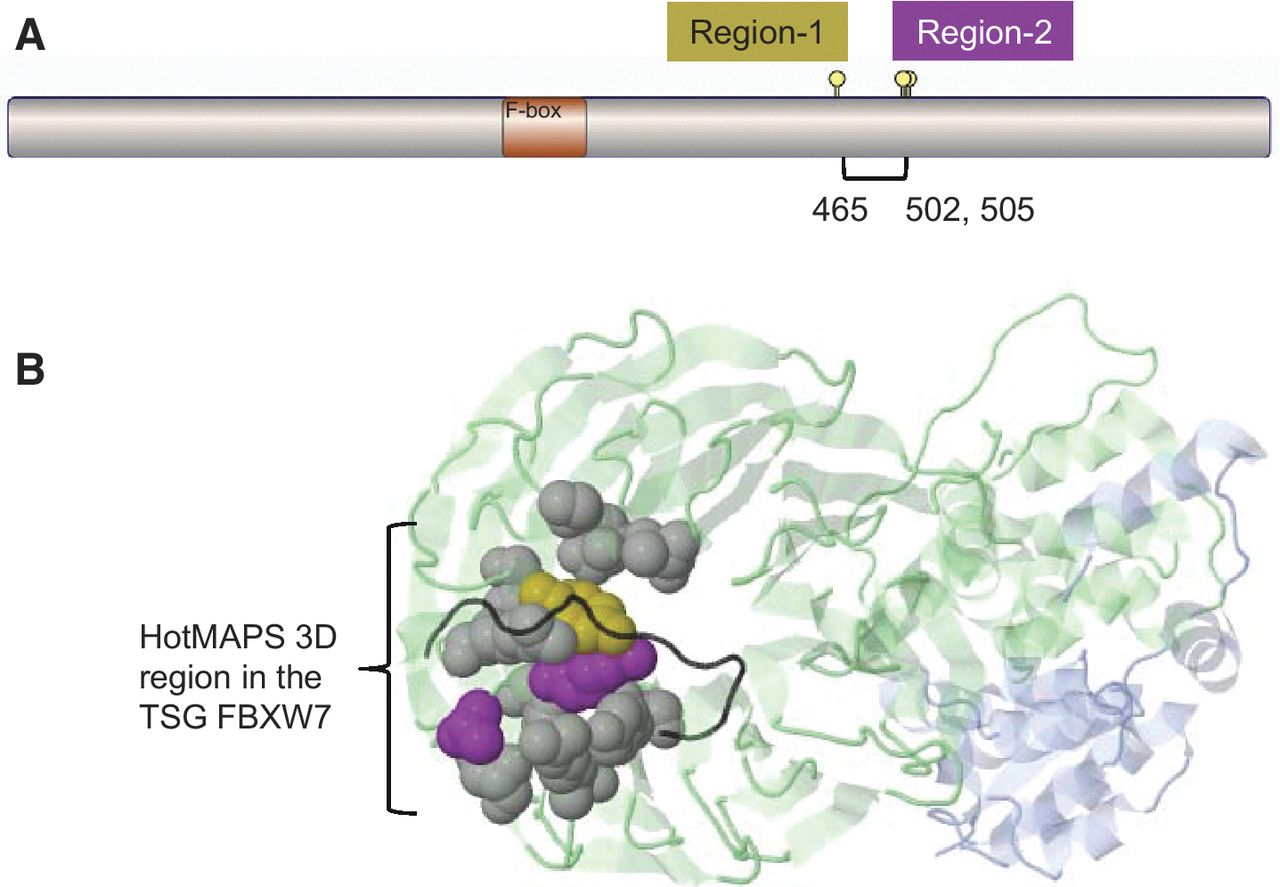
\includegraphics[width=0.9\linewidth]{figures/chapter5/benefits_3d_space.jpg}
  \caption[Comparison of hotspot detection in the TSG FBXW7 in 1D and 3D.]{Comparison of hotspot detection in the TSG FBXW7 in 1D and 3D. A, a simplified 1D version of HotMAPS found two regions in FBXW7. The 3D version of HotMAPS found a single larger region, encompassing both regions. Diagram shows protein sequence of FBXW7, which contains a single F-box functional domain. Region-1, residue 465 (left lollipop); Region-2, residues 502 and 505 (right lollipops). B, HotMAPS identifies a single 3D hotspot region in FBXW7. Structure of SCFFbw7 ubiquitin ligase complex (PDB 2OVQ), containing FBXW7 (green), SKP1 (blue), and CCNE1 fragment (degron peptide; black). Residue coloring: 1D Region-1, gold; 1D Region-2, purple. Residues missed by 1D detection but included in HotMAPS 3D, gray. Although the 1D regions are far in the primary protein sequence, residues 505 and 465 spatially contact at the interface with CCNE1. Protein structure figures were generated by JSMol in MuPIT (\url{http://mupit.icm.jhu.edu/}).}
  \label{fig:benefits_3d_space}
\end{figure}

\section{3D hotspot regions may increase interpretability of driver mechanisms}

Three-dimensional consideration of hotspot regions in protein structure can potentially provide researchers with a rich source of hypothesis generation about driver mechanisms. While gene- or domain-level mutation enrichment analysis can point to potential protein functions, interactions, biologic processes, and pathways important for cancer etiology and progression, more detailed information may be available once a specific set of mutated amino acid residues has been identified as significant.

For many of the 3D hotspot regions found by HotMAPS, the literature contains evidence that they are in direct contact with or proximal to amino acid residues of known functional importance. \autoref{fig:hotmaps_examples} shows six cancer-associated proteins in which the hotspot region is either overlapping or proximal to important functional sites.

\begin{figure}
  \centering
  \makeatletter
  \let\@currsize\normalsize
  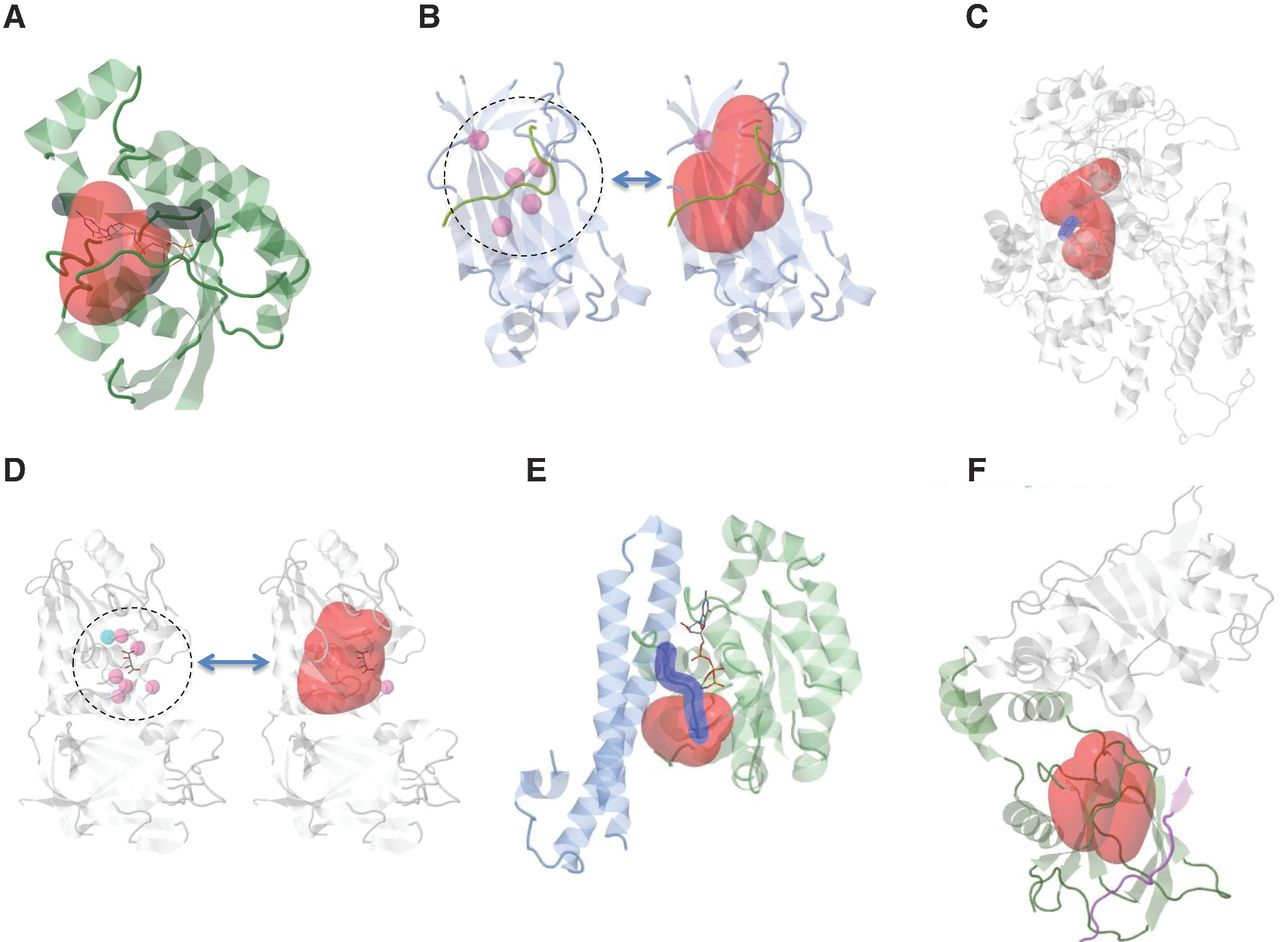
\includegraphics[width=0.9\linewidth]{figures/chapter5/hotmaps_examples.jpg}
  \caption[HotMAPS hotspot regions overlap and are proximal to important functional sites.]{HotMAPS hotspot regions overlap and are proximal to important functional sites. A, HNSCC hotspot region (red) in RAC1 (green) and GTP/GDP-binding residues (dark gray; PDB 2FJU). B, PRAD hotspot region (red) in SPOP-substrate complex (PDB 3HGH) with SPOP (blue) and H2AFY substrate (green). Left, five residues (pink) that when mutated show strongly reduced affinity for substrate. C, BLCA hotspot region (red) in ERCC2 (gray) shown on theoretical model of ERCC2 helicase ATP-binding domain. The hotspot is proximal to the DEAH box (blue), a highly conserved motif containing residues that interact with Mg2+ and are critical for ATP-binding and helicase activity. D, UCEC hotspot region (red) in PTEN (PDB 1D5R) with active site phosphocysteine residue (blue), residues when mutated annotated to reduce phosphatase activity (pink). E, STAD hotspot region (red) in RHOA with a GTP analog bound (sticks; PDB 1CXZ). GTP-binding residues and effector region, dark blue. F, KIRC hotspot region (red) in VHL-TCEB1-TCEB2 complex, bound to HIF1A peptide (PDB 4AJY). Proximity to the interaction site of VHL (green) and HIF1A (blue) suggests possible decreased ubiquitination of HIF1A, resulting in increased protein expression of HIF1A. TCEB1 and TCEB2, gray.}
  \label{fig:hotmaps_examples}
\end{figure}

\subsection{RAC1 hotspot in squamous head and neck cancer}
RAC1 is a Rho GTPase important in signaling systems that regulate the organization of actin cytoskeleton and cell motility. The hotspot overlaps the GTP/GDP-binding site and could impact regulation of normal RAC1 cycling between GTP- and GDP-bound states (\autoref{fig:hotmaps_examples}A). It contains a previously identified recurrent mutation in melanoma (P29S), which dysregulates RAC1 by a fast cycling mechanism \cite{RN124}.

\subsection{SPOP hotspot in prostate cancer (PRAD)}
SPOP is the substrate recognition component of a cullin3-based E3 ubiquitin-protein ligase complex, which targets multiple substrates for proteasomal degradation. The hotspot overlaps with a binding groove harboring five residue positions (pink) where mutagenesis has strongly reduced affinity for the substrate (annotated in the UniProtKB) (\autoref{fig:hotmaps_examples}B).

\subsection{ERCC2 hotspot in bladder cancer}
ERCC2 is an ATP-dependent helicase that is part of the protein complex TFIIH involved in RNA polymerase II transcription and nucleotide excision repair (NER). I identified a hotspot region, proximal to the DEAH box, a highly conserved motif containing residues that interact with Mg2+ and are critical for ATP binding and helicase activity (\autoref{fig:hotmaps_examples}C). This proximity suggests that the hotspot mutations could disrupt ATPase activity and yield defective NER \cite{RN125}.

\subsection{PTEN hotspot}
PTEN is a phosphatase for both proteins and phosphoinositides, and it removes a phosphate from PIP3, critical for signaling to AKT. The hotspot region identified in endometrial cancer (UCEC) spans two functionally important loops in the protein (P and WPD loops) at the boundary of the active site pocket (\autoref{fig:hotmaps_examples}D). Residues in these loops are critical for catalysis (blue dot) and are important for the P-loop's conformation. Mutagenesis of residues in the WPD loop reduces phosphatase activity and increases colony formation in cell culture \cite{RN126}. Pink dots show residues that impact phosphatase activity.

\subsection{RHOA hotspots}
RHOA is a small GTPase oncogene, and like RAC1 is a member of the Ras superfamily \cite{RN127}. I identified hotspot regions in bladder cancer (BLCA), head and neck squamous cell cancer (HNSCC), and stomach adenocarcinoma (STAD). The hotspot regions overlap with the RHOA effector region, a highly conserved motif that is involved in Ras superfamily signaling with downstream effector proteins (\autoref{fig:hotmaps_examples}E). The regions are immediately proximal to a magnesium ion, which has been implicated in regulating the kinetics of Rho family GTPases \cite{RN128}.

\subsection{VHL hotspot (KIRC)}
VHL is a component of an E3 ubiquitin protein ligase complex, and it ubiquitinates the OG transcription factor HIF1A, targeting it for proteasomal degradation \cite{RN129}. One impact of VHL loss of function with failure to ubiquitinate HIF1A is increased protein expression of HIF1A. The hotspot region is proximal to its interaction site with HIF1A and could potentially have an impact on this interaction (\autoref{fig:hotmaps_examples}F). The TCGA kidney cancer (KIRC) samples were stratified on the basis of their missense mutation status: VHL hotspot, non-hotspot, or no missense (WT). HIF1A protein expression was not significantly different between VHL non-hotspot and VHL WT groups (P = 0.5; Mann-Whitney U test), but was significantly higher between VHL hotspot and VHL WT groups (P = 0.03; Mann-Whitney U test). This result is consistent with a special role for VHL hotspot missense mutations in regulating HIF1A protein expression. However, increased HIF1A expression in these KIRC samples is likely impacted by additional genetic and other factors. I might see a substantially lower P value if VHL hotspot mutations were the only cause of the observed increase. Also, there are many VHL missense mutations outside of the hotspot region, and it is likely that several of these also have a functional impact. In particular, several of them are at the interface of VHL and the TCEB1 and TCEB2 in the complex and could impact VHL/TCEB binding.

\section{Conclusions}

I systematically identify 3D missense hotspot regions using TCGA somatic mutation data from 6,594 samples in 23 tumor types. HotMAPS identified 107 unique regions and 216 cancer type-specific regions. This catalog enables assessment of how the specific missense mutations in a hotspot contribute to cancer-associated molecular mechanisms. Unlike many machine learning algorithms, the visualization of HotMAPS region with protein structure allows model interpretability by biologists with domain knowledge of a particular protein.

At the time of publication, several other algorithms were published which also supported the notion that mutational clustering in protein structure was advantageous \cite{RN133, RN131, RN132}. In a comparison from \cite{RN133}, HotMAPS had performance equivalent to other top methods on discriminating likely driver missense mutations from an in vivo experiment. The HotMAPS algorithm does have similarities with the DBSCAN algorithm \cite{RN117}, which is also based on using density estimates for clustering. However, DBSCAN does not have a statistically principled criterion for controlling false discoveries. 

Although recurrent missense mutations have long been known to occur in both oncogenes and tumor suppressor genes \cite{RN107}, they have been observed more frequently in oncogenes. I show that there are systematic differences in hotspot regions found in oncogenes and tumor suppressor genes. Oncogene regions are smaller, less mutationally diverse, more evolutionarily conserved, and more solvent accessible than tumor suppressor gene regions. Tumor suppressor gene regions are more likely to harbor mutations that may impact protein stability through changes in hydrophobicity or volume. Potential explanations for these differences are that there are more ways to lose the function of a protein than to gain function \cite{RN130}. Loss-of-function tumor suppressor mutations can occur at many residue positions and involve many types of amino acid residue substitutions, while oncogene mutations will occur at a few functionally important positions and involve fewer substitution types.


%!TEX root = root.tex

\chapter{CHASMplus: enhanced context reveals the scope of somatic missense drivers in human cancers}
\label{chap:ch6}
\chaptermark{CHASMplus}

\section{Introduction}
In previous chapters, I have shown large-scale sequencing studies of patient cohorts have enabled identification of many genes or regions that are cancer drivers. However, not every mutation in a driver gene or region is necessarily a driver of cancer; thus, requiring methods to discriminate whether an individual mutation is a driver or passenger.

The most common approach has been to apply machine learning to predict the cancer driver status of individual missense mutations by leveraging features characterizing a mutation, e.g., inter-species evolutionary conservation, features of the local protein environment, molecular function annotations, and biophysical characterizations of the amino acid substitution. Cancer-focused machine learning methods have previously tried to enhance performance by training cancer type specific models \cite{RN36, RN29} or boosting data with synthetic passenger missense mutations \cite{RN29}.  Unfortunately, a recent systematic study comparing 15 such methods concluded that none of them were sufficiently reliable for experimental or clinical follow-through \cite{RN134, RN136}. I and others have hypothesized that determining the impact of missense mutations requires proper context \cite{RN47}, which has not been sufficiently leveraged in a comprehensive manner in the current generation of methods.

In this chapter, I present a new driver missense mutation prediction method, CHASMplus, that uses machine learning to integrate missense mutation context at multiple scales. The new CHASMplus consistently outperforms comparable methods, including the original CHASM, on eight different benchmark sets -- including in vitro experiments, in vivo experiments and literature benchmarks. Encouraged by these results, I applied CHASMplus to 8,657 The Cancer Genome Atlas (TCGA) samples from 32 cancer types to systematically identify driver missense mutations.

\section{CHASMplus algorithm}

\subsection{Overview}
CHASMplus uses the Random Forest algorithm to discriminate driver somatic missense mutations (referred to hereafter as missense mutations) of human cancers from passenger missense mutations (Online Methods). A Random Forest is an ensemble of many randomized decision trees (see \autoref{ch:chp3}) \cite{RN41, RN40}. Each tree is trained on a random selection of training set examples and candidate features, via a recursive splitting process \cite{RN89}(\autoref{fig:chasmplus_overview}A). CHASMplus is trained using somatic mutation calls from The Cancer Genome Atlas (TCGA) covering 8,657 samples in 32 cancer types.  Because there is no gold standard set of driver and passenger missense mutations, I developed a semi-supervised approach to assign class labels to missense mutations, taking advantage of Random Forest robustness to noisy class labels.  Briefly, class labels are assigned so as to enrich the positive class for driver missense mutations (\autoref{fig:chasmplus_overview}B). CHASMplus training is done with a rigorous gene holdout cross-validation protocol to avoid overfitting, by ensuring all mutations within a gene are within the same fold \cite{RN128, RN137}. Therefore, missense mutations are never scored by a Random Forest trained on any missense mutation harbored by the same gene.  Finally, predicted scores from CHASMplus are weighted by the 20/20+ driver gene score, producing gene-weighted (gwCHASMplus) scores (\autoref{fig:chasmplus_overview}B).

\begin{figure}
  \centering
  \makeatletter
  \let\@currsize\normalsize
  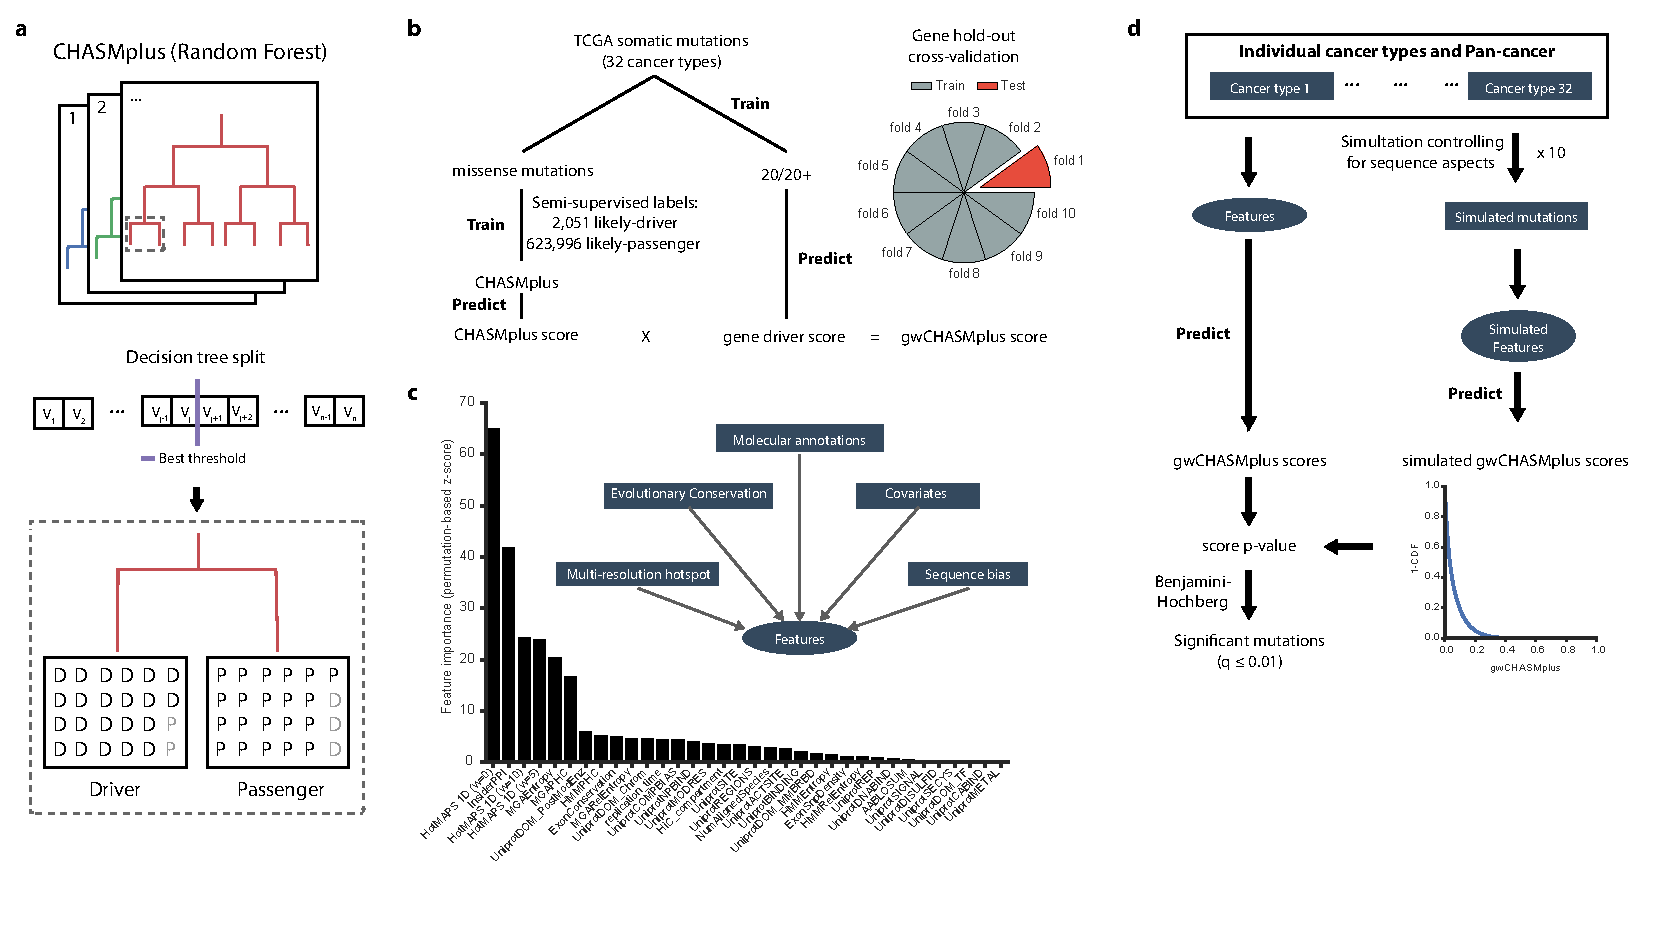
\includegraphics[width=\linewidth]{figures/chapter6/chasmplus_overview.pdf}
  \caption[Overview of CHASMplus algorithm.]{Overview of CHASMplus algorithm. a) CHASMplus predicts driver somatic missense mutations by using a random forest algorithm, consisting of an ensemble of decision trees. Each decision tree is constructed by selecting a random set of examples and features and recursively splitting examples by the best split criterion. b) Diagram of training and testing procedure by CHASMplus. c) Features with a net-positive feature importance by CHASMplus according to a permutation adjusted z-score. Boxed text indicates broad feature categories that were important. d) Diagram of how CHASMplus identifies statistically significant driver somatic missense mutations in each of the 32 cancer types individually and in aggregate (pan-cancer).}
  \label{fig:chasmplus_overview}
\end{figure}

\subsection{Semi-supervised training labels}
Using the TCGA mutation dataset, I established training labels with a semi-supervised approach, designed to minimize bias (\autoref{fig:chasmplus_flow_diagram}A). The positive class (likely-driver missense mutations) was selected by the following criteria: 1) missense mutations had to occur in a curated set of 125 pan-cancer driver genes \cite{RN25}; 2) for each of the 32 TCGA cancer types, missense mutations found in that cancer type had to occur in a significantly mutated gene for that cancer type according to MutSigCV v1.4 \cite{RN14}. I ran MutSigCV using recommended settings and a full sequencing coverage file (\url{http://archive.broadinstitute.org/cancer/cga/mutsig}).  Importantly, MutSigCV v1.4 only assess the total number of mutations in a gene, and not any characteristics of those mutations; thus, I avoid making strong assumptions about the properties of a particular driver mutation; 3) missense mutations had to occur in samples with relatively low mutation rate (less than 500 mutations, half the minimum hypermutator threshold).  This filter was intended to limit the number of passenger mutations mislabeled as drivers.  The negative class (likely-passenger missense mutations) consisted of the remaining missense mutations in the TCGA mutation set.  For training purposes, I only used unique mutations to avoid double counting a mutation seen more than once. If, however, the same mutation consequence observed in different cancer types had contradictory labels, I regarded the mutation as a driver because mutation recurrence is often cited as supportive evidence for a cancer driver role. This established a set of 2,051 likely-driver missense mutations and 623,996 likely-passenger missense mutations, for which I found sufficient annotation to compute our selected features.

\begin{figure}
  \centering
  \makeatletter
  \let\@currsize\normalsize
  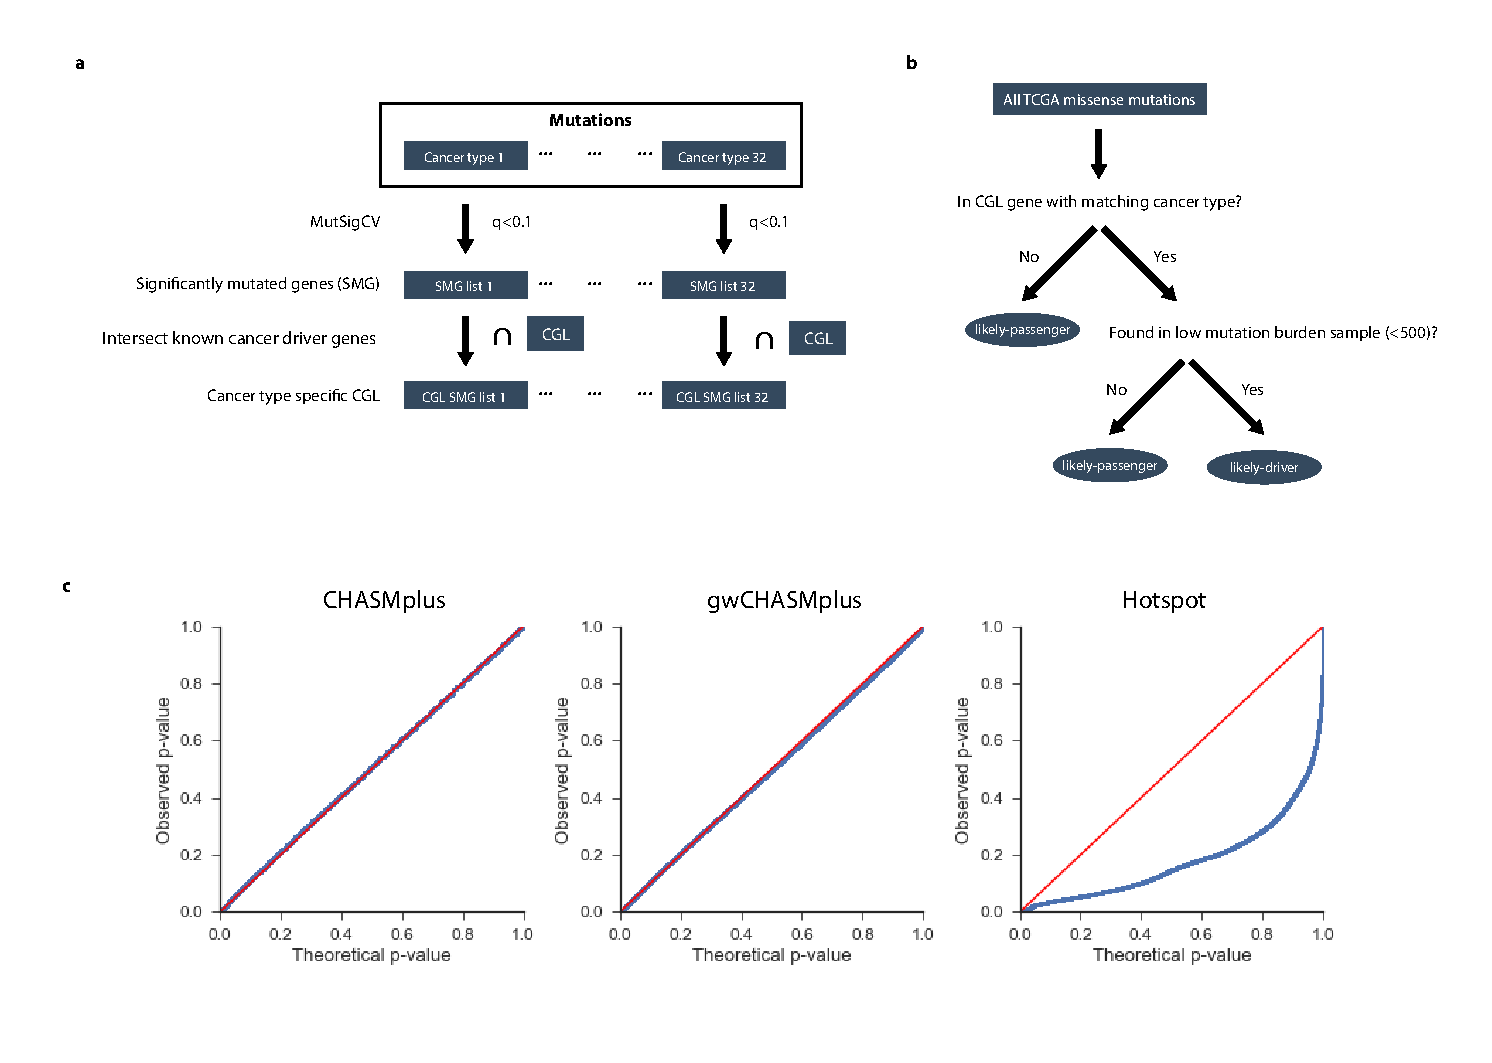
\includegraphics[width=0.9\linewidth]{figures/chapter6/chasmplus_flow_diagram.pdf}
  \caption[Training set labeling procedure and calibration of statistical model]{Training set labeling procedure and calibration of statistical model. a) Diagram demonstrating how the cancer type specificity of Cancer Genome Landscape (CGL) genes were determined. b) Somatic missense mutations were labeled either as "likely-passenger" or "likely-driver" based on a semi-supervised approach using two steps: overlap with previously known genes from CGL in a cancer type specific manner and samples with low mutation burden. c) QQ plot of observed p-values for a method (blue line) compared to theoretically expected under the null hypothesis (red line). All mutations in genes found in the Cancer Gene Census were removed to eliminate possible driver mutations in this comparison. CHASMplus represents unweighted CHASMplus scores, gwCHASMplus represents gene weighted CHASMplus scores, and Hotspot is a previous codon-level mutation hotspot detection method.}
  \label{fig:chasmplus_flow_diagram}
\end{figure}

\subsection{Features}
CHASMplus scores benefit from representation of missense mutation context at multiple scales. The Random Forest was trained on 95 features, and the 34 features with a net positive feature importance are shown in \autoref{fig:chasmplus_overview}C. Important features assess five broad categories: multi-resolution missense mutation hotspots (HotMAPS 1D algorithm \cite{RN60}), evolutionary conservation/human germline variation, molecular function annotations (e.g., protein-protein interface annotations from \cite{RN139}), sequence biased regions, and gene-level covariates (e.g., replication timing). Missense mutation context is further represented by the 20/20+ driver score of the gene harboring the missense mutation and the specific cancer type in which it was observed.  While gene-level features have been previously applied to missense mutation driver prediction \cite{RN35}, to my knowledge, this is the first time that gene-level and missense mutation-level driver scores have been coupled in a cancer type-specific manner.  

\subsection{Statistical significance}
CHASMplus can also evaluate the statistical significance of cancer type-sepcific predictions for each of 32 cancer types from The Cancer Genome Atlas (TCGA), and pan-cancer predictions for all TCGA cancer types in aggregate (\autoref{fig:chasmplus_overview}D). Because Random Forests do not intrinsically include hypothesis testing techniques, I used simulated mutations to assess the statistical significance of scores. P-values were estimated from a simulated null distribution, controlling for sequence composition, and corrected for multiple testing with the Benjamini-Hochberg method (see \autoref{sec:monte_carlo}). The resulting P-value distributions suggest our statistical model is well calibrated (\autoref{fig:chasmplus_flow_diagram}B).  Well-calibrated P-values enable quantitative estimates of false discovery rate and thus inform a user about how to select a suitable score threshold for predicted driver missense mutations.

\section{CHASMplus dramatically improves identification of  missense mutation drivers}
I next sought to compare the performance of CHASMplus on seven mutation-level benchmarks with respect to 12 comparable methods: VEST \cite{RN30}, CADD \cite{RN34}, FATHMM cancer \cite{RN39}, SIFT \cite{RN116}, MutationAssessor \cite{RN38}, REVEL \cite{RN32}, MCAP \cite{RN33}, ParsSNP \cite{RN35}, CHASM \cite{RN29}, Polyphen2 \cite{RN28}, transFIC \cite{RN31} and CanDrA \cite{RN36}. Scores were obtained by means made available by each of the methods. 

My benchmarks fall under three broad categories: in vitro experiments, high throughput in vivo screens, and curation from published literature.  Each of these categories has weaknesses, but, in aggregate, they span multiple scales of evaluation and amount of supportive evidence (\autoref{chasmplus_benchmark}A). For example, several benchmarks are limited to one or a few well-established driver genes, while others are exome-wide, but lack experimental support. A range of benchmarks is critical because missense mutations with the most established experimental support for a driver role tend to be in a few well-understood cancer driver genes.  However, limiting benchmarking to these genes makes it difficult to assess the generalizability of a method's performance to missense mutations in other genes. All benchmark evaluations used the area under the Receiver Operating Characteristic Curve (auROC) as a metric (\autoref{chasmplus_benchmark}B).  Overall, CHASMplus had a mean auROC of 0.09 higher than the next best method. This common metric is used in machine learning to describe how well predictions separate two classes without a priori selecting a score threshold, which for many methods is not well defined \cite{RN140}. In our assessment, the two classes represent likely driver and passenger missense mutations. In general, auROC values range from 0.5 (random prediction performance) to 1.0 (perfect).

\begin{figure}
  \centering
  \makeatletter
  \let\@currsize\normalsize
  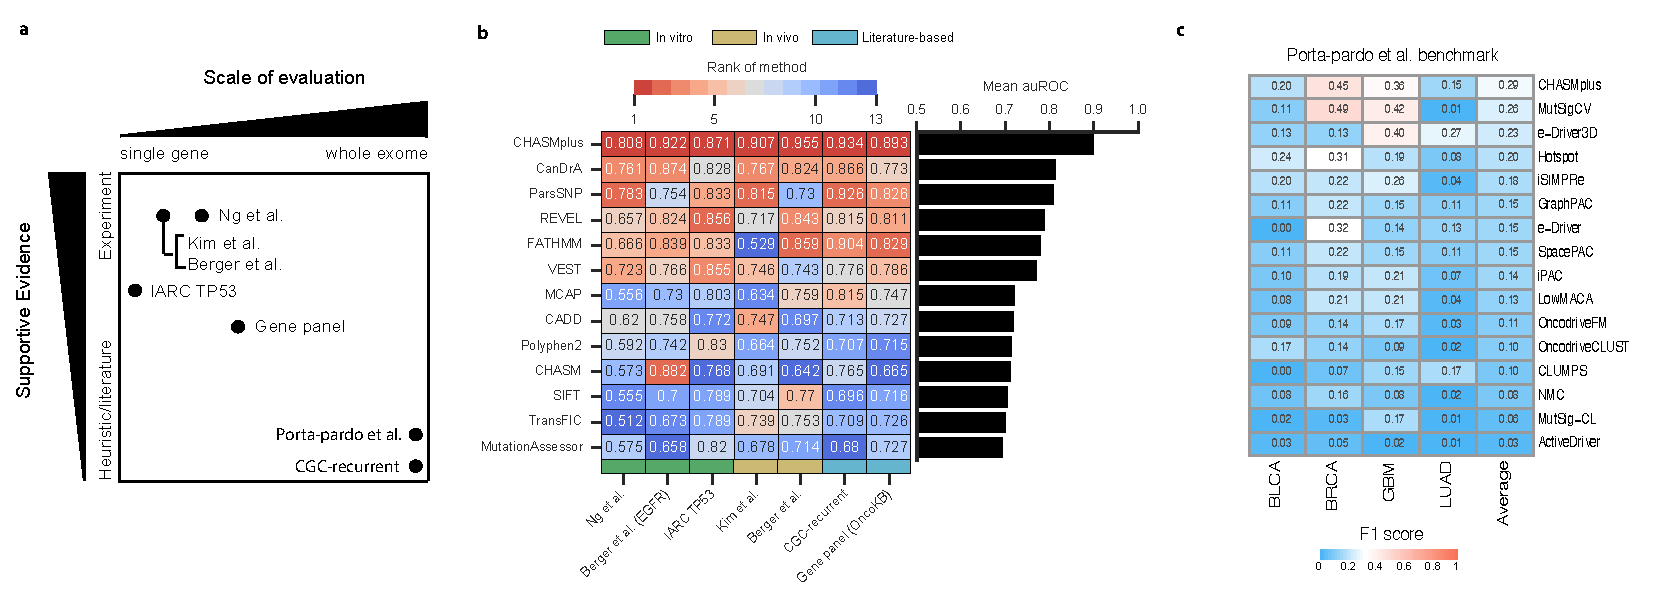
\includegraphics[width=0.9\linewidth]{figures/chapter6/chasmplus_benchmark.pdf}
  \caption[Cancer driver prediction benchmark.]{Cancer driver prediction benchmark. a) Conceptual diagram of how 8 benchmarks compare in terms of the scale of evaluation and amount of supportive evidence. b) A heatmap showing performance measured by the area under the Receiver Operating Characteristic Curve (auROC) on the 7 mutation-level benchmarks (shown in text). The color scale from red to blue indicates methods ranked from high to low performance.  Benchmarks are categorized by in vitro (green), in vivo (yellow), and literature-based benchmarks (turquoise). The bar graph shows the mean auROC across the benchmarks. c) Heatmap showing performance (F1 score) on a cancer type specific benchmark. The overall performance on four cancer types (BLCA, BRCA, GBM, and LUAD) is measured by the average F1 score (right column).}
  \label{fig:chasmplus_benchmark}
\end{figure}

I used three benchmarks based on in vitro experiments. The first was a set of missense mutations assessed by an assay of cell viability in two growth-factor dependent cell lines, Ba/F3 and MCF10A (pro-B and breast epithelium cell lines), covering 747 mutations in 48 genes \cite{RN187}. CHASMplus had significantly higher performance than the next best performing method (ParsSNP) (p<0.05, delong test). In the second benchmark, an in vitro assay of EGFR resistance to erlotinib from missense mutations observed in lung adenocarcinoma \cite{RN141}, CHASMplus (auROC=0.92) outperformed all other methods, with the next best method (CanDrA) having an auROC of 0.87.  CHASMplus auROC was significantly better than that of 7 of the methods tested (p<.05, delong test).  For the remaining 5 methods, the improvement was not significant, possibly due to lack of power given the small number of mutations (n=75) tested in the assay.  In the third benchmark, an assay of reduced transactivation (<50\% WT, median of 8 targets) in TP53 from the IARC database (n=2,314 mutations)\cite{RN142}, CHASMplus significantly outperformed the next best method (REVEL) (p=0.02, delong test).

To investigate whether CHASMplus would also perform well when compared to results of in vivo experiments, I considered two benchmarks based on pooled in vivo screens in mice that assessed mutation driver status by fitness in a competition assay.  The first was performed from mutations observed in lung cancers (44 missense mutations) \cite{RN141} and the second from mutations observed in 27 cancer types (71 missense mutations) \cite{RN143}. CHASMplus had the highest auROC of the 13 tested methods on both benchmarks, with an increase in auROC by 0.09 and 0.1, respectively, compared to the next best methods (ParsSNP in the first benchmark and FATHMM in the second). The increase was significant in the second larger, benchmark (p=0.03, delong test, n=72), but not in the first, which may be the result of the smaller sample size.  In the first benchmark, CHASMplus was significantly better than 9 out of 12 tested methods (p<0.05, delong test, n=44).

Experimental testing of mutations across large number of genes or the whole exome is currently not feasible. Therefore, evaluation of CHASMplus at larger scales relied on two benchmarks based on literature and database curation. The first benchmark in this category labeled recurrent missense mutations within genes in the Cancer Gene Census \cite{RN97} as drivers. I found that the gene weighted CHASMplus scores (auROC=0.934) were substantially better at this whole exome-wide prioritization task compared to the unweighted CHASMplus scores (auROC=0.893) (p<2.2e-16, delong test). CHASMplus scores were also significantly better than the next best method (ParsSNP) (p=0.001, delong test). The second benchmark was derived from a large driver gene panel (MSK-IMPACT, 414 genes) and 10,130 sequenced cancer patients \cite{RN145}.  Missense mutations were labeled as drivers if they were annotated as such in OncoKB \cite{RN144}, a knowledge-base that aggregates known literature. CHASMplus significantly outperformed all other methods, the nearest being ParsSNP (p=7e-14, delong test). 

\section{CHASMplus improves identification of cancer type specific driver genes}
I evaluated the performance of CHASMplus on identifying cancer-type specific driver genes, using a previously published benchmark and assessment of 15 computational methods designed for this purpose \cite{RN52}. The 15 methods are: Hotspot \cite{RN16}, NMC \cite{RN106}, OncodriveCLUST \cite{RN54}, MutSig-CL \cite{RN14}, iSiMPRe \cite{RN150}, iPAC \cite{RN15}, GraphPAC \cite{RN151}, SpacePAC \cite{RN152}, CLUMPS \cite{RN105}, e-Driver \cite{RN153}, e-Driver3D \cite{RN45}, ActiveDriver \cite{RN154}, LowMACA \cite{RN155}, OncodriveFM \cite{RN53}, and MutSigCV \cite{RN13}. Genes were labeled by their designations in the Cancer Gene Census as a cancer driver gene for a specific cancer type. Out of the 4 cancer type cohorts assessed (BLCA, BRCA, GBM, and LUAD), CHASMplus had the highest average F1 score, a balance between precision and recall that was used as a performance metric by \cite{RN52} (\autoref{fig:chasmplus_benchmark}C). I additionally note that of the methods tested, CHASMplus was the only one not primarily designed to predict driver genes that had high recall (average recall=.45) while maintaining precision (average precision=.23). 

\section{CHASMplus identified both common and rare cancer drivers}
Certain cancer driver mutations primarily occur in a specific cancer type, while others appear in many cancer types.  The power to detect driver mutations, which occur at low frequency in many cancer types, is increased when many cancer types are aggregated, known as a pan-cancer analysis. Conversely, driver mutations, which are specific to a particular cancer type, are best identified when cancer types are analyzed individually \cite{RN59}. Using CHASMplus, I identified 3,527 unique missense mutations as statistically significant drivers by pan-cancer analysis at an estimated false discovery rate of 1\%. When applied to each cancer type individually, the number found significant varied substantially from 8 in thymoma to 572 in bladder urothelial carcinoma with a median of 78 (\autoref{fig:chasmplus_tcga}A). The median overlap with literature-based oncogenicity annotation from OncoKB was 53\%, suggesting 47\% of the driver missense mutations identified by CHASMplus either have not been previously characterized or not sufficiently characterized for inclusion in OncoKB.  While OncoKB missense mutation annotations are not cancer-type specific, the genes with highest frequencies of cancer-type specific driver missense mutations identified by CHASMplus have well-known roles in cancer \cite{RN5} (\autoref{fig:chasmplus_tcga}B). 

\begin{figure}
  \centering
  \makeatletter
  \let\@currsize\normalsize
  \includegraphics[width=0.9\linewidth]{figures/chapter6/chasmplus_tcga.pdf}
  \caption[Cancer driver prediction benchmark.]{Discovery of driver somatic missense mutations. a) Bar graphs showing the number of unique driver somatic missense mutations (top) and the proportion previously known in OncoKB, a literature curated database (bottom). b) Heatmap of the top 25 genes containing the most frequent driver somatic missense mutations in TCGA across the cancer type specific analyses. Shown are the percentage of samples that are mutated. c) Proportion of overall frequency of driver somatic missense mutations found in rare ($<$1\% of samples or singleton mutations), intermediate (1-5\%), and common ($>$5\%) driver somatic missense mutations. Correspondingly shown as light to dark blue. d) Structure of the Phosphatase 2A holoenzyme (PDB 2IAE). e) Structures of the ERBB2 extracellular domain (left, PDB 2A91) and kinase domain (right, PDB 3PP0).}
  \label{fig:chasmplus_tcga}
\end{figure}

The long tail hypothesis, proposed from examining overall mutation frequency of driver genes \cite{RN27, RN35}, suggests there are many rare drivers. However, the overall mutation frequency of a gene does not account for the confounding presence of passenger mutations within a driver gene. From our mutation-level analysis, I observed that the relative prevalence of rare ($<$1\% of samples), intermediate (1-5\%), and common ($>$5\%) driver missense mutations varied substantially among cancer types (\autoref{fig:chasmplus_tcga}C). For example, uveal melanoma was dominated by common driver missense mutations (88\%), while head and neck squamous cell carcinoma (HNSC) was dominated by rare driver missense mutations (63\%). Overall, the proportion of rare driver mutations identified from our pan-cancer analysis by CHASMplus (35.4\%) is approximately 4-fold higher than indicated by a computational method using hotspot codons (8.2\%, P$<$2.2e-16, Fisher's exact test) \cite{RN23}.   Interestingly, the proportion of rare driver missense mutations identified by CHASMplus is close to the proportion of common driver missense mutations (35.5\%).  

Rare driver missense mutations exist not only in rare driver genes, but also may be spatially proximal in protein structure to common driver missense mutations. For example, the protein phosphatase PPP2R1A, which has been implicated as a tumor suppressor gene in many tumor types \cite{RN57}, contained common driver missense mutations in our pan-cancer analysis at residue positions 179 and 183, which is located at the protein interface composing the phosphatase 2A complex (\autoref{fig:chasmplus_tcga}D). It also had a much broader set of rare drivers throughout the protein interface, such as R105Q and R459C.  Similarly, CHASMplus identified common driver missense mutations (S310A/F/Y) in the extracellular domain of the well-known oncogene ERBB2, but also finds rare driver missense mutations in both the extracellular and kinase domain (e.g., L313V and R678Q) (\autoref{fig:chasmplus_tcga}E). This is supportive of previous experimental work implicating rare cancer driver mutations in common cancer driver genes \cite{RN4}.

\section{Mutation hotspot detection has limited power}
A codon or small region of protein sequence or structure where recurrent mutations are observed is known as a hotspot.  Similar to statistical methods for driver gene detection, hotspot detection identifies an excess number of mutations compared to expectation. using a large number of cancer samples.  I asked whether, given current cohort sizes, codon-based hotspot detection had sufficient statistical power to identify rare driver mutations.  I assessed the number of samples required to detect driver mutations across a range of frequencies (proportion of samples in which a mutation occurs) and somatic background mutation rates. In \autoref{fig:chasmplus_power}A, each of the 32 TCGA cancer types is placed according to its sample size and background mutation rate, relative to six curves which represent the required sample size to detect driver mutations of a certain frequency, with 90\% power, using hotspot detection.  For example, the TCGA Cervical Squamous Cell Carcinoma and Endocervical Adenocarcinoma (CESC) cohort has 274 samples and a background mutation rate of 3.5 mutations/Mb.  This sample size is sufficient to detect driver mutations that occur in ~2\% of the samples with 90\% power. 

\begin{figure}
  \centering
  \makeatletter
  \let\@currsize\normalsize
  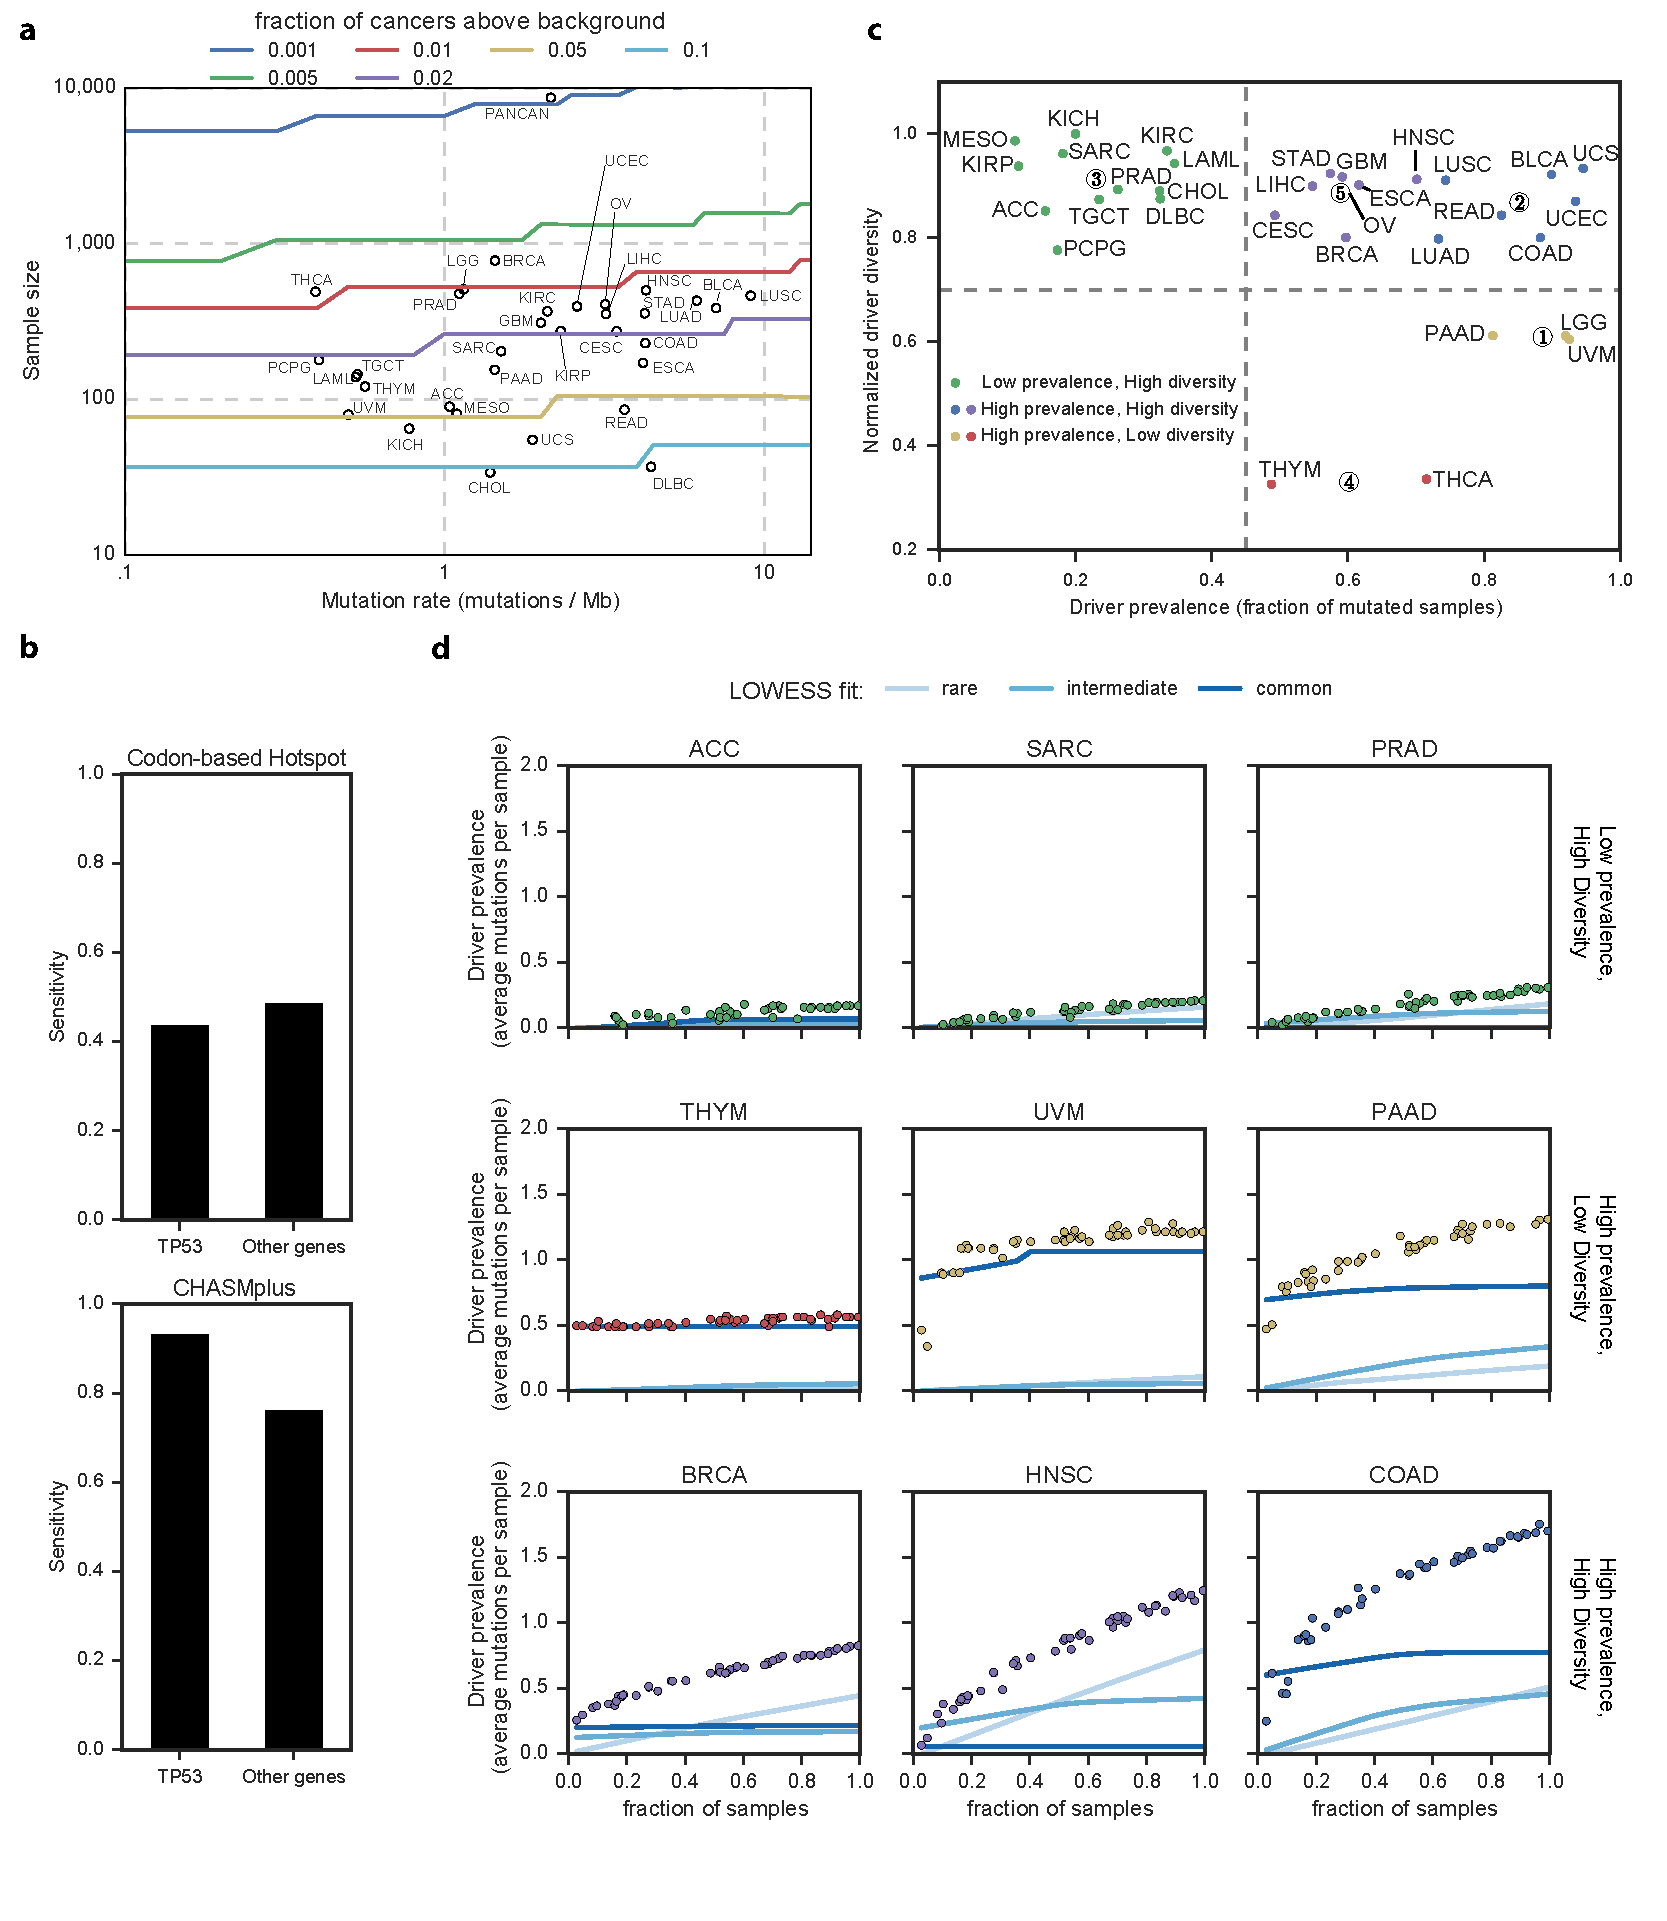
\includegraphics[width=0.9\linewidth]{figures/chapter6/diversity_and_saturation.pdf}
  \caption[Saturation and characteristics of driver somatic missense mutations.]{Saturation and characteristics of driver somatic missense mutations. a) Statistical power to detect significantly elevated non-silent mutations for individual codons as a function of sample size and mutation rate. Circles represent each cancer type from the TCGA, and is placed according to sample size and median mutation rate. Curves are colored by effect size (fraction of non-silent mutated samples above the background rate). b) Bar graph comparing sensitivity to detect labeled oncogenic driver missense mutations from OncoKB between CHASMplus and a hotspot detection approach. c) Plot displaying normalized driver diversity and driver prevalence (fraction of samples mutated) for driver somatic missense mutations in 32 cancer types. K-means clustering identified 5 clusters with centroids shown as numerically designated circles. d) Prevalence of driver somatic missense mutations as a function of sample size. Lines represent LOWESS fit to different rarities of driver somatic missense mutations.}
  \label{fig:chasmplus_power}
\end{figure}

At current TCGA sample sizes, I found codon-based hotspot detection approaches were not well powered to identify driver mutations that occurred at less than 1\% frequency in most cancer types.  Exceptions were thyroid carcinoma (THCA), low grade glioma (LGG) and breast cancer (BRCA), which are seen lie above (or close to) the curve representing 1\% frequency (\autoref{fig:chasmplus_power}A).  Notably, these cohorts had large numbers of samples and low-to-medium background mutation rates.  I also found that when cancer types were aggregated in pan-cancer analysis, power to detect codon-based hotspots improved substantially, but only when the recurrent mutations were shared in more than one cancer type.  For these mutations, pan-cancer analysis using ~10,000 TCGA samples should enable detection of driver mutations at frequency as low as 0.1\%.   

In our pan-cancer analysis, CHASMplus had greater sensitivity to detect putatively oncogenic missense mutations than a recent codon-based hotspot detection method (\autoref{fig:chasmplus_power}B). I compared the missense mutations in the TCGA pan-cancer cohort that were called statistically significant by CHASMplus and those called by a hotspot method described by \cite{RN23} ($q\leq 0.01$ for both methods).  For each method, I computed the overlap with well-curated oncogenic mutations in the OncoKB database.  CHASMplus sensitivity to detect the OncoKB-labeled mutations was 0.83.  The sensitivity of the hotspot method (0.46) was significantly lower (p$<$2.2e-16, McNemar's test, n=896).  To minimize gene bias, I also repeated the analysis after excluding all 389 TP53 mutations, yielding sensitivity of 0.76 for CHASMplus and 0.49 for hotspot detection, a difference which is still statistically significant (p<2.2e-16, McNemar's test, n=507).  I believe that the increased sensitivity is the result of CHASMplus using a broad range of important features, including multi-resolution hotspot detection (\autoref{fig:chasmplus_power}C).

\section{Characterizing cancer types and the trajectory of discovery}
The diversity and prevalence of driver missense mutations varied considerably across TCGA cancer types (\autoref{fig:chasmplus_power}C).  I defined diversity with respect to the distribution of driver missense mutations across codons and prevalence with respect to the frequency of the mutations in tumor samples.  High diversity indicated mutations were broadly distributed across codons, while high prevalence indicated driver missense mutations that occurred in a large number of tumor samples. Using K-means clustering, I found that cancer types grouped into high diversity and low prevalence (12 cancer types), high diversity and high prevalence (15 cancer types), and low diversity and high prevalence (5 cancer types). These differences were not associated with intra-tumor heterogeneity or normal contamination, as assessed by mean variant allele fraction (VAF) of a cancer type (p$>$0.05, correlation test).  The differences also could not be associated only with TCGA sample size for a particular cancer type.  For example, while both pancreatic ductal adenocarcinoma (PAAD) and sarcoma (SARC) had similar sample sizes (n=155, n=204 respectively), PAAD had high prevalence and low diversity, while SARC had low prevalence and high diversity. After adjusting for sample size, I observed that the average mutation burden for a cancer type positively correlated with the prevalence of rare (but not common) driver missense mutations (R=0.63, P=4.7e-5, likelihood ratio test).

Are there substantially more cancer driver missense mutations yet to be discovered? If discovery was measured by the number of unique driver missense mutations identified, subsampling analysis showed all cancer types had a linear increase ($R^2>0.5$) with no evidence of saturation at current sample sizes (\autoref{fig:chasmplus_subsampling}).  However, I did observe substantial variability in trajectories if discovery was measured by driver prevalence (average number of driver missense mutations per cancer sample) (\autoref{fig:chasmplus_power}D), a metric which goes directly to utility of driver discovery in clinical practice (Discussion). For sarcoma (SARC), adrenocortical carcinoma (ACC), and prostate adenocarcinoma (PRAD), driver prevalence remained minimal as sample size increased.  While, in contrast, thymoma (THYM), uveal melanoma (UVM), and pancreatic ductal adenocarcinoma (PAAD) contained common driver missense mutations that could be detected by using only a few samples from the cohort, e.g., GTF2I L424H in THYM.  Due to a lack of rare or intermediate driver missense mutations, I observed THYM and UVM saturated discovery as sample size increased. Although PAAD did show a growing set of intermediate/rare driver missense mutations, the overall driver prevalence exhibited a diminishing rate of discovery. In contrast, breast (BRCA), head and neck squamous (HNSC), and colon cancers (COAD) harbored a full spectrum of driver missense mutations, with rare drivers increasing substantially as a function of sample size.

\begin{figure}
  \centering
  \makeatletter
  \let\@currsize\normalsize
  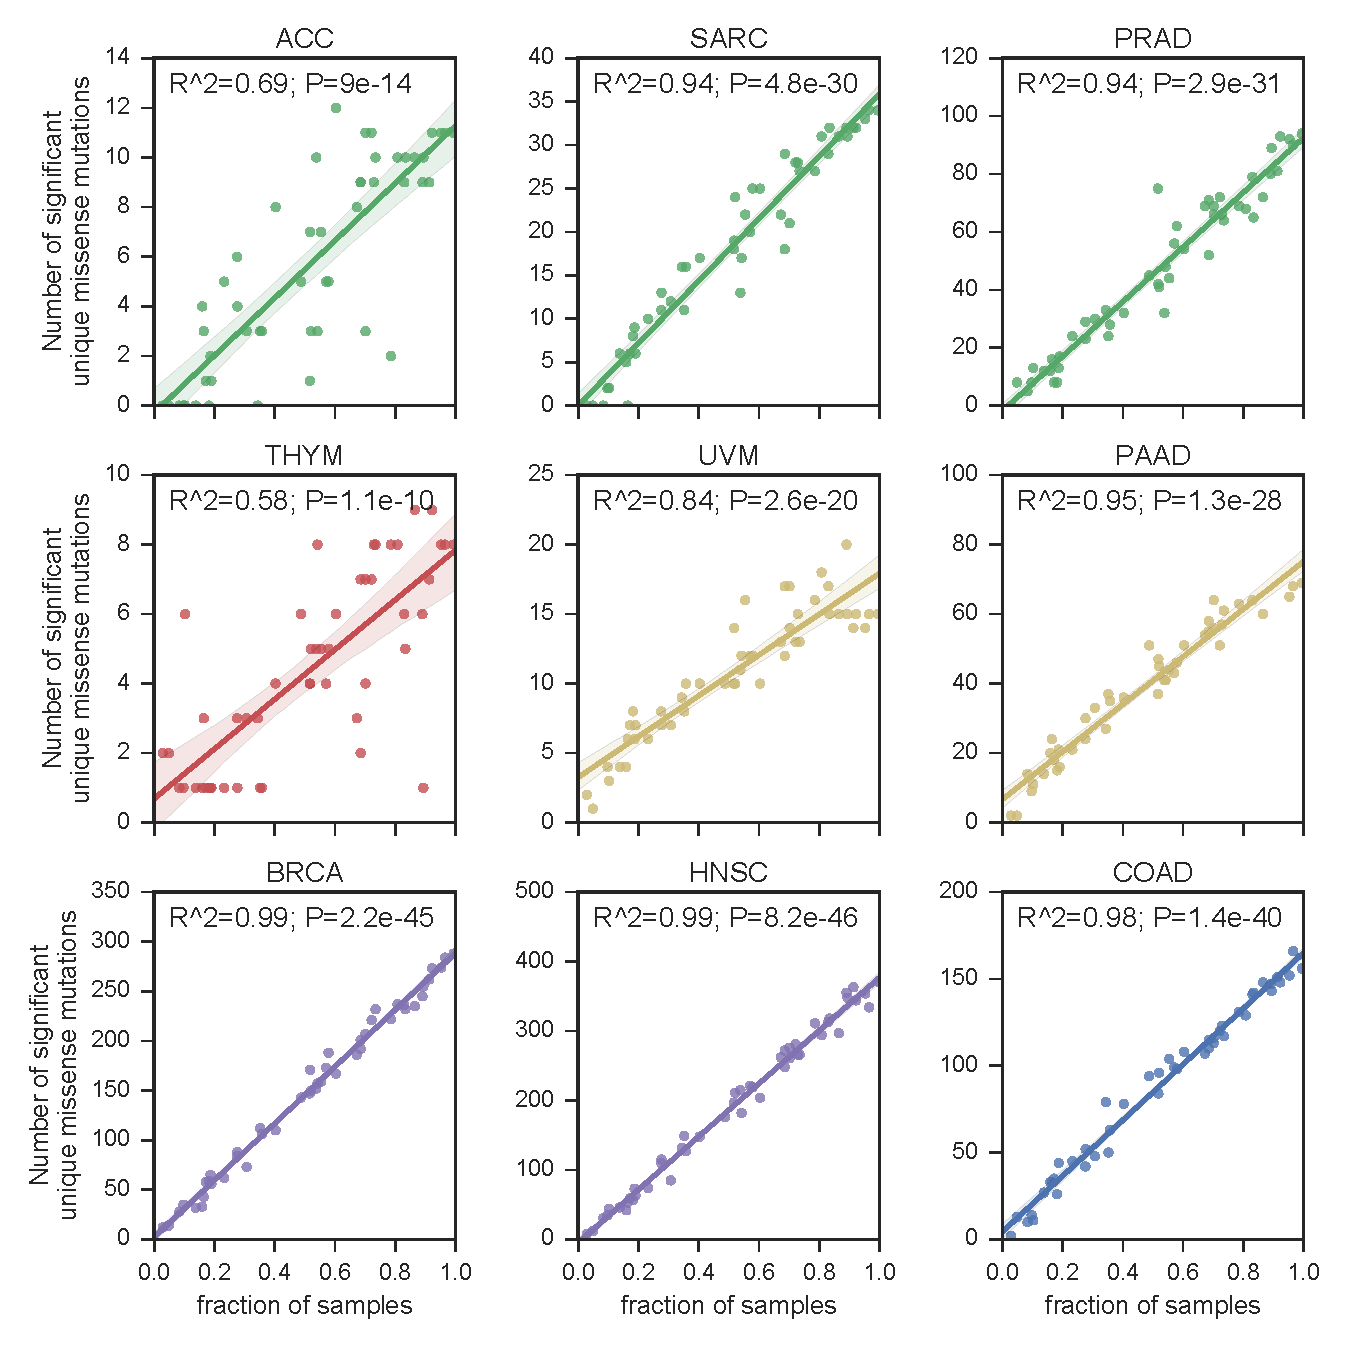
\includegraphics[width=0.9\linewidth]{figures/chapter6/sub_sampling_num_unique.pdf}
  \caption[Subsampling analysis of unique driver somatic missense mutations by CHASMplus.]{Subsampling analysis of unique driver somatic missense mutations by CHASMplus. The number of driver somatic missense mutations identified as significant by CHASMplus ($q \leq 0.01$) as a function of sample size. CHASMplus was ran on random subsets of various sizes (fraction of samples) of the full data.}
  \label{fig:chasmplus_subsampling}
\end{figure}

\section{Discussion}

CHASMplus was designed to better represent the context in which missense mutations occur, by coupling features of genetic variation in cancer - such as multi-resolution mutational hotspots and driver gene scores - with evidence of in silico functional impact.  I compared CHASMplus with 27 other computational methods, including the original CHASM, on eight benchmarks covering in vivo experiments, in vitro experiments, and literature curation, CHASMplus had the best performance at predicting drivers at each scale of evaluation - a whole exome, a targeted gene panel, and within a single gene.   Individually, none of the benchmarks was ideal.  For example, mutations in the in vitro or in vivo benchmarks, were selected by complicated study inclusion criteria and limited by resource constraints.  However, I believe that application of multiple independent benchmarks spanning a wide array of genes is the current best practice.

The long tail hypothesis \cite{RN27, RN35} posits that there are many rare driver mutations in human cancers. To assess this hypothesis, I leveraged the improvements made in CHASMplus to systematically predict driver missense mutations in 8,657 samples from the TCGA. Although individually rare, I found that rare driver missense mutations played a prominent role in aggregate, consistent with the long tail hypothesis. This result supports the critical role of assessing the prevalence of driver mutations -- failure to capture and identify rare driver mutations, which occur in aggregate at reasonable prevalences, may result in crucial missed opportunities.   Because high-throughput functional validation studies of missense mutations are not yet readily available, computational methods, like CHASMplus, are needed to prioritize mutations for low- and medium-throughput studies. 

To my knowledge, mine is the first studies to show that the prevalence and diversity of driver missense mutations is highly variable across the cancer types represented in the TCGA.  I observed that mutation burden for a cancer type positively correlated with prevalence of rare (but not common) driver missense mutations, even after correcting for sample size, suggesting that accumulating a greater number of mutations in a cancer may increase the competitiveness of rare drivers. Further investigation is warranted, because differences in the rarity of driver missense mutations could arise from a variety of factors, including the driver's strength, dependence on genetic or environmental factors, competition from other types of tumor-derived alterations, or role in cancer subtypes.

%!TEX root = root.tex

\chapter{Comprehensive discovery of driver genes and mutations in cancer}
\label{chap:ch7}
\chaptermark{Comprehensive driver discovery}

Over the past decade, The Cancer Genome Atlas (TCGA) has coordinated a monumental enterprise of data generation and genomic investigation across 33 cancer types, and numerous notable findings have emerged from this project (\url{https://cancergenome.nih.gov/publications}). The individual TCGA projects also motivated the development of many bioinformatic algorithms oriented toward discovery, characterization, and prioritization of cellular processes driving cancer based on pathways \cite{RN180}, genes \cite{RN49}, or individual variations \cite{RN181}. However, despite this remarkable progress, algorithms do not entirely agree on certain candidate cancer driver genes and mutations, necessitating continued expert curation to filter likely false positive findings. Moreover, previous PanCancer analyses \cite{RN96} have been limited to fewer cancer types and have largely avoided nominating rare driver mutations. 

\section{Mutational data set}
Mutation calls were produced by the Multi-Center Mutation Calling in Multiple Cancers (MC3) working group by harmonizing results of 7 algorithms \cite{RN167}. To reduce the false positive rate for driver gene discovery I implemented three strategies addressing known issues affecting driver detection and data quality (see Mutation calling quality control). The driver detection dataset ultimately consisted of 9,079 samples having 1,457,702 total mutations, where the number of mutations per sample was widely distributed across cancer types and was consistent with previous publications \cite{RN12, RN13, RN96}.

\subsection{Mutation calling quality control}
A publicly available MAF file (\url{https://synapse.org/MC3}) was recently compiled by the MC3 Working Group and is annotated with filter flags to highlight potential artifacts or discrepancies. This dataset represents the most uniform attempt to systematically provide mutation calls for TCGA tumors. The MC3 effort provided consensus calls from 7 software packages \cite{RN167}. Flagged artifacts include: non-exonic regions, whole-genome amplified (WGA) samples, exclusion lists, blood/tumor derived pairs, strand-bias, contamination estimations, oxo-guanine artifacts, low normal read depth, polymorphisms common in EXAC \cite{RN168}, mutations present in a panel of normal samples, non-preferred tumor normal pairs, and mutations outside the regions of interest for any caller. If a mutation was not assigned any flag and was called by 2 or more variant calling software packages, it received a 'PASS' identifier. I restricted our analysis to PASS calls with the exception of samples from OV and LAML, which were some of the earliest sequenced by TCGA. Preparations for these samples utilized whole genome amplified (WGA) DNA, an important factor in that the WGA process can induce artefactual mutations. Of the 412 OV and 141 LAML samples present in our data 347 (84\%) and 141 (100\%), respectively, had variants derived from WGA DNA. In order to maintain sample sizes and uniformity in mutation calling, I did not filter mutations containing only 'wga' filter tags from these two cancer types. I recognize multiple limitations of this mutation call set including the lack of structural variants and copy number alterations, as well as variability in sequencing depth and tumor purity. The above limitations may lead to variability in mutation detection; however, the MC3 dataset reflects the state-of-the-art in consensus mutation detection.

I also excluded highly mutated samples. These hypermutators were defined as samples with a mutation count exceeding Tukey's outlier condition, i.e. greater than 1.5 times the interquartile range above the third quartile in their respective cancer types (3Q + 1.5*IQR). Designation as a hypermutator also required the number of mutations in a sample to exceed 1000, a heuristic that limited the number of discarded samples in low mutation rate cancer types. LUAD, SKCM, and UCEC had hypermutator thresholds greater than 1000 mutations (1047, 2122, and 2545 respectively). I also excluded samples that were flagged by the analysis-working group based on pathology, but allowed \q{RNA degradation} samples to remain, as this factor is not particularly relevant for most driver prediction tools based on mutations. The final driver-discovery dataset consisted of 9,079 samples having a total of 791,637 missense mutations, 323,884 silent mutations, 96,196 3'UTR mutations, 57,900 nonsense mutations, 42,251 intronic mutations, 42,251 Frame shift deletions, 34,266 5' UTR, 21,804 splice site mutations, 19,856 RNA mutations, 11,305 frame shift insertions, 7,622 3' flanking mutations, 6,419 5' flanking mutations, 6,144 in-frame deletions, 1,362 translation start site mutations, 964 nonstop mutations, and 632 in-frame insertions.

\section{Driver gene discovery approach}
Using multiple tools can overcome numerous technical issues that confound individual statistical analyses to find driver genes, such as heterogeneous mutation rate across the genome \cite{RN13}, inflated significance for long genes \cite{RN169}, and false positive calls in cancers with high mutation rates \cite{RN70}. In the first phase, 8 different tools comprising algorithms based on mutation frequency (MuSiC2 \cite{RN43} and MutSig2CV \cite{RN14}), features (20/20+ \cite{RN70}, CompositeDriver(in preparation) and OncodriveFML \cite{RN86}), clustering (OncodriveCLUST \cite{RN54}), and externally defined regions (e-Driver \cite{RN153} and ActiveDriver \cite{RN98}) were used (\autoref{fig:driver_gene_approach}A). Each tool reported gene or mutation level scores and/or p-values along with a brief description of recommended cutoff thresholds or filters.

\begin{figure}[b!]
  \centering
  \makeatletter
  \let\@currsize\normalsize
  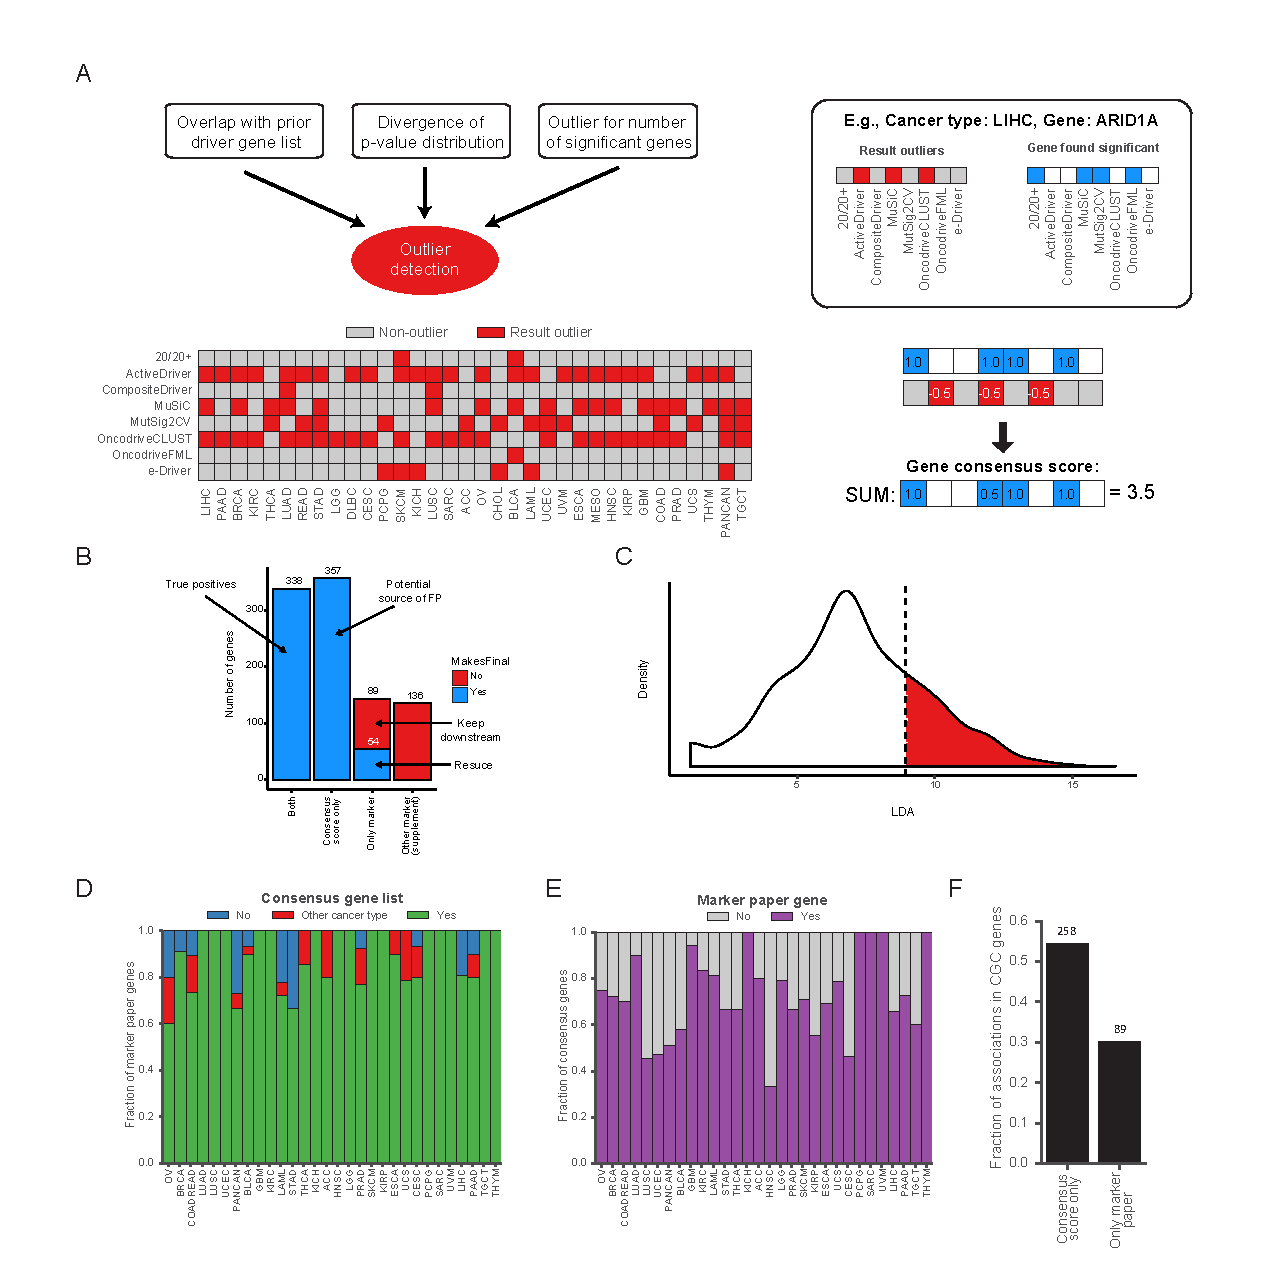
\includegraphics[width=\linewidth]{figures/chapter7/driver_gene_approach.pdf}
  \caption[Consensus Gene scores and SMG filtering.]{(Caption next page.)}
  \label{fig:driver_gene_approach}
\end{figure}
\addtocounter{figure}{-1}
\begin{figure} [t!]
  \caption[(continued) Consensus Gene scores and SMG filtering.]{(Figure previous page) Consensus Gene scores and SMG filtering. (A) Left, outlier detection was performed on a per analysis and method basis. Outliers were marked (red) based on the quasi-majority of three criteria: (1) low concordance with known cancer genes from Vogelstein et al (lower than median); (2) high divergence of p-value distribution from theoretical expectation (higher than median); and (3) abnormally high number of significant genes ($>$1.5x the interquartile range above the third quartile). The first two criteria were assessed based on the other tools within a single analysis, while the third criterion was assessed based on the same tool's results over all the individual cancer types (excluding the PanCancer analysis). Right, example calculation of the gene consensus score for ARID1A in the cancer type LIHC. A result from an outlier is down weighted, receiving a weight of 0.5 instead of 1.0. The gene consensus score is the sum of weights for tools finding that gene as significant. (B) Overlap of consensus gene list with prior TCGA marker papers. (C) Likely false positives were detected with a high Linear Discriminant Analysis (LDA) score threshold representing 90\% sensitivity for keeping associations found in Cancer Gene Census genes. LDA was trained to distinguish common false positives in exome sequencing from previous TCGA PanCancer marker papers. The LDA threshold was only applied to the potential source of false positive genes. (D) Fraction of marker paper genes highlighted in the main text that were also found in our consensus gene list. (E) Fraction of our consensus gene list found in previous TCGA marker papers.  (F) Fraction of associations found in the Cancer Gene Census (CGC) that were either found only in the consensus gene list or TCGA marker paper. }
\end{figure}

\subsection{Consensus methodology}
I identified a preliminary total of 2,101 potential drivers by taking the union of genes predicted by the eight driver-gene discovery tools.  As illustrated in \autoref{fig:driver_gene_approach}A, the increased number of false positive genes is likely due to any individual tool's capability to maintain sound statistical properties that handle a complex set of factors such as tumor heterogeneity, increased mutation rates, and variable sample sizes. I refined this list by calculating, for each gene predicted in each cancer type, a consensus score that compensated for outlier results and correlation among tools (\autoref{fig:driver_gene_approach}). The consensus score was defined as a weighted sum of the number of tools that predicted the gene to be a driver in each cancer type (see \autoref{sec:weighting}). I required a minimum of two tools to agree, where both could not be outliers (score$\geq$1.5). Although it is difficult to distinguish the overall performance improvement on a small number of held out CGC genes (\autoref{fig:gene_characteristics}A), the weighting strategy did have higher specificity (p=4.3e-8, McNemar test), which is preferable given concerns of false positives. Regardless, the consensus score performance on identifying CGC genes (\autoref{fig:gene_characteristics}A) support previous reports that merging the results from different algorithms improve cancer driver discovery \cite{RN96}. 

\begin{figure}
  \centering
  \makeatletter
  \let\@currsize\normalsize
  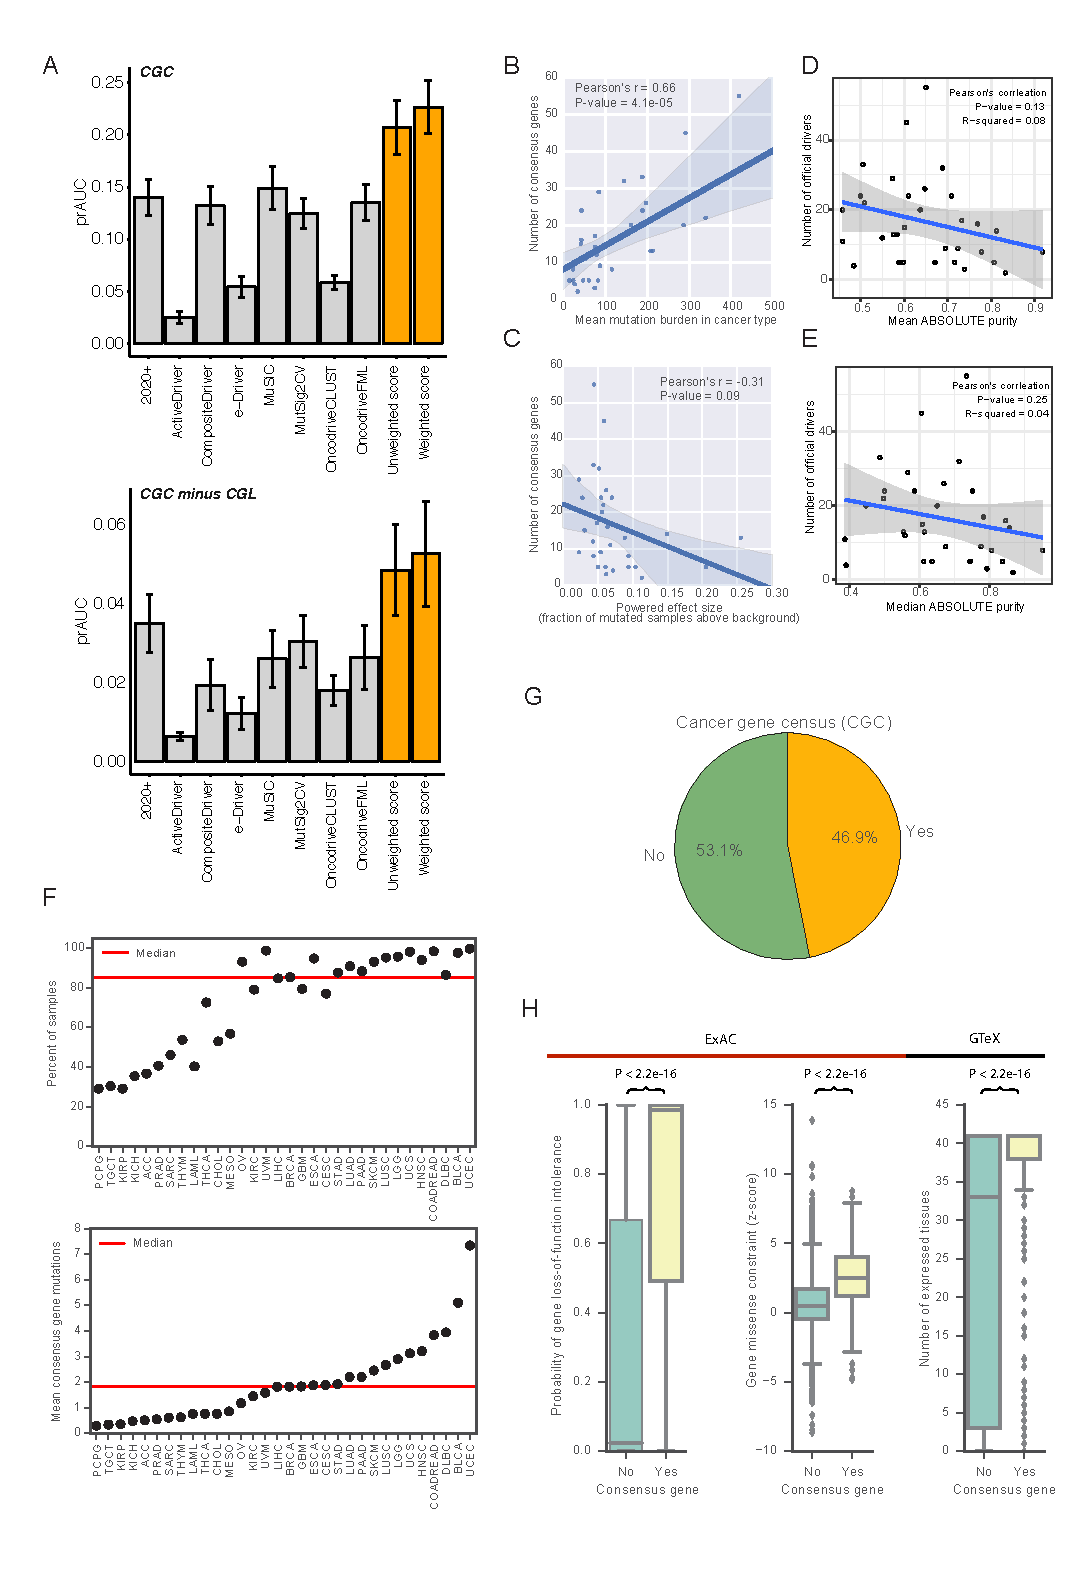
\includegraphics[width=0.9\linewidth]{figures/chapter7/analysis_of_cancer_driver_genes.pdf}
  \caption[Characteristics of consensus genes.]{(Caption next page.)}
  \label{fig:gene_characteristics}
\end{figure}
\addtocounter{figure}{-1}
\begin{figure} [t!]
\caption[(continued) Characteristics of consensus genes.]{(Figure previous page) Characteristics of consensus genes. (A) Predictive power of each individual driver gene detection method (in gray) and of the weighted and weighted scores (in orange). The predictive power was measured as prAUC, using all the genes in the Cancer Gene Census and a set that additionally excludes Cancer Genome Landscape genes used in outlier detection. Error bars, calculated by bootstrapping, indicate one standard deviation. (B) The number of consensus genes in each cancer type positively correlated with the average mutation burden. Shaded area indicates 95\% bootstrapped confidence interval. (C) Given the variability in powered effect size (fraction of mutated samples above background with 90\% power) in this study, there is a negative but not significant correlation with the number of consensus genes in each cancer type. COAD and READ were excluded because analysis was performed separately, but the final consensus genes were merged. (D) Pearson correlation between the number driver genes identified and median purity was calculated and plotted. (E) Pearson correlation between the number driver genes identified and mean purity was calculated and plotted. Summary statistics for p-value and r-squared value are reported in the top right corner of panels D and E. (F) Percent of samples containing a non-silent mutation stratified by cancer type. The red line indicates the median across cancer types (left) and average number of non-silent mutations in consensus genes per sample (right). (G) A pie chart showing the percent of consensus genes which are found in the Cancer Gene Census with annotations for small somatic mutations (missense, splice site, indel, and nonsense) (H) Consensus genes showed a higher probability for loss-of-function intolerance and missense mutation constraint of germline mutations based on ExAC, and were expressed (RPKM$>$1) in a wider number of tissues from GTeX (version 6). Given the high correlation of gene expression in the 11 brain regions assessed from GTEx, we took the median of multiple brain tissues, as done in Lek et al., 2016.}
\end{figure}

To maximize the coverage of our analysis and ensure the accuracy of our final list, previous findings were reviewed in 31 individual cancer types and PanCancer-12 from TCGA. For cancer types not yet having a TCGA publication, the relevant analysis working groups were consulted (LIHC, TGCT, UVM, SARC, PAAD, and THYM). I included in our final consensus list all those genes that were previously described as drivers by experts in the cancer-specific analysis of TCGA datasets and were also identified by at least one of the eight algorithms, even if they did not meet our consensus score threshold ($\geq$1.5)(\autoref{fig:gene_discovery}A). This resulted in an additional 54 gene-cancer pairs, such as ATR, CHEK2, IDH2, and ERCC2 in the PanCancer dataset and FOXA1 in BLCA, HRAS in SKCM, and MET in LUAD (\autoref{fig:driver_gene_approach}B-F). The majority of this effort resulted in linking cancer genes identified by our strategy to additional cancer types based on previous literature (32/54).  

\begin{figure}
  \centering
  \makeatletter
  \let\@currsize\normalsize
  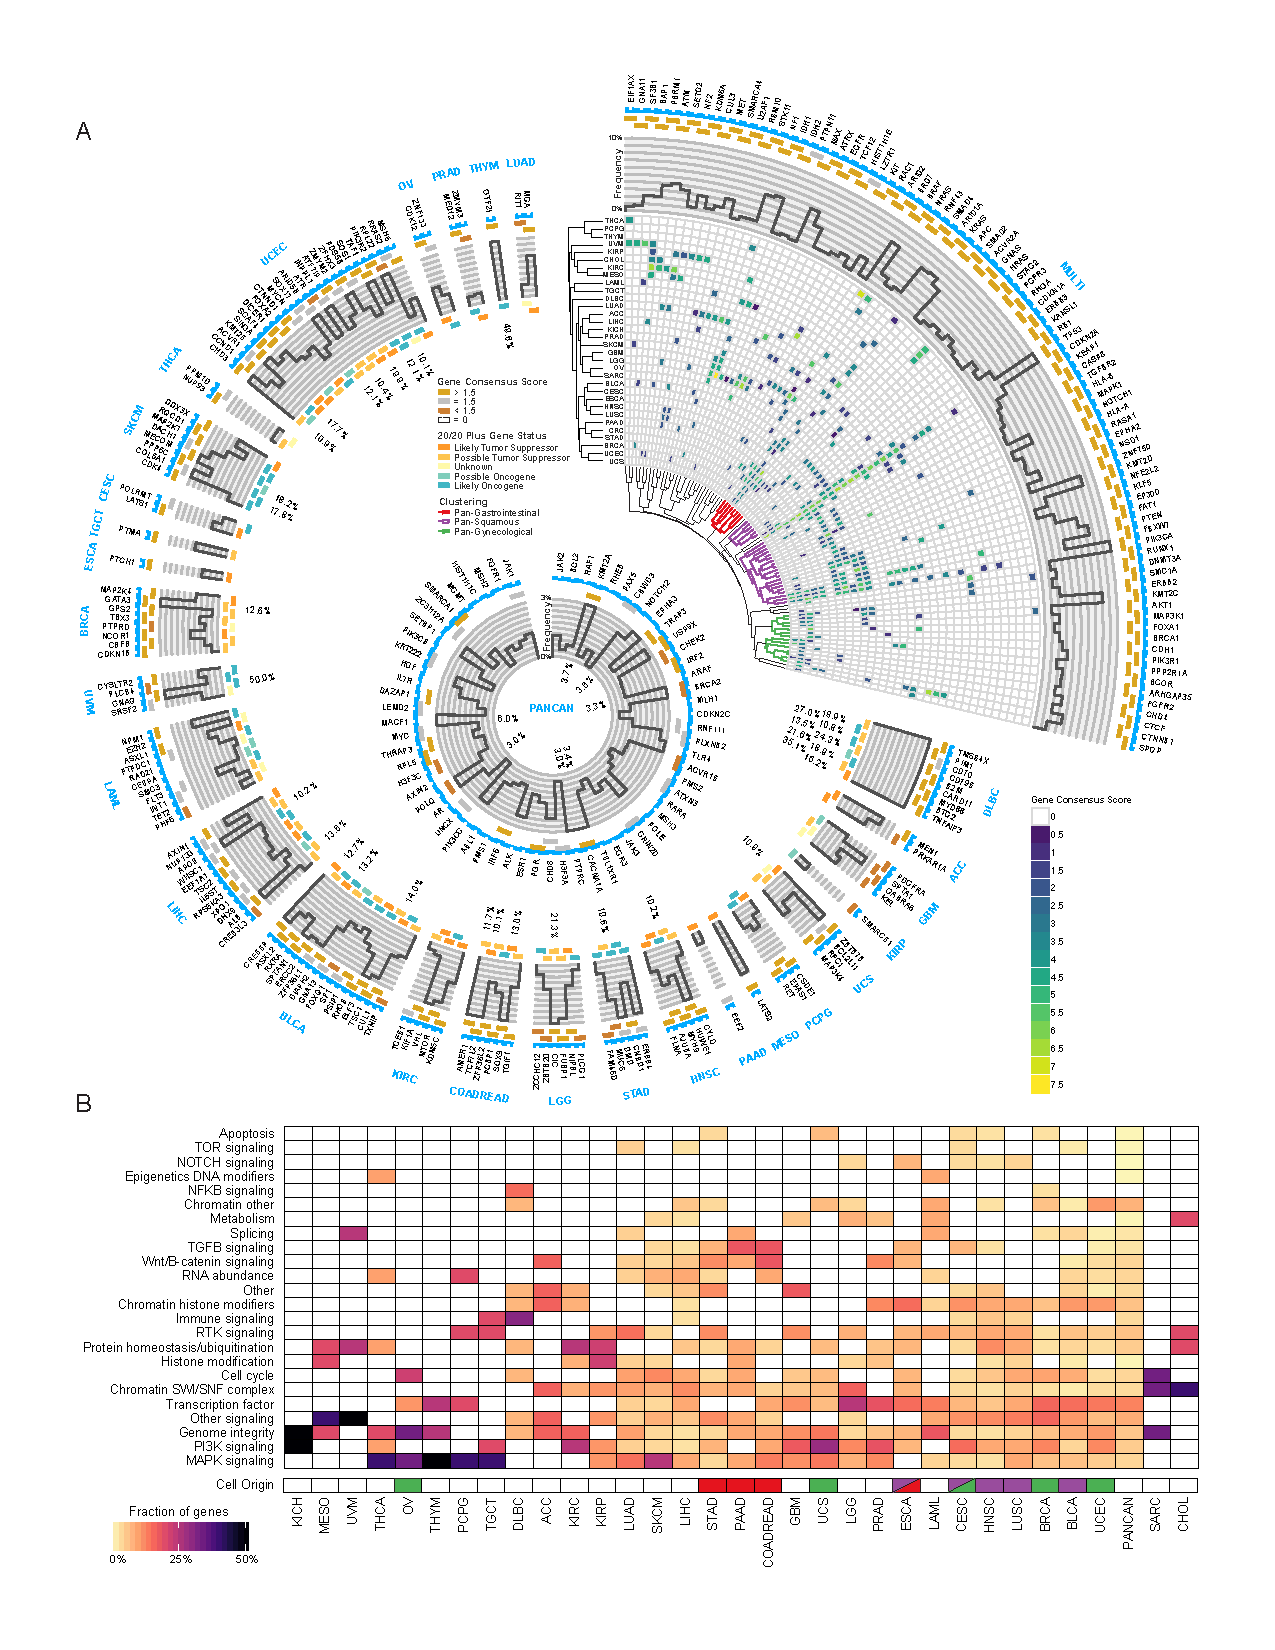
\includegraphics[width=\linewidth]{figures/chapter7/cancer_driver_genes.pdf}
  \caption[Cancer driver gene discovery]{(Caption next page.)}
  \label{fig:gene_discovery}
\end{figure}
\addtocounter{figure}{-1}
\begin{figure} [t!]
  \caption[(continued) Cancer driver gene discovery]{(Figure previous page) Cancer driver gene discovery: (A) Circos \cite{RN182} plot displays 299 cancer genes. Each sector indicates a unique cancer type (text in blue) with predicted drivers unique to that cancer type listed (gene name in black). Only tissues with at least one unique driver gene are shown. The top right sector shows all genes found significant in multiple cancer types. Next, a categorical score of gold, silver, or bronze is assigned to each gene based on the highest consensus score. If a gene was not scored and required rescue then the field is empty. The next ring illustrates the mutation frequency of a gene in our dataset. For the top right wedge, the PanCancer frequency is used, while cancer-type-specific frequencies are used in the remaining sectors. Where frequencies exceed the y-axis limit of 10\%, the innermost label indicates the frequency. The final ring uses a 5-point scale from orange to teal to represent each gene from likely tumor suppressor to likely oncogene, respectively, by the 20/20+ algorithm. Finally, in the top right slice we show hierarchical clustering of the gene consensus scores for genes that were found in more than one cancer type (note: CRC refers to the COADREAD cancer type). Additionally, significant gene clusters (permutation test) identified Pan-Gastrointestinal (red), Pan-Squamous (purple), and Pan-Gynecological tissues (green). The middle ring illustrates all genes that were only found using PanCancer results, or were otherwise rescued. (B) Heatmap showing clustering of different cancer types by pathway / biological process affected by associated consensus driver genes. Cell of origin for pan-gynecological, pan-gastrointestinal, and pan-squamous are colored as above.}
\end{figure}

To limit false positives in the expanded list, linear discriminant analysis was applied (\autoref{fig:driver_gene_approach}C). 45 genes were identified and removed from the consensus as they are likely false positives. These included CACNA1E in PanCancer, COL11A1 in LUAD, DST in GBM, and TTN in SKCM. The consensus list from the above systematic approach consisted of 258 unique genes. The average number of non-silent mutations per sample in our consensus gene list varied substantially by cancer type ranging from <1 in 12 cancer types (ACC, CHOL, KICH, KIRP, LAML, MESO, PCPG, PRAD, SARC, TGCT, THCA, and THYM) to 7.3 in UCEC. A median of 85\% of tumors harbored non-silent mutations in consensus genes across cancer types (\autoref{fig:gene_characteristics}F). 

Given the limitations of a systematic approach, 41 genes were manually rescued. In the rescue attempt, I started with a list of genes identified from previous TCGA marker papers but not found from our systematic approach. Genes were rescued with supportive evidence from the following sources: hypermutator phenotype related genes (since we excluded hypermutated samples in our systematic discovery; 6 genes), established cancer genes from LAML because of low quality variant calling originating from liquid tumor contamination of the normal samples (6 genes), genes supported by omic network tools (DriverNet and OncoIMPACT; 25 genes), and a gene supported by all three approaches from the driver mutation discovery (1 gene). Addition of genes to the final list was subjected to expert manual curation (3 genes). 

The final consensus gene list consisted of 299 unique genes across 33 cancer types and the PanCancer dataset (\autoref{fig:gene_discovery}A). The list captures most previously described driver genes for the majority of cancer types. I overlapped the cancer driver genes obtained from the consensus approach without manual curation with those from 5 independent studies in 4 cancer types (BRCA, PRAD, PAAD, and LIHC) of which one is whole-genome sequencing. The consensus approach always had a greater inter-study overlap, with an average increase of 26\% over only using a single tool, either MuSiC2 or MutSig2CV \cite{RN57, RN176, RN175, RN172, RN173, RN174}. Among the 299 genes, 59 novel genes were not previously identified in 6 previous PanCancer publications \cite{RN57, RN14, RN178, RN25, RN96, RN177, RN1} or the cancer gene census list (\url{http://cancer.sanger.ac.uk/census/})\cite{RN97}.

\subsection{Weighting strategy}
\label{sec:weighting}
Tools predicting cancer genes were weighted according to their performance in each cancer type, receiving half the weight if a result was deemed an outlier, thereby obligating additional tool agreement. Specifically, I examined quality metrics across tools and within the same tool, which allowed us to identify outlier results. I marked outliers based on the quasi-majority of three criteria: low concordance with known cancer genes, high divergence of p-value distribution from theoretical expectation, and abnormally high number of significant genes. The first criterion evaluated the fraction overlap of significant genes with a previously manually curated set of driver genes from \cite{RN25} compared with the median across all tools. The second criterion examined whether the divergence of observed p-values from those theoretically expected by the Mean Log Fold Change (MLFC) \cite{RN70} was greater than the median of all tools, which may indicate a tool's statistical assumptions may not be well satisfied. The third criterion examined whether a tool's prediction for particular cancer types appeared as an outlier in terms of the number of significant genes compared against all of the results for that tool (Tukey's outlier criterion: number significant $>$ 3Q + 1.5*IQR). I calculated a gene consensus score by summing the tools that declared the gene as being significant, with a weight of 1 for non-outlier results and 0.5 for outlier results.

\section{The landscape of cancer driver genes}

The final consensus list consists of 299 unique genes: 258 genes obtained from a systematic approach and 41 additional genes recovered after manual curation of previous TCGA marker papers with the majority (26 out of 41, 63\%) supported by additional -omic network tools (DriverNet and OncoIMPACT) not used in original SMG detection. Note that, for the rest of the analyses presented here, I will focus on the 258 genes set, but I acknowledge the limitations of a systematic approach by including the 41 genes rescued by manual curation in our final list to achieve comprehensiveness.

The list recovers most of the previously described driver genes for the majority of cancer types. In fact, in 20 out the 31 cancer types included in our study that had either been previously published or for which I had an internal list of known cancer driver genes, the recovery rate is 80\% or higher (\autoref{fig:driver_gene_approach}D and \autoref{fig:driver_gene_approach}E). The most significant outliers are STAD and the previous PanCancer study, for which I only recovered around 70\% of the previously described genes (\autoref{fig:driver_gene_approach}D). The consensus list also includes 59 novel genes that had not been described previously and other known drivers not previously associated with a given tissue. Predictions of known cancer driver genes in new tissues include ATRX in ACC, KMT2C, CTNNB1 and PTEN in BLCA, and ARID1A and KRAS in BRCA. Entirely novel predictions include GNA13 in BLCA (a homologue of the known drivers GNAQ and GNA11), RRAS2 in UCEC (with shared homology in KRAS and HRAS), and KIF1A in HNSC (a kinesin of the same family of the cancer driver KIF5B). 

The number of detected cancer driver genes varies among cancer types, with KICH having the fewest (2 genes) and UCEC having the most (55 genes). Furthermore, the ratio of predicted tumor suppressor genes and oncogenes vary widely by tissue (\autoref{fig:og_tsg_balance}). I observed a significant positive correlation (Pearson R=0.66, P value=4.1e-5) between the average mutation burden in a cancer type and the number of identified consensus genes (\autoref{fig:gene_characteristics}B). Study-based calculations for powered effect size in each cancer type did not entirely explain this phenomenon (Pearson R=-0.31, P value=0.09) (\autoref{fig:gene_characteristics}C). Regarding the associations of driver genes with different cancer types, many genes (142 out of 258) are associated with a single cancer, whereas 87 genes have driver roles in two or more cancer types, with an additional 29 genes uniquely identified using all samples combined-PanCancer approaches. As expected, TP53 is the most extreme case, as it is associated with 27 cancer types, followed by PIK3CA, KRAS, PTEN and ARID1A, each of which is associated with 15 or more tissue types (\autoref{fig:gene_discovery}A).

\begin{figure}
  \centering
  \makeatletter
  \let\@currsize\normalsize
  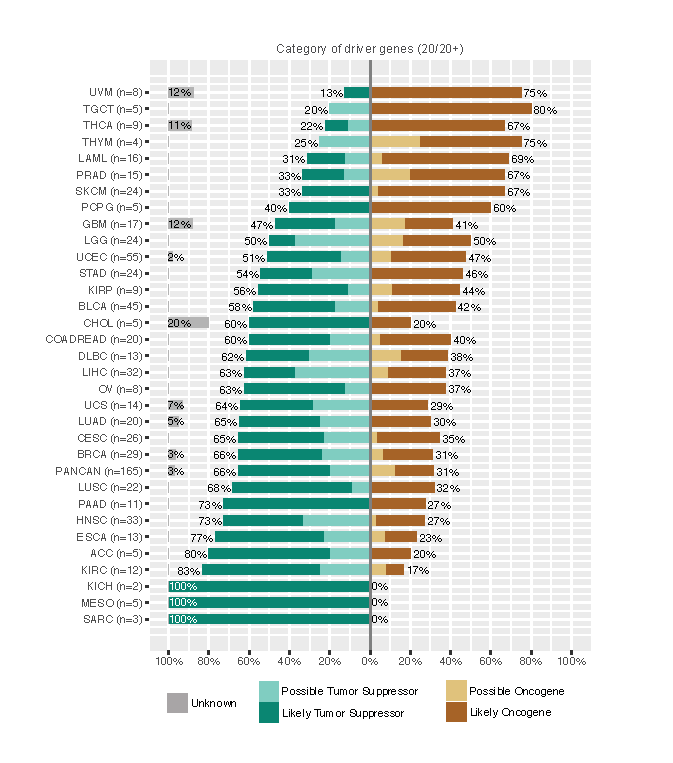
\includegraphics[width=0.9\linewidth]{figures/chapter7/og_tsg_balance.pdf}
  \caption[Balance of oncogenes and tumor suppressor genes.]{Balance of oncogenes and tumor suppressor genes. Percentage of consensus genes predicted as either oncogene (brown), tumor suppressor gene (green), or unknown (gray) by the 20/20+ algorithm, an improved version of the 20/20 rule. The 20/20+ algorithm uses a supervised-learning approach (random forests) and bases predictions on the mutational patterns observed within a gene. \q{Likely} and \q{Possible} statuses were determined at a threshold of 0.05 for q-value (Benjamini-Hochberg method) and p-value, respectively. Consensus genes were designated as \q{Unknown} if they did not meet these thresholds. N represents the number of significant genes in each cancer type.}
  \label{fig:og_tsg_balance}
\end{figure}

I clustered the different cancer types according to the consensus scores of their associated genes. Remarkably, some cancer types grouped according to their tissue of origin, such as LGG and GBM; while others according to their cell of origin. The most significant of the cell origin clusters spans all the squamous cancer types (BLCA, CESC, ESCA, HNSC and LUSC, (permutation test, adjusted p $<$ 0.01) and includes several transcription factors (ZNF750, NFE2L2 or KLF5), chromatin and histone modifiers (KMT2D, EP300, or NSD1), and various PI3K pathway genes (PIK3CA, PTEN or MAPK1). I found two additional significant clusters (permutation test, adjusted p $<$ 0.05) that group gynecological (UCS, CESC, UCEC, OV, and BRCA) as well as gastrointestinal cancers (COADREAD, PAAD, ESCA and STAD) (\autoref{fig:gene_discovery}A). 

Finally, I classified the consensus driver genes according to the cancer-related biological processes and pathways with which they were associated (\autoref{fig:gene_discovery}B). For most genes, the categories (excluding \q{other} and \q{other signaling}) clearly reflect known processes involved in carcinogenesis, as they are \q{transcription factor} (39 genes), \q{RTK signaling} (16) and \q{RNA abundance} (15), \q{protein homeostasis/ubiquitination} (15), \q{chromatin histone modifiers} (15), \q{genome integrity} (14), \q{chromatin other} (14) and, remarkably, \q{immune signaling} (10). The last group is of particular interest, given the connection between driver genes and immune response. In terms of cancer types, most have at least one cancer driver that belongs to either genome integrity (28 out of 33 cancer types) or the MAPK or PI3K signaling pathways (24 and 22 cancer types, respectively). Interestingly, the squamous cancer types were again grouped together when looking at which processes and pathways associated with their driver genes, having higher proportions of genes involved in chromatin histone modification as well as receptor-tyrosine kinase and immune signaling. 

\section{Driver mutation approach}

To maximize the coverage of our analysis I used 12 tools that look for three distinct hallmarks of \q{driverness}.  The collection was comprised of 8 mutation-level algorithms (SIFT \cite{RN9}, PolyPhen2 \cite{RN10}, MutationAssessor \cite{RN38}, transFIC \cite{RN53}, fathmm \cite{RN39}, CHASM \cite{RN29}, CanDrA \cite{RN36} and VEST \cite{RN30}), and 4 structure-based (HotSpot3D \cite{RN132}, HotMAPS \cite{RN60}, 3DHotSpots.org \cite{RN133} and e-Driver3D \cite{RN45}). In order to combine the predictions from the sequence-based approaches I used principal component analysis to develop a Combined Tool Adjusted Total (CTAT) scores for both, population-based and cancer-specific scores. Principal component analysis has been previously shown successful in a similar task of prioritizing germline mutations \cite{RN179}. I also combined the results from three-dimensional tools by adding the number of tools that predicted a specific position as belonging to a cancer-mutation cluster. Finally, to limit the number of false positives, I focused our analysis on the genes of our consensus driver list.

The CTAT score combines multiple individual tools that prioritize missense mutations. To normalize each score, I calculated the z-score by subtracting the mean score and then dividing by the standard deviation. I then performed principal component analysis (PCA) using ScikitLearn v0.18.0 and used the score along the first principal component as our CTAT score, representing the scalar projection onto the first eigenvector. Only missense mutations that had no missing values for each of the combined tools were used in generating the principal component analysis. I performed this procedure on two distinct categories of tools, \q{population-based} tools that distinguish damaging/pathogenic germline missense variants from common polymorphisms (SIFT, PolyPhen2, VEST, and MutationAssessor), and \q{cancer-focused} tools designed to distinguish somatic missense mutations that are drivers from passengers (CHASM, CanDrA, fathmm, and transFIC). To score the remaining missense mutations that did have a missing score, I imputed missing scores of the individual tool with the mean for the method. Imputation was only performed for the cancer-focused tools as the population-based tools had too many missing values.

To define the CTAT score thresholds, I used the maximum balanced accuracy when predicting OncoKB mutations \q{oncogenic} or \q{likely oncogenic}. This yielded a threshold of 1.2 for CTAT-population and 2.4 for CTAT-cancer. For the structural algorithms, I report a mutation as likely driver if at least 2 algorithms identify it within a cluster. Finally, I evaluated the performance of each CTAT score using mutations from OncoKB labeled as \q{likely oncogenic} or \q{oncogenic} as true-positives. 

\section{Discovery of driver mutations}

Not all mutations in a cancer driver gene have the same impact on its function \cite{RN183}. Their consequences frequently depend on which position within the protein is affected and what amino acid change is induced \cite{RN29}. Here, I sought to explore this topic across the entire PanCancer dataset, classifying 751,876 unique missense mutations by examining the 299 cancer driver genes that I identified, according to their predicted oncogenic effect. I combined the output of three different categories of tools into consensuses approaches: (I) tools that distinguish between benign and pathogenic mutations using sequence-based features (CTAT-population); (II) tools that distinguish between driver and passenger mutations using sequence-based features (CTAT-cancer); and (III) tools that discover statistically significant three-dimensional clusters of missense mutations (Structure-based); these identified 10,098 (1.3\% of the total missense mutations), 4,595 (0.6\%), and 1,469 (0.2\%) unique amino acid substitutions, respectively (\autoref{fig:driver_mutation}A). The differences in the number of predicted driver mutations for each approach are likely due to the design and requirements of the tools, i.e., dependence of structural clustering tools on available three-dimensional protein structures (either experimental or homology-based) yields fewer predicted driver mutations. Nevertheless, structural tools may provide additional molecular biological context for the identified mutations, which can be particularly relevant for variants of unknown significance (VUS) \cite{RN184}.

\begin{figure}
  \centering
  \makeatletter
  \let\@currsize\normalsize
  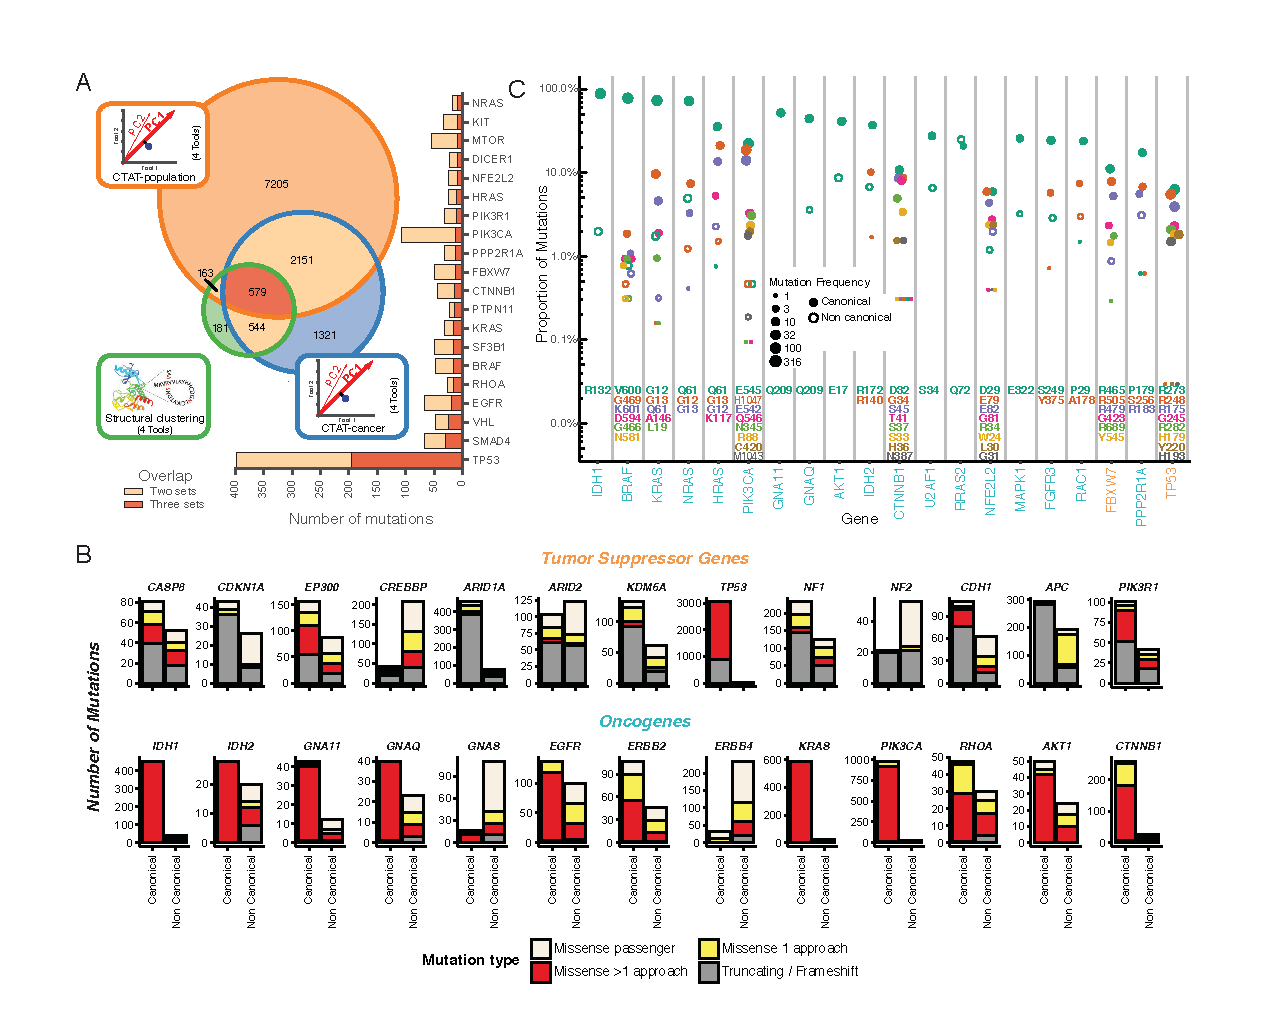
\includegraphics[width=\linewidth]{figures/chapter7/driver_mutation.pdf}
  \caption[Driver mutation discovery approaches, overview, overlap, and contrasts]{Driver mutation discovery approaches, overview, overlap, and contrasts: (A) Venn diagram indicates total number of mutations overlapping among three consensus approaches-CTAT-population, CTAT-cancer, and structural clustering. Adjacent bar chart indicates the top 20 genes sorted by 3-set intersecting mutation counts. (B) Driver gene discovery identified gene-tissue pairs (canonical genes) in tumor suppressors and oncogenes. However, some gene-tissue pairs were not identified in driver discovery (non-canonical). Mutation frequency from canonical and non-canonical cancer genes are displayed and divided among 4 mutation classes: truncation/frameshift mutations (grey); missense mutations uniquely identified by only one approach (yellow, see Panel A); missense mutations identified by multiple approaches (red, see Panel A); and missense passenger mutations not identified by any approach (off white). (C) Mutation percentage out of all missense and truncating/frameshift mutations within a gene is shown on the y-axis (log scale). Point size is log scaled and represents amino acid position frequency. The top 23 genes ordered by increasing mutational diversity (normalized entropy) and only the 9 most frequently mutated amino acid positions for each gene are shown.}
  \label{fig:driver_mutation}
\end{figure}

When benchmarked against OncoKB \cite{RN144}-a manually curated dataset of cancer mutations annotated according to likely oncogenic effect, cancer-focused algorithms had higher predictive value than algorithms that distinguished between benign and pathogenic mutations. In addition, the CTAT-cancer score outperformed all individual sequence-based approaches. 

Overall, there are 9,919 predicted cancer driver mutations in our cohort (3,437 unique mutations) identified by 2 or more approaches from CTAT-population, CTAT-cancer, or structural clustering. These mutations affect 5,782 tumor samples. I observed that these missense driver mutations represent a greater fraction of the total mutations in oncogenes than in tumor suppressors (\autoref{fig:driver_mutation}B). In this latter group, most mutations seem to be truncating or frameshift, a result in agreement with previous observations \cite{RN185}. Nevertheless, there are also tumor suppressor genes having high numbers of missense driver mutations, such as EP300, CREBBP, CASP8, PIK3R1 and TP53 (Figure 7.5B). An interesting example is CDH1, which is mostly affected by truncating or frameshift mutations in BRCA (75 out of 85 mutations), but mostly targeted by missense driver mutations in STAD (21 out of 25 mutations). This could suggest different roles for CDH1 in these two cancer types.

I was also intrigued by missense driver mutations detected in cancer types where the gene was not predicted to be a driver. This subset is particularly important for genotype-driven clinical trials \cite{RN186}. Overall, there are 1,719 of tissue-unmatched likely driver mutations (19\% of the total) in 1,431 patients (16\%) and there are 502 patients whose only predicted missense driver mutations affect genes not yet known to play a role in that cancer type. For example, I identified 28 patients with predicted EGFR driver mutations in cancer types where EGFR is not yet identified as a common driver gene, such as HNSC, STAD, LUSC, UCEC, ESCA and LIHC. In some extreme cases, such as ERBB4 or GNAS, these mutations actually represent the majority of predicted driver missense mutations in the gene (\autoref{fig:driver_mutation}B). Additionally, 2\% (10/457) of IDH1 missense events that occur at the amino acid position R132 are found in tissues not typically known to carry such mutations i.e. BLCA (n=2), BRCA (2), COADREAD (2), LUAD (2), PCPG (1), and THYM (1) (\autoref{fig:driver_mutation}C). Furthermore, I observed that RRAS2 Q72, a predicted oncogene in UCEC (n=5 samples) with strong homology to KRAS Q61 and HRAS Q61, was also mutated in cancer types in which it was not predicted to be an oncogene - UCS (n=1), LUSC (1), LUAD (1), PRAD (1), HNSC (1), and TCGT (1). Any analysis focusing only on common driver genes and mutations known in that cancer type would very likely miss presumed driver mutations for those patients. These results emphasize the advantage of PanCancer panels of driver mutations in order to maximize the coverage of driver-detection analyses.

\section{Value of structure-based analysis}

Results were compared to an independent dataset of 1,049 experimentally tested somatic mutations to validate our driver mutation predictions \cite{RN187}. Briefly, SNVs were introduced to two cancer cell lines, Ba/F3 and MCF10A, and were evaluated for their oncogenicity based on survival and growth. In total, 160 mutations from 19 genes were validated in this dataset. The percentage of functionally validated mutations increased from 60\% predicted with CTAT-population, to 61\% for those found by CTAT-cancer, and 78\% for Structure-based analysis (\autoref{fig:driver_mutation_examples}A). Among the 579 mutations predicted by all three approaches, 39 of the 46 that were tested (85\%) were also validated. Further, the sensitivity and specificity of identifying driver mutations annotated by OncoKB suggests performance is generalizable to a larger set of genes. These results support the value of the prediction algorithms used in our study and the advantage of combining multiple tools. Also, I would like to note that this approach only addresses true positive findings and represents a floor estimate for computational predictions.

\begin{figure}
  \centering
  \makeatletter
  \let\@currsize\normalsize
  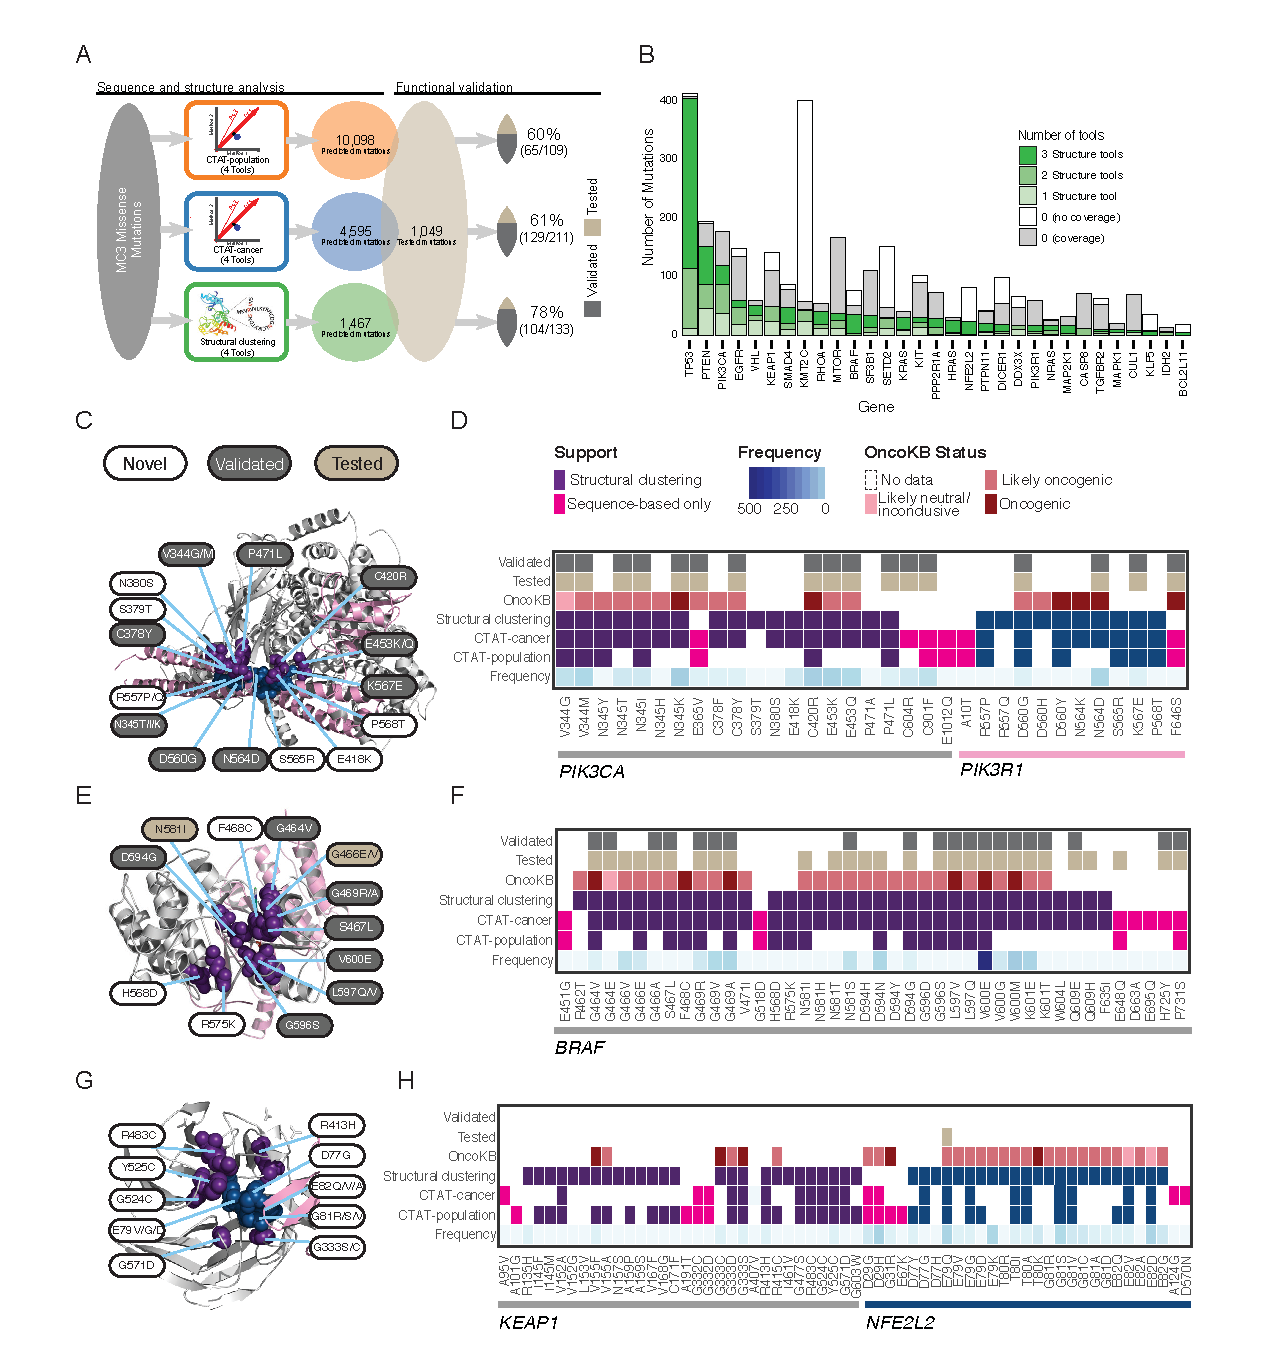
\includegraphics[width=\linewidth]{figures/chapter7/driver_mutation_examples.pdf}
  \caption[Driver mutation discovery and validation]{(Caption next page.)}
  \label{fig:driver_mutation_examples}
\end{figure}
\addtocounter{figure}{-1}
\begin{figure} [t!]
  \caption[(continued) Driver mutation discovery and validation]{(Figure: previous page) Driver mutation discovery and validation: (A) This schematic displays the steps taken to assess consensus among mutation-level predictions using sequence-based and structural clustering tools and comparing them to an orthogonal set of functionally validated mutations. From left to right: the grey box represents the missense mutations that were processed by 12 tools from 3 categories (population-based, cancer-focused, and structural clustering tools) and combined into three consensus approaches (CTAT-population, CTAT-cancer, and structural clustering). Finally, the total number and percentage of functionally validated/tested mutations is shown. (B) The number of mutations (y-axis) found by structural tools for each gene (x-axis) are shaded according to support by structural tools (green). Those mutations without support are distinguished by two categories, with (grey) and without (white) available protein structure.  Heatmaps (D, F, H) coupled with protein structure (C, E, G) are shown in panels for the proteins PIK3CA/PIK3R1 (PDB ID: 4OVU), BRAF (4MBJ), and KEAP1/NFE2L2 (3ZGC), respectively, and display whether a particular mutation was detected by sequence-based (CTAT-population or CTAT-cancer) or structure-based approaches (at least two structural tools). Purple/teal colors distinguish proteins (PIK3CA/PIK3R1 and KEAP1/NFE2L2 pairs) for mutations found by structure-based approaches, while pink boxes indicate mutations found only by sequence-based approach. Additionally, for each mutation, frequency (blue gradient), OncoKB status (red gradient), testing status (tan), and validation status (grey) are provided. All mutations found by structure-based approaches in each of the 3 genes are shown with a few additional mutations that are only found by sequence-based approaches. Key mutations are highlighted from the heatmaps and labeled with white, grey, and tan labels referring to novel, validated, and tested (not validated) mutations, respectively.}
\end{figure}

Structural-based mutations clustered on 66 proteins, including one cluster on KLF5, a gene not previously identified in PanCancer studies and ranked among the top 30 clusters by PanCancer mutation frequency (\autoref{fig:driver_mutation_examples}B). I sought to examine in more detail the predictions of the three approaches in various well-established cancer driver genes, such as PIK3CA/PIK3R1, BRAF, and KEAP1/NFE2L2 (\autoref{fig:driver_mutation_examples}C-4H). The interface between PIK3CA and PIK3R1 contains a cluster of mutations that were found by at least 2 of the approaches and includes both mutations that were validated and those not tested. D560G, N564D, and K567E are validated mutations that cluster closely to non-tested mutations R577P/Q, S565R, and P568T in PIK3R1. Similarly, PIK3CA contains validated mutations C378Y, V344G/M, N345T/I/K, P471L, C420R, and E418K clustering with non-tested mutations S379T, N380S, and E418K. These non-tested mutations are excellent candidates for further experimental validation due to their close proximity to known validated driver mutations as well as support from sequence-based approaches (\autoref{fig:driver_mutation_examples}C and \ref{fig:driver_mutation_examples}D). BRAF also contains clusters similar to this PIK3CA/PIK3R1 cluster, with a mixture of validated and novel mutations (\autoref{fig:driver_mutation_examples}E and \autoref{fig:driver_mutation_examples}F). 

Additionally, there are many genes that contain mutations found by all three approaches but that were not tested experimentally, including KEAP1, NFE2L2, RHOA, MTOR, MAP2K1, and VHL. Nevertheless, many of these driver mutations have orthogonal evidence from OncoKB. For example, the mutations G333D/S in KEAP1 have an OncoKB status of likely oncogenic and oncogenic, respectively (\autoref{fig:driver_mutation_examples}G and \ref{fig:driver_mutation_examples}H). There are also NFE2L2 mutations that cluster closely with the KEAP1 mutations along the protein-protein interface (D77, E82, G81, E79) and were not experimentally validated but have an OncoKB status of either likely-oncogenic or oncogenic. Other KEAP1 mutations in the same cluster found by all three approaches are R483C, Y525C, G524C, G571D, and R413H. However, none of these mutations were tested in our dataset, nor have evidence from OncoKB. Given their proximity to the validated KEAP1 sites and the bioinformatic evidence that I found, these mutations are ideal candidates for follow-up validation experiments. 

Overall, this analysis reinforces the notion that sequence-based approaches and structure-based approaches ought to be used in conjunction and tend to be complementary. For example, E365V, C604R, and C901F in PIK3CA, F646S in PIK3R1, and H725Y and P731S in BRAF were found by sequence-based approaches but not the structure-based approach and are experimentally validated (Figures \ref{fig:driver_mutation_examples}D and \ref{fig:driver_mutation_examples}F). Conversely, R462T in BRAF was only found through a structural approach and not sequence-based approaches and is annotated as likely oncogenic in OncoKB (Figures \ref{fig:driver_mutation_examples}F and \ref{fig:driver_mutation_examples}H). Finally, I note that, while looking at mutations detected by all 3 approaches provides high confident driver mutations, there may still be important driver mutations that were missed. 

\section{Conclusions}
%!TEX root = root.tex

\chapter{Concluding remarks}
\label{chap:ch8}
\chaptermark{Concluding remarks}

The first confirmed human cancer driver gene, HRAS, was identified in 1982. In just the past decade, the list of likely cancer driver genes has rapidly grown. Although partly reflecting the growth in size of studies due to advances in next generation sequencing, it also reflects improvements in computational techniques. Computational methods are starting to become more robust with realistic models of how somatic mutations accumulate in cancer. Moreover, studies are now moving to understanding cancer drivers at increasing resolution -- moving from genes to individual mutations.

The first part of my dissertation (Chapter 2) focuses on how to appropriately statistically model the accumulation of somatic mutations in cancer. The typical choice of modeling the background mutation rate is problematic because it is highly variable at multiple scales. However, a key insight is covariates modulate mutation rate at the scale of megabases within the genome, but nearly all genes span $<$1MB. By statistically conditioning on the total number of mutations within a gene when simulating mutations, nuisance factors influencing mutation rate that are not always measured or known are substantially lessened. This approach allows substantial flexibility in comprehensively modeling many mutational patterns indicative of positive selection in cancer.

Here, I propose several new computational methods to analyze cancer drivers at different levels -- such as the gene (20/20+, Chapter 3), region (HotMAPS, Chapter 5), and mutation (CHASMplus, Chapter 6). I used these methods to interrogate fundamental questions regarding cancer driver mutations, such as their cancer type specificity, commonness or rarity, the balance and characteristics of oncogenes and tumor suppressor genes, and the likely future trajectory of cancer driver discovery. Due to the lack of a gold-standard for cancer drivers, I also developed a benchmark for cancer driver gene prediction (Chapter 4).




Although the landscape of cancer drivers in primary cancers are progressively getting more fully explored, there remains many aspects that are still poorly understood. Sequencing untreated primary cancers gives an understanding of one time point in the natural evolutionary history of cancers. Understanding the full heterogeneity and dynamics of cancer will require sequencing both before (pre-cancerous lesions) and after (metastases). This will provide more understanding of such questions as: are there major metastasis-drivers?, and how much does the temporal ordering of driver mutations matter as opposed to overall driver mutation burden?

A complete catalog of all cancer drivers, in it of it self, will not suffice. Cancer driver mutations will need to be related to their functional consequence and interaction with the microenvironment and other driver mutations. A mechanistic insight may be critical for a rational understanding of the effects of targeted drugs and optimization of drug combinations.



\appendix
%!TEX root = root.tex
\appendix

\begingroup             
\let\clearpage\relax

%\chapter{Glossary of Terms}
%\label{app:glossary}

\newglossaryentry{cancer driver mutation}{name={cancer driver mutation},description={A mutation that increases the net growth advantage of a cancer cell* under the specific microenvironmental context encounter \textit{in vivo} in humans. *=cancer driver mutations may occur prior to a cell clone officially becoming cancer and has the theoretical possibility that the mutation is no longer advantageous for the cancer cell at a later time. However, a cancer driver mutation should be advantageous at least at certain parts towards the development or progression of cancer}}

\newglossaryentry{microenvironment}{name={microenvironment},description={The local environment surrounding and within the tumor}}

\newglossaryentry{driver mutation}{name={driver mutation},description={Shorthand for cancer driver mutation}}

\newglossaryentry{cancer driver gene}{name={cancer driver gene},plural={cancer driver genes},description={A gene that contains at least one cancer driver mutation}}

\newglossaryentry{cancer drivers}{name={cancer drivers },description={A genetic loci that contains driver mutations, without reference specifically to whether it is a gene, region, or a mutation}}

\newglossaryentry{intra-tumor heterogeneity}{name={intra-tumor heterogeneity},description={Heterogeneity among cells within a tumor. Here, specifically referring to different usage of cancer driver mutations}}

\newglossaryentry{OG}{name={OG},description={oncogene}}

\newglossaryentry{TSG}{name={TSG},description={tumor suppressor gene}}

\newglossaryentry{somatic mutation}{name={somatic mutation},description={starting from embryogenesis, mutations that occur in the cells of the body (excluding germ cells), and therefore are not inherited}}

\newglossaryentry{random forest}{name={random forest},description={A supervised machine learning algorithm consisting of an ensemble of randomized decision trees}}

\newglossaryentry{decision tree}{name={decision tree},description={A decision tree is a set of questions asked recursively (in a tree-like manner) to predict either a categorical value (classification) or continuous value (regression)}}

\newglossaryentry{mutation hotspot}{name={mutation hotspot},description={A genomic or protein loci with highly localized mutations}}

%\glsaddall[]
\glsaddallunused
\printglossary
\endgroup

%% REFERENCES
% if you use BIBTEX

\bibliographystyle{IEEEtran}
\bibliography{IEEEabrv,thesis} % PLEASE USE THE APPROPRIATE BIBLIOGRAPHY STYLE FOR YOUR DISSERTATION !!!!!!!!!!!!!


%!TEX root = root.tex

\begin{vita}
\ssp

\noindent\begin{large}\textbf{Collin Tokheim}\end{large}\\
116 W University Pkwy, APT 1226 \\
Baltimore, MD, 21210 \\
ctokheim@jhu.edu \\
\vspace{5pt}
\hrule
\vspace{10pt}
\vskip .1in
%\hrulefill 

\noindent\begin{large}\textbf{EDUCATION}\end{large}
\vskip .1in
\noindent Johns Hopkins University \\
Ph.D., Biomedical Engineering, (expected may) 2018 \\
GPA 4.0/4.0 \\

\noindent University of Iowa \\
BSE, Biomedical Engineering, 2011 \\
GPA 4.0/4.0 \\

\noindent\begin{large}\textbf{RESEARCH EXPERIENCE}\end{large}
\vskip .1in
\noindent\textbf{Graduate research assistant, Johns Hopkins University (2014-2018)}\\
\textit{Advisor: Dr. Rachel Karchin, Biomedical Engineering and Oncology}\\
Topic: Statistical identification of mutational drivers in human cancers through development of cutting-edge computational methods\\

\noindent\textbf{Staff research associate, University of California, Los Angeles (1/2013-6/2013)}\\
\textit{Advisor: Dr. Yi Xing, Microbiology, Immunology, \& Molecular Genetics}\\
Topic: Genomic analysis of the transcriptome with emphasis on alternative splicing\\

\noindent\textbf{Research Assistant, University of Iowa (4/2011-12/2012)}\\
\textit{Advisor: Dr. Yi Xing, Microbiology, Immunology, \& Molecular Genetics}\\
Topic: Genomic analysis of the transcriptome with emphasis on alternative splicing\\

\noindent\textbf{Undergraduate Research Assistant, University of Iowa (4/2010-8/2011)}\\
\textit{Advisor: Dr. Xiaodong Wu, Electrical and Computer Engineering and Radiation Oncology}\\
Topic: Computational analysis of computed tomography (CT) scans of tumors.\\

\noindent\begin{large}\textbf{DISTINCTIONS, AWARDS, \& HONORS}\end{large}
\vskip .1in
\begin{itemize}
  \itemsep0em
  \item Martin and Carol Macht Award (2018)
  \item First author PNAS paper featured in Baltimore Sun newspaper (Jan 2017)
  \item National Cancer Institute (NCI) NRSA Fellowship F31CA200266 (2015-present)
  \item Alpha Eta Mu Beta Biomedical Engineering Honor Society (2016-present)
  \item Top performing team in the Personal Genome Project challenge in Critical Assessment of Genome Interpretation (CAGI) competition (Mar 2016)
  \item Graduated with Highest Distinction (May 2011)
  \item Tau Beta Pi Engineering Honor Society (2010-present) 
  \item William C. Blackburn Engineering Scholarship (2009-2011)
  \item University of Iowa President's List (2008-2011) 
  \item E. Lester and Frances M. Williams Fund Scholarship (2008-2009)
  \item College of Engineering Dean's List (2007-2011)
  \item Engineering Excellence Scholarship (2007-2008)
\end{itemize}
\vskip .15in

\noindent\begin{large}\textbf{PEER-REVIEWED PUBLICATIONS}\end{large}
\vskip .1in
\noindent(Google Scholar H-index = 7, total citations = 295)\\
* co-first author
\vskip .1in

Matthew H. Bailey*, \underline{Collin Tokheim}*, Eduard Porta-Pardo*, Sohini Sengupta, Denis Bertrand, Amila Weerasinghe, Antonio Colaprico, Michael C. Wendl, Jaegil Kim,  Brendan Reardon, Kwok-Shing Ng, Kang Jin Jeong, Song Cao, Zixing Wang, JianJiong Gao, Qingsong Gao, Fang Wang, Eric Minwei Liu, Loris Mularoni, Carlota Rubio-Perez, Niranjan Nagarajan, Isidro Cortés-Ciriano, Daniel Cui Zhou, Wen-Wei Liang, Julian M. Hess, Venkata D. Yellapantula, David Tamborero, Abel Gonzalez-Perez, Chayaporn Suphavilai, Jia Yu Ko, Ekta Khurana, Peter J. Park, Eliezer Van Allen, Han Liang, The MC Working Group, The Cancer Genome Atlas Research Network, Michael Lawrence, Adam Godzik, Nuria Lopez-Bigas, Josh Stuart, David Wheeler, Gad Getz, Ken Chen, Alexander J. Lazar, Gordon B Mills, Rachel Karchin, Li Ding. Comprehensive Discovery and Characterization of Driver Genes and Mutations in Cancer. Cell. In Press.\\

\underline{Tokheim, C. J.}, Papadopoulos, N., Kinzler, K. W., Vogelstein, B. \& Karchin, R. Evaluating the evaluation of cancer driver genes. Proc Natl Acad Sci U S A 113, 14330-14335, doi:10.1073/pnas.1616440113 (2016).\\

\underline{Tokheim, C.}, Bhattacharya, R., Niknafs, N., Gygax, D. M., Kim, R., Ryan, M., Masica, D. L. \& Karchin, R. Exome-Scale Discovery of Hotspot Mutation Regions in Human Cancer Using 3D Protein Structure. Cancer Res 76, 3719-3731, doi:10.1158/0008-5472.CAN-15-3190 (2016).\\

Bertotti, A., Papp, E., Jones, S., Adleff, V., Anagnostou, V., Lupo, B., Sausen, M., Phallen, J., Hruban, C. A., \underline{Tokheim, C.}, Niknafs, N., Nesselbush, M., Lytle, K., Sassi, F., Cottino, F., Migliardi, G., Zanella, E. R., Ribero, D., Russolillo, N., Mellano, A., Muratore, A., Paraluppi, G., Salizzoni, M., Marsoni, S., Kragh, M., Lantto, J., Cassingena, A., Li, Q. K., Karchin, R., Scharpf, R., Sartore-Bianchi, A., Siena, S., Diaz, L. A., Jr., Trusolino, L. \& Velculescu, V. E. The genomic landscape of response to EGFR blockade in colorectal cancer. Nature 526, 263-267, doi:10.1038/nature14969 (2015).\\

Patrick Kwok-Shing Ng, J. L., Kang Jin Jeong, Shan Shao, Hu Chen, Yiu Huen Tsang, Sohini Sengupta, Zixing Wang, Venkata Hemanjani Bhavana, Richard Tran, Stephanie Soewito, Darlan Conterno Minussi, Daniela Moreno, Kathleen Kong, Turgut Dogruluk, Hengyu Lu, Jianjiong Gao, \underline{Collin Tokheim}, Daniel Cui Zhou, Jia Zeng, Carman Ka Man Ip, Zhenlin Ju, Matthew Wester, Shuangxing Yu, Yongsheng Li, Christopher Vellano, Nikolaus Schultz, Rachel Karchin, Li Ding, Yiling Lu, Lydia Wai Ting Cheung, Ken Chen,  Kenna R. Shaw, Funda Meric-Bernstam, Kenneth L. Scott, Song Yi, Nidhi Sahni, Han Liang, and Gordon B. Mills. Systematic Functional Annotation of Somatic Mutations in Cancer. Cancer Cell. In press.\\

Chung, C. H., Guthrie, V. B., Masica, D. L., \underline{Tokheim, C.}, Kang, H., Richmon, J., Agrawal, N., Fakhry, C., Quon, H., Subramaniam, R. M., Zuo, Z., Seiwert, T., Chalmers, Z. R., Frampton, G. M., Ali, S. M., Yelensky, R., Stephens, P. J., Miller, V. A., Karchin, R. \& Bishop, J. A. Genomic alterations in head and neck squamous cell carcinoma determined by cancer gene-targeted sequencing. Ann Oncol 26, 1216-1223, doi:10.1093/annonc/mdv109 (2015).\\

Li Ding, M. H. B., Eduard Porta-Pardo, Vesteinn Thorsson, Antonio Colaprico, Denis Bertrand, David L. Gibbs, Amila Weerasinghe, Kuan-lin Huang, Matthew A Wyczalkowski, Sam Q. Sun, \underline{Collin Tokheim}, Reyka Jayasinghe, Feng Chen, Lihua Yu, Alison M Taylor, Andrew D Cherniack, Jaegil Kim, Rehan Akbani, Chayaporn Suphavilai, Niranjan Nagarajan, Joshua M. Stuart, Gordon B Mills, Benjamin Vincent, Carolyn M Hutter, Jean Claude Zenklusen, Katherine A Hoadley, Michael C. Wendl, llya Shmulevich, Alexander J. Lazar, David Wheeler, Gad Getz, The Cancer Genome Atlas Research Network. Perspective on Central Oncogenic Processes at the End of the Beginning of Cancer Genomics. [Submitted]\\

\underline{Tokheim, C.}, Park, J. W. \& Xing, Y. PrimerSeq: Design and visualization of RT-PCR primers for alternative splicing using RNA-seq data. Genomics Proteomics Bioinformatics 12, 105-109, doi:10.1016/j.gpb.2014.04.001 (2014).\\

Masica, D. L., Douville, C., \underline{Tokheim, C.}, Bhattacharya, R., Kim, R., Moad, K., Ryan, M. C. \& Karchin, R. CRAVAT 4: Cancer-Related Analysis of Variants Toolkit. Cancer Res 77, e35-e38, doi:10.1158/0008-5472.CAN-17-0338 (2017).\\

Park, J. W., \underline{Tokheim, C.}, Shen, S. \& Xing, Y. Identifying differential alternative splicing events from RNA sequencing data using RNASeq-MATS. Methods Mol Biol 1038, 171-179, doi:10.1007/978-1-62703-514-9\_10 (2013).\\

Wang, J., Lu, Z. X., \underline{Tokheim, C. J.}, Miller, S. E. \& Xing, Y. Species-specific exon loss in human transcriptomes. Mol Biol Evol 32, 481-494, doi:10.1093/molbev/msu317 (2015). \\

Lu, Z. X., Huang, Q., Park, J. W., Shen, S., Lin, L., \underline{Tokheim, C. J.}, Henry, M. D. \& Xing, Y. Transcriptome-wide landscape of pre-mRNA alternative splicing associated with metastatic colonization. Mol Cancer Res 13, 305-318, doi:10.1158/1541-7786.MCR-14-0366 (2015). \\

Rettig, E. M., Talbot, C. C., Jr., Sausen, M., Jones, S., Bishop, J. A., Wood, L. D., \underline{Tokheim, C.}, Niknafs, N., Karchin, R., Fertig, E. J., Wheelan, S. J., Marchionni, L., Considine, M., Fakhry, C., Papadopoulos, N., Kinzler, K. W., Vogelstein, B., Ha, P. K. \& Agrawal, N. Whole-Genome Sequencing of Salivary Gland Adenoid Cystic Carcinoma. Cancer Prev Res (Phila) 9, 265-274, doi:10.1158/1940-6207.CAPR-15-0316 (2016). \\

Cai, B., Li, B., Kiga, N., Thusberg, J., Bergquist, T., Chen, Y. C., Niknafs, N., Carter, H., \underline{Tokheim, C.}, Beleva-Guthrie, V., Douville, C., Bhattacharya, R., Yeo, H. T. G., Fan, J., Sengupta, S., Kim, D., Cline, M., Turner, T., Diekhans, M., Zaucha, J., Pal, L. R., Cao, C., Yu, C. H., Yin, Y., Carraro, M., Giollo, M., Ferrari, C., Leonardi, E., Tosatto, S. C. E., Bobe, J., Ball, M., Hoskins, R. A., Repo, S., Church, G., Brenner, S. E., Moult, J., Gough, J., Stanke, M., Karchin, R. \& Mooney, S. D. Matching phenotypes to whole genomes: Lessons learned from four iterations of the personal genome project community challenges. Hum Mutat 38, 1266-1276, doi:10.1002/humu.23265 (2017). \\
\vskip .1in
\noindent\begin{large}\textbf{RESEARCH PRESENTATIONS \& CONFERENCES}\end{large}
\vskip .1in
\noindent Posters
\begin{itemize}
  \itemsep0em
  \item American Society of Human Genetics Annual Meeting (10/2016). Title: \q{CRAVAT 4.3: informatics tools for high-throughput analysis of exome variants}
  \item GRC SNPs \& Disease (6/2016). Title: \q{HotMAPS \& MuPiT: Somatic missense mutation clustering in protein structures aids cancer driver discovery and interpretation}
  \item Critical Assessment of Genome Interpretation conference (3/2016). Title: \q{Genome Interpretation using Bayesian Inference: Application to Matching Anonymized Genomes to Phenotypic Profiles}
\end{itemize}

\noindent Conferences \& meetings
\begin{itemize}
  \itemsep0em
  \item TCGA PanCanAtlas meeting, Houston (11/2016)
  \item American Society of Human Genetics Annual Meeting, Vancouver (10/2016)
  \item Critical Assessment of Genome Interpretation conference, San Francisco (3/2016)
  \item TCGA PanCanAtlas meeting, Santa Cruz (2/2016)
  \item American Association of Cancer Research Annual Meeting, Philadelphia (4/2015)
  \item Biology of Genomes Conference, Cold Spring Harbor (5/2014)
\end{itemize}
\vskip .15in
\noindent\begin{large}\textbf{TEACHING EXPERIENCE}\end{large}
\vskip .1in
\noindent Teaching assistant, Foundations of Computational Biology and Bioinformatics II (Spring 2017)\\
Teaching assistant, Systems Bioengineering 3 (Fall 2016)


\end{vita}

\end{document}
